%!TEX root=../thesis.tex

%! !ADVICE!
	%this piece includes a section on CEEC welfare states that may not be applicable for all uses of the file.
	%check for the use of securities. Did I use the right terminology?
	%note that DWL is the opposite of gains from trade, aka consumer and producer surplusses.

\section{First-Order Ideal: The Welfare State as Mixed Economy}\label{sec:mixedeconomy}

\footnote
	{This section benefited greatly from extensive feedback from the field 3 doctoral colloquium at the Bremen International Graduate School of Social Sciences. Special thanks to my commenters Karin Gottschall and Mauricio Reichenbachs for their thoughtful feedback.}
Welfare states are governed by the economic abstractions arising from the co-existence of market and command.
When you organize production and distribution of goods and services by market \emph{and} by command, as welfare states do, the two contradictory systems ``complexly interact'' \citep{Perrow-1999-aa} and easily produce ``unintended consequences'' \citep{Merton-1936-aa} as for example, when minimum wages cause structural unemployment. In welfare state design, modern rationality \citep{Weber-1920-aa} and progressive spirit (e.g. \citealt{Offe2010}) might indeed have met their ``reflexive'' master \citep{BeckBonss-2003-aa}. 

To this day, the \emph{mixed economy} of Postwar Western Europe, in its idealized form, is the closest thing to an angel to ever emerge from this uneasy coexistence between market and plan. To understand first-order desiderata of welfare state design, we need to understand the  conceptual compromise of the mixed economy. Let me first reiterate the logic of its two constituent systems.

\paragraph{Market vs. Planned Economy.} \label{sec:marketvscommand} We can organize economic production and distribution \begin{inparaenum}[1)] 
		\item by centralized, coercive command or
		\item by decentralized, voluntary\footnote{
				\label{fn:tilly}This positive description does not imply normatively, as liberal entitlement theory would have it, ``that a person is entitled to those goods acquired in uncoerced exchanges with others'' (\citealt{Nozick1974}: 149; \citealt{Friedman1962}). Uncoerced \emph{exchange} does not mean absence of coersion. At the very least, markets rely on a large-scale coersive power (aka. the state) for property rights. Charles Tilly's (\citeyear{Tilly-1985-aa}) provocative notion of ``War Making and State Making as Organized Crime'' describes the co-evolution of coersion and exchange, of state and market. Naturalizing whatever allocative results the free market produces as entitled, inalienable, private property is as ahistorical as it is uncritical.} 
			exchange. \end{inparaenum} 
	\begin{enumerate}
		\item In an ideal-typical \cite{Weber-1920-aa} \emph{command economy}, whoever wields an effective monopoly on the use of force also directs the economy. A worker constructs, say, a railroad (production) and is fed by a farmer (distribution), both in fear of --- however indirect --- bodily harm from the monopolist of violence\footnote{
				Because I am  interested in economic abstractions, a materialist theory of the state (such as \citealt{Tilly-1985-aa}) suits me best. Again, this does not imply positive or normative claims.}. 
		\item In an ideal-typical \emph{market\footnote{
				I use ``market'' and ``command'' economy, because the conventional \emph{capital}ism-socialism dichotomy is misleading: real existing Soviet (especially Stalinist) socialism also accumulated capital (eg. electrification, railroads), just in different hands. Market exchange and planned command describe the different modes of production and distribution more precisely.} 
			economy}, violence is threatened only to maintain property rights and enforce contracts. People freely exchange goods and services at equilibrium prices that balance the costs to the producer and the utility to the consumer (Figure \ref{fig:supplydemand}).  A worker constructs a railroad (labor) in return for an enforceable promise to consume (property) a given amount (wage), which he then redeems in a similar exchange with a farmer for food. 
	\end{enumerate}

\paragraph{Capitalist Welfare State is a Pleonasm.} \phantomsection \label{sec:interface} Welfare states combine elements of  command and market in the service of \emph{equity}\footnote
	{Mixed economies also alter market outcomes to improve \emph{efficiency} in case of market failures.}. 
Specifically, welfare states coercively adjust the \emph{distributional} outcomes of markets \footnote
	{Power resources theory (e.g. \citealt{Korpi2003}), Marxist interpretations (e.g. \cite{Offe1972} or recently, some advocates of a \gls{BIG} might disagree: for them, the purpose of the welfare state is to change power relations. These are reservations of the \hyperref[sec:whodunnit]{second-order} and are discussed later (p. \pageref{sec:whodunnit}.}.

Welfare states insure their citizens against certain individual risks (disability, sickness, unemployment), fight ``poverty'' by instituting (unconditional or means-tested) minimal living standards and, sometimes, reduce inequality by compressing the income and wealth distribution of the citizenry.

To reach each of these goals, welfare states have to intervene in voluntary exchanges between buyers and sellers. For better and/or for worse, welfare states change market equilibria. No matter the legal structure, welfare state institutions never exist \emph{outside} the market: even ``nationalized''\footnote
	{A misnomer. Even the \gls{NHS} is not fully socialized medicine, it is just a tax-financed near state monopsony on health services.} 
health care needs to buy doctors (at what salary?) and drugs (at what price?) on free markets. No matter the labeling, welfare state institutions never exist \emph{independently} of the market: even social ``insurance''\footnote
	{In fact, social insurance contributions are regressive payroll taxes by another name.} alters labor market outcomes (who should, and can bear the burden?). 

Welfare state institutions can interact with markets in more or less attractive ways: they can have a smaller or larger \glspl{DWL} (Figure \ref{fig:DWL}), and they can have well or ill-defined incidences (Figure \ref{fig:different-incidence}), but they always interact.%missing ref

Welfare state institutions can expand (UK socialized health care) or contract (Germany social health insurance) the scope of its command, but they will always interface with the market at some frontier between the two systems (Figure \ref{fig:interfacecommandmarkethealth}). This interface is ill-defined, as two incompatible logics collide, twice: 
\begin{enumerate}
	\item The state demand curve (dashed in green) for doctors or hospitals breaks down, as the marginal utility of an additional doctors to citizens (the ultimate consumers) cannot be known\footnote
		{Individual citizens are incentivized to mis(over)-represent their marginal utility from additional doctors, absent individually accruing costs. This is equivalent to a \gls{CPR} problem or the cooperation problem of a \gls{PD}.}. 
	The state therefore has to determine the citizenry demand, usually based on a \gls{CBA} or a related procedure\footnote
		{All of which are really nothing but fancy names for sophisticated economic planning.}. 
	\item The state cannot \emph{command} the required supply (of doctors or hospitals), but must instead \emph{buy} the supply from state revenues on free markets\footnote
		{\ldots or socialize parts of the labor market, which would further shift the frontier, but not alleviate the problem.}. 
	Again, the logic of the market breaks down: the state as the only buyer (of doctors or hospitals) creates a monopsony, causing distributive effects (to the disadvantage of doctors or hospitals) and welfare losses (a \gls{DWL}).
\end{enumerate}

\begin{landscape}
 \begin{figure}[htbp]
	\begin{center}
	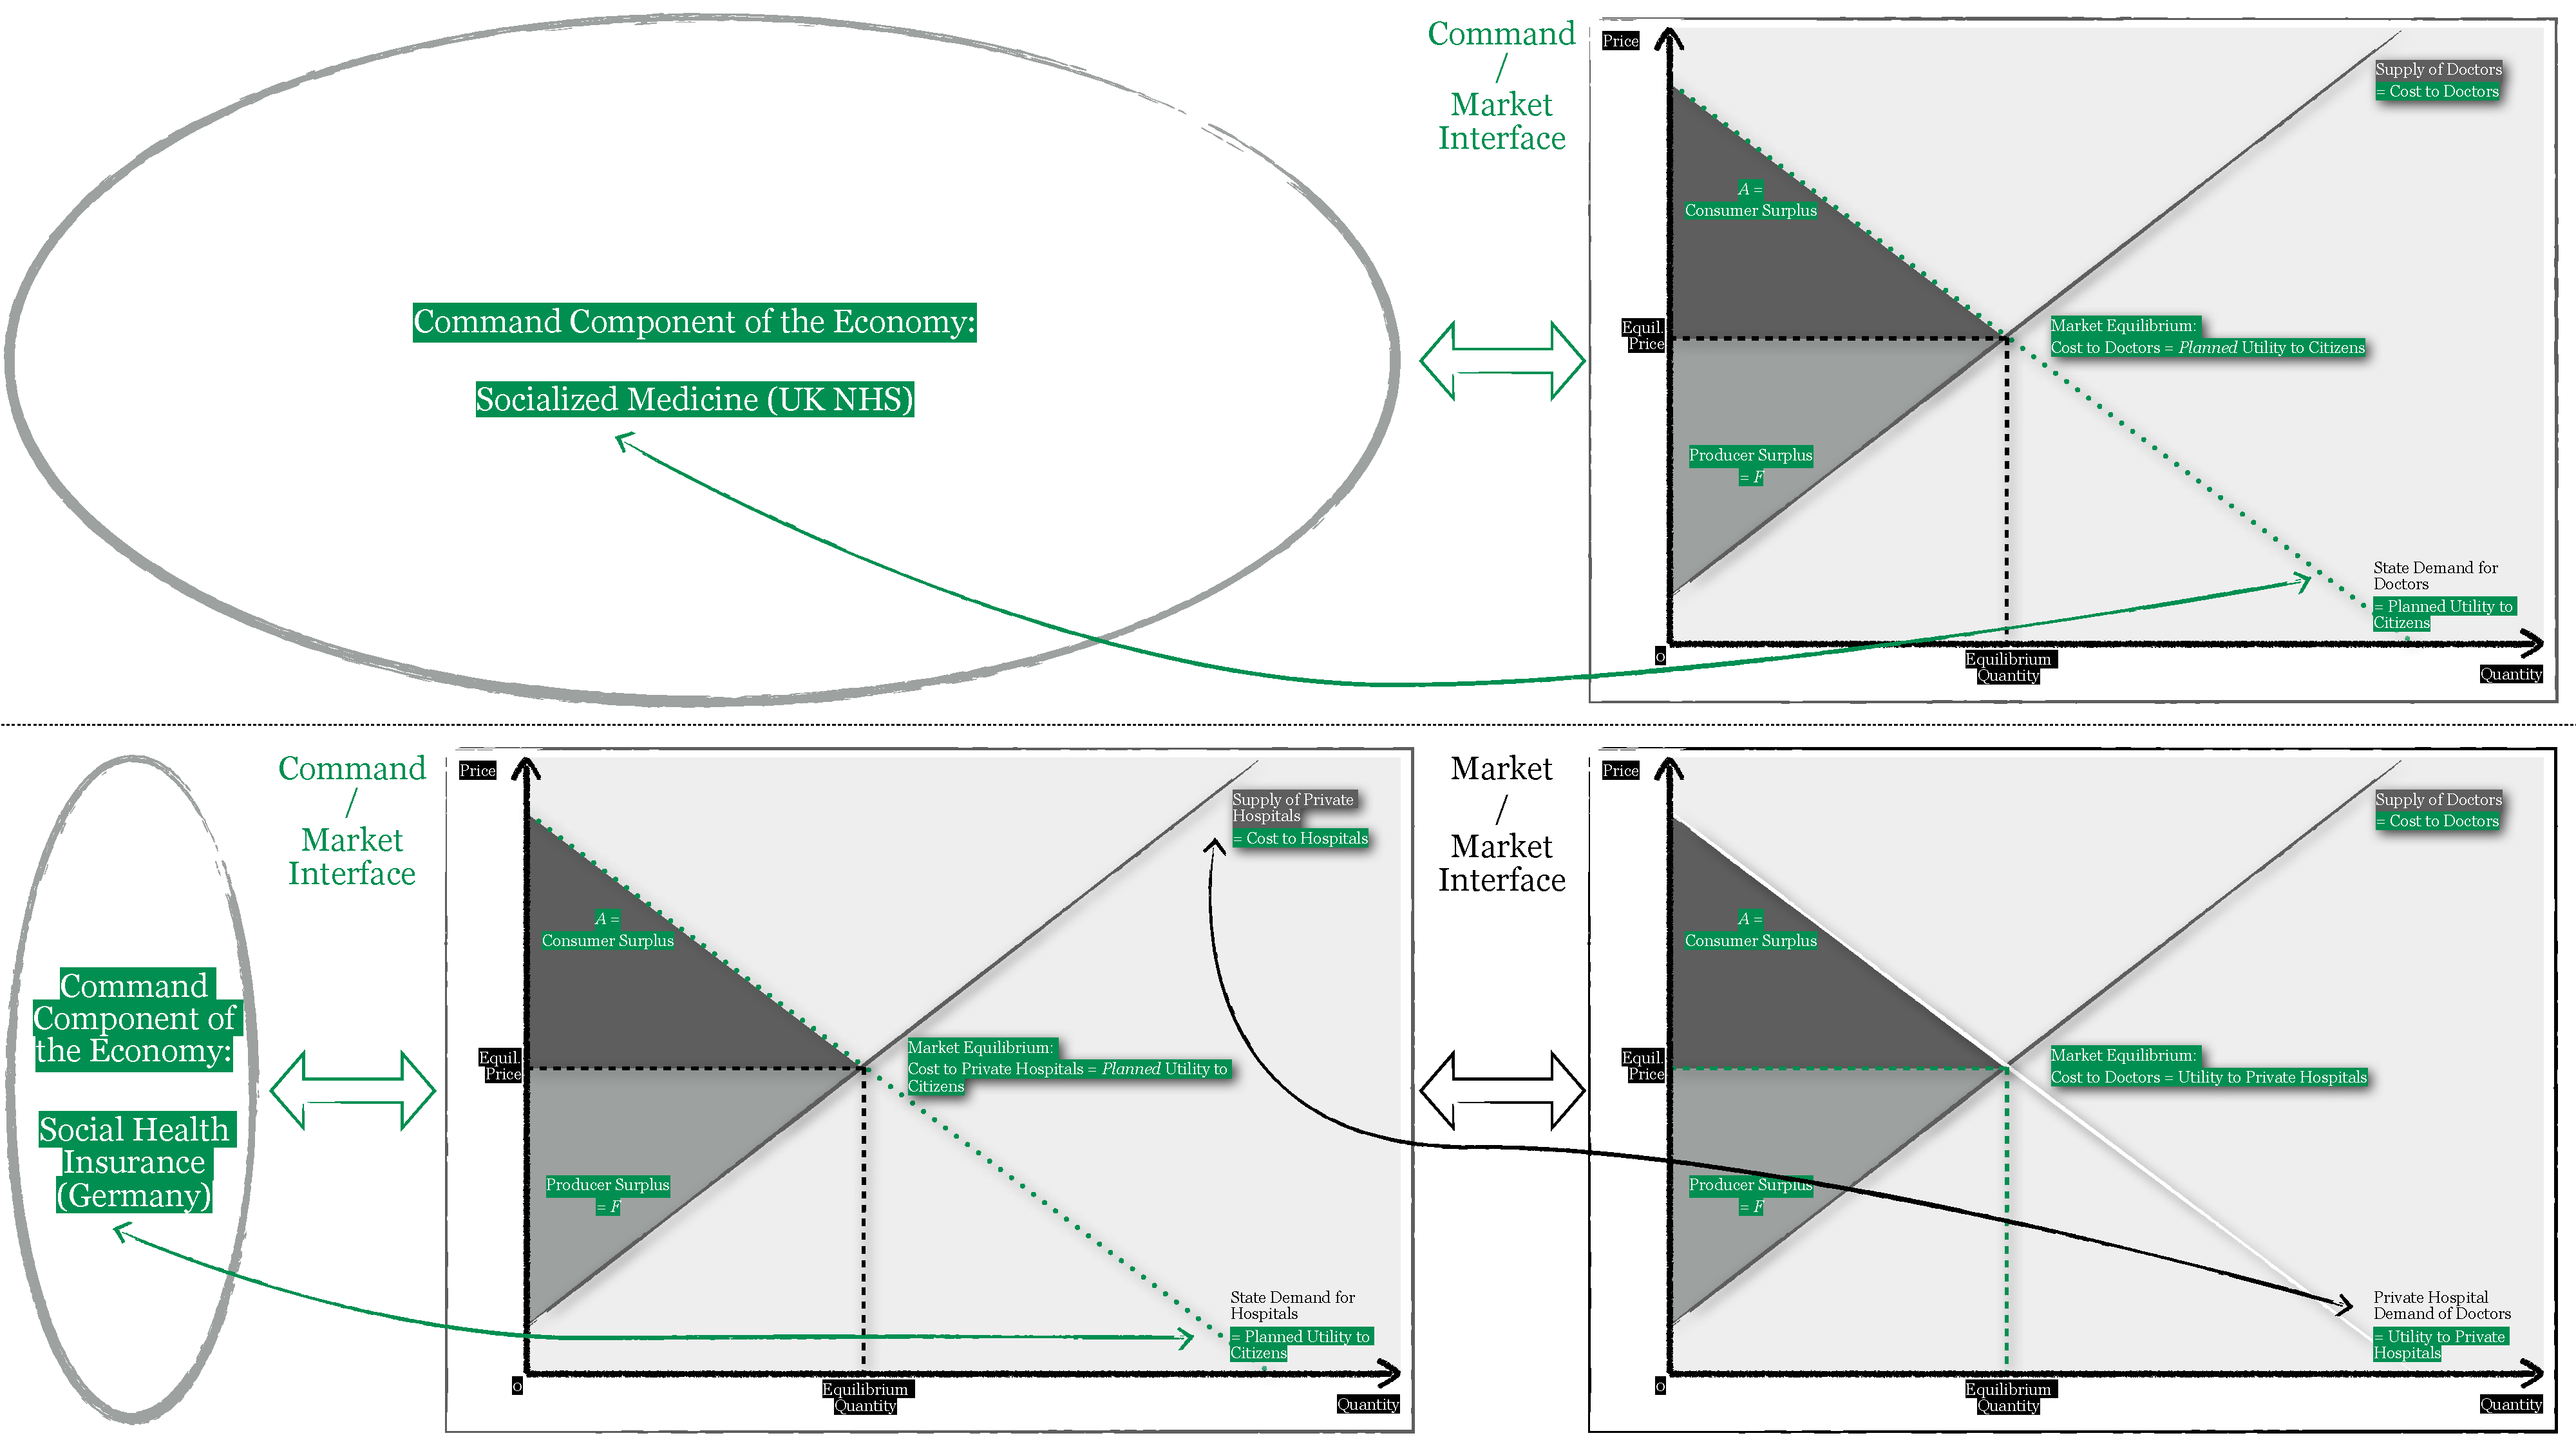
\includegraphics[width=1\textheight]{./img/interface-command-market-health}  
	\caption[Command-Market Interface in UK and German Healthcare]{The Command-Market Interface in UK and German Healthcare}
	\label{fig:interface-command-market-health}
	\end{center}
	\scriptsize{Market supply and demand are drawn in a conventional price-quantity diagram. For a larger version, see figure \ref{fig:supplydemand}. I discuss the \hyperref[sec:market-solutions-production]{competitive market equilibrium} later (p. \pageref{sec:market-solutions-production}).}
\end{figure}
\end{landscape}

\paragraph{Socialist Welfare State is an Oxymoron.} \gls{CEEC} member states of the European Union (EU-27) up to around 1990 were \emph{planned} (if not quite command) economies. As such, no matter their (however corrupted) socialist distributional goals, they \emph{were no} welfare states. Since the state directed much of both production and distribution, it did not need the (welfare state) institutions governing the mixed economy, such as including taxation, insurance and pension funds, business cycle smoothing and dedicated social service provision. Even where these institutions nominally existed, they never faced the (otherwise defining) condition of independent market prices. For example, where ``prices'' are \emph{set} and ``profits'' owned by the state, taxes become a meaningless category: they are really just changes in the set prices (e.g., \citealt{Bonker2006}: 23).

Consequently, \glspl{CEEC} built new welfare states institutions from scratch when they liberalized their markets during the 1990s and joined the EU in the 2000s. %kill this sentence for diss

\subsection[Ends]{The Ends of a Mixed Economy\footnote{
	Parts of this section are based on Chapter 2 of my Thesis for the Master of Public Policy at the Hertie School of Governance \citep{Held2010a}. I have greatly reworked, organized and added to the original version.}} \label{sec:ends}
If the defining characteristic of a welfare state is its uneasy union of market and plan, we must first understand the broader interplay of exchange and command in the mixed economy. Table \ref{tab:endsmixedeconomy} summarizes exchange (or market) and command (or state) institutions to address five material dimensions of the human condition: \hyperref[sec:production]{production}, \hyperref[sec:risk]{risk}, \hyperref[sec:distribution]{distribution}, \hyperref[sec:time]{time} and \hyperref[sec:space]{space}. This is a slightly expanded set, inspired by \citeauthor{MusgThet1959}'s \citeyearpar{MusgThet1959} seminal definition of basic public policy functions: allocation/efficiency, distribution and stabilization (e.g. as cited in \citealt{Bordo2011}: 4).

%include somewhere samuelsons' mixed economy, the giant of post ww economics: 1) redistribute 2) do public goods 3) stabilize the macro economy.

%cite stiglitz on the mixed economy synthesis (the price of ...)

	%!TEX root=../tax-democracy-held.tex

\begin{landscape}
 \begin{table}[htbp]
	\begin{center}
	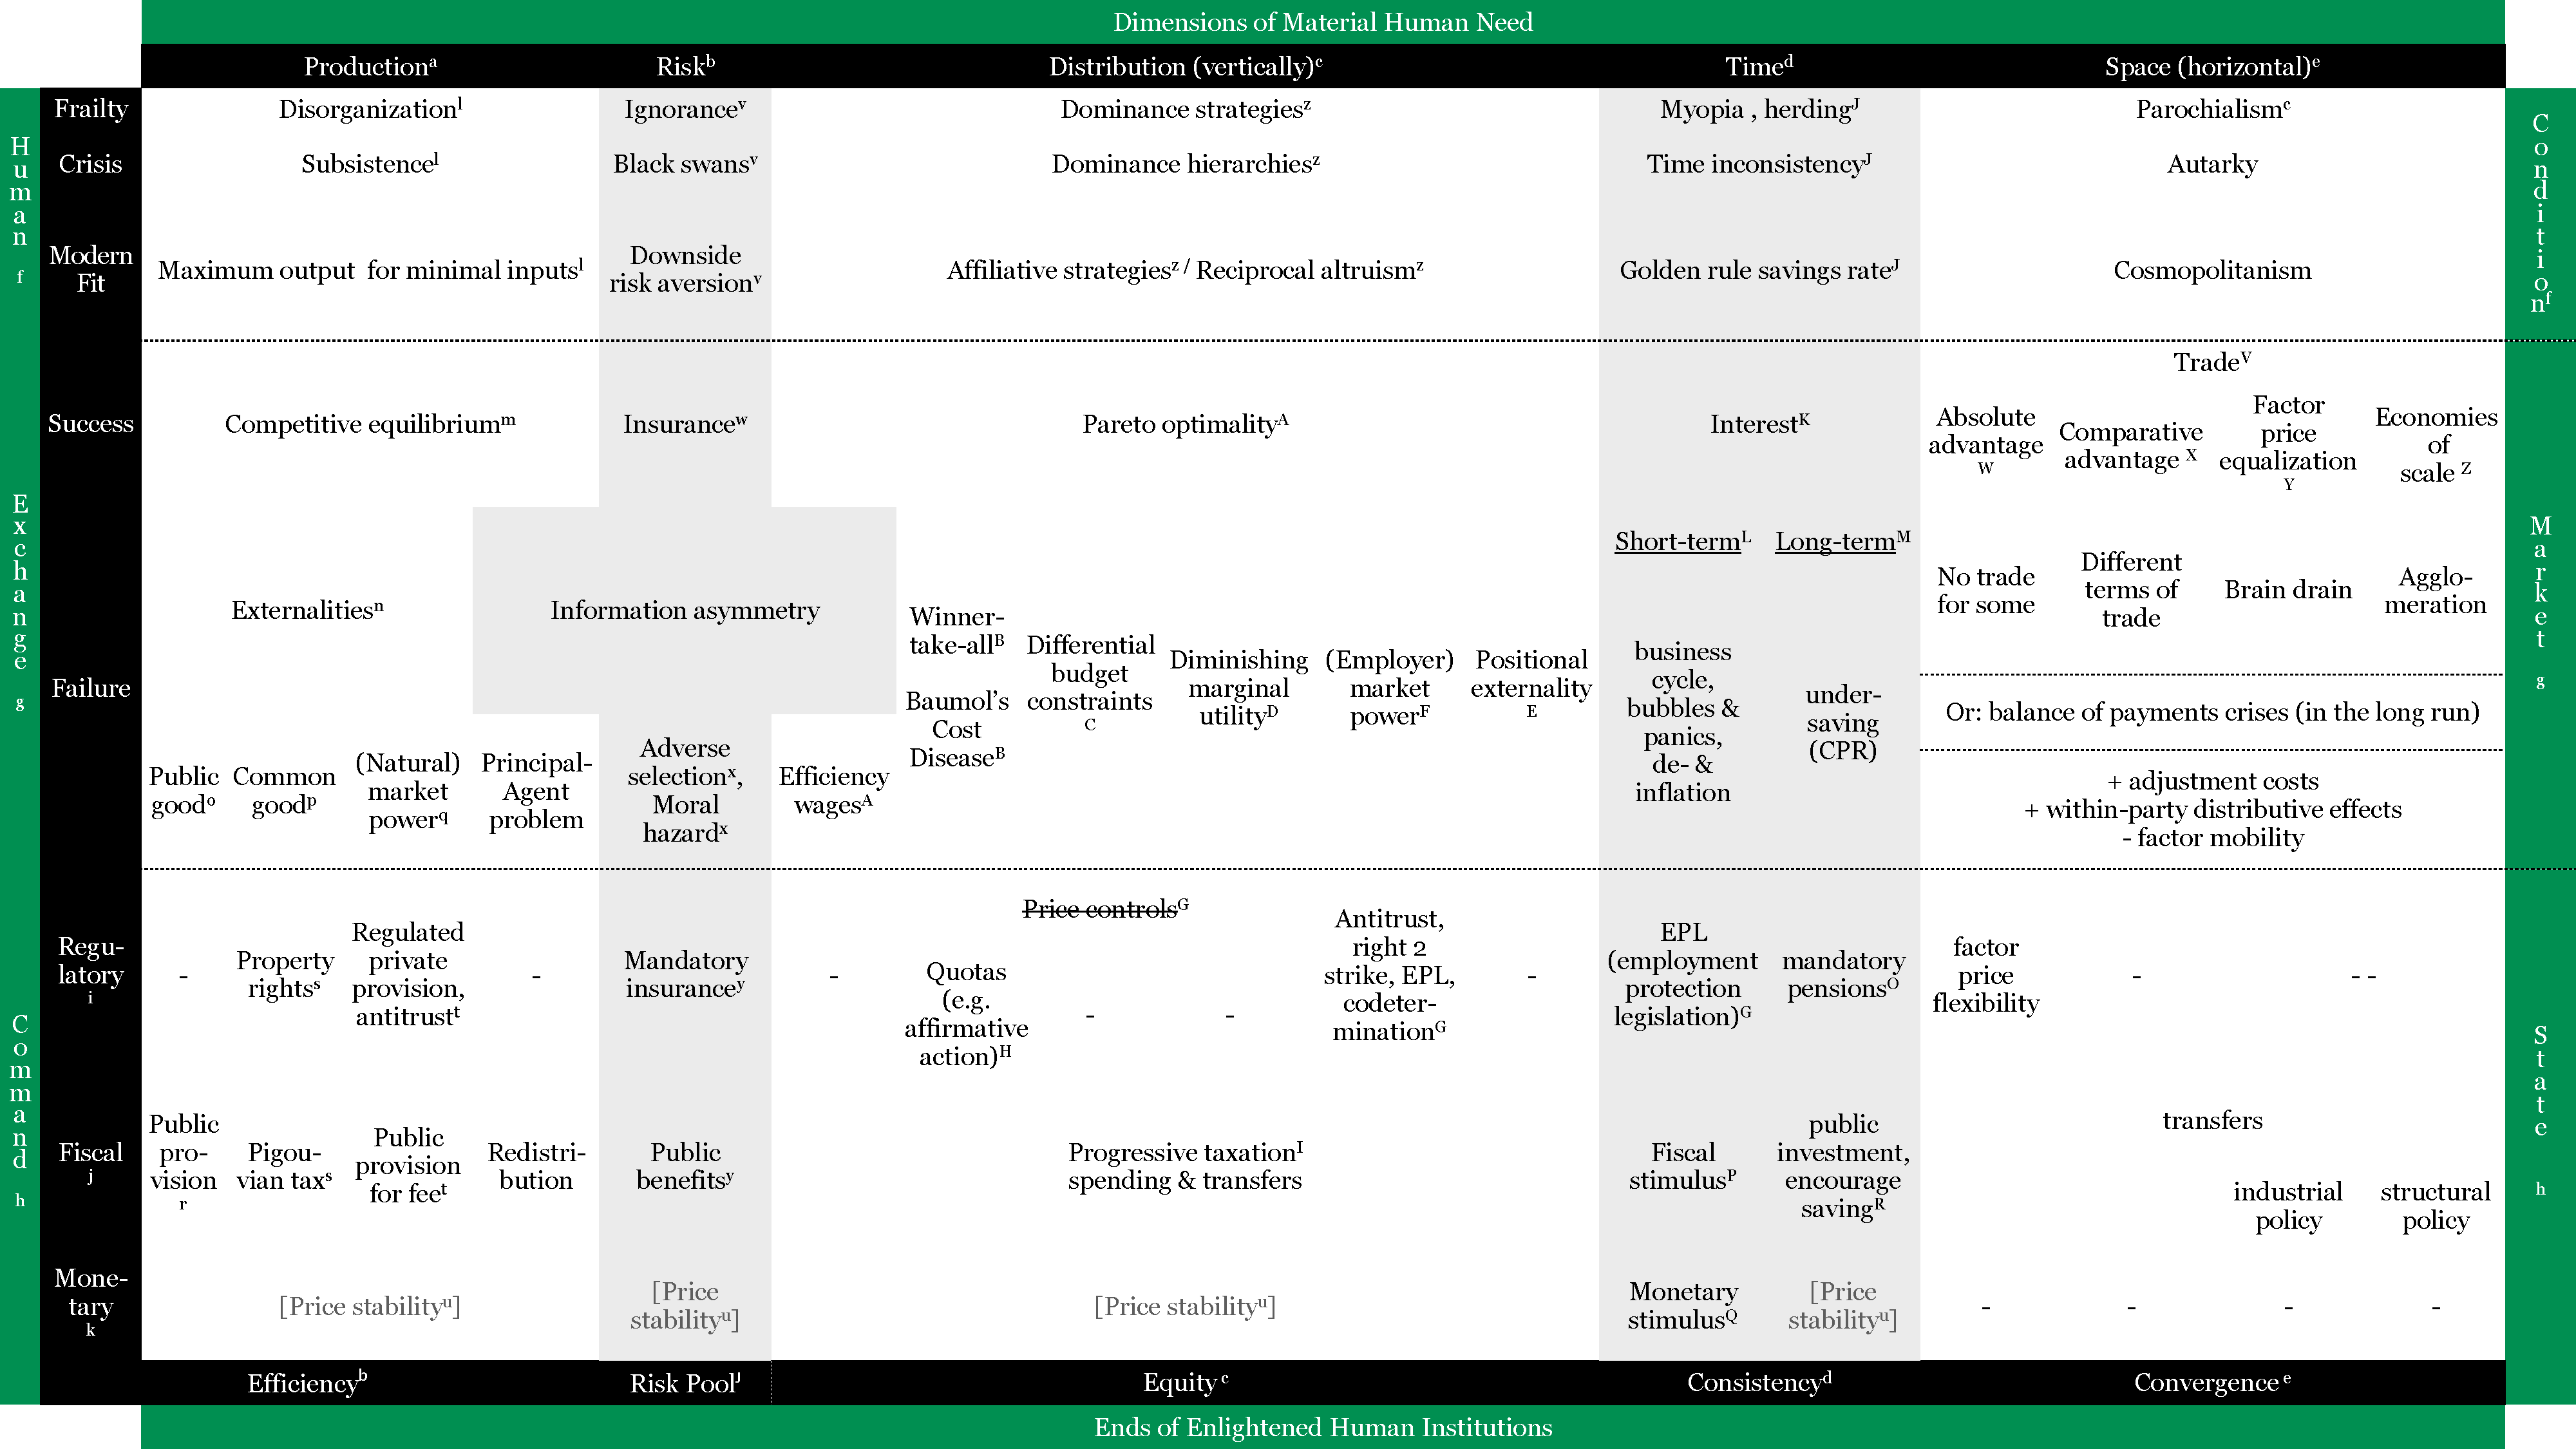
\includegraphics[width=1\linewidth]{ends-mixed-economy}
	\caption{Ends of the Mixed Economy \label{tab:ends-mixed-economy}}
\end{center}
\newpage
\end{table}
\end{landscape}\footnote{
Read the table from top to bottom, then from left to right. For every material dimension (column), I first present the human condition (first three rows), then market (exchange) solutions and problems (next two rows) and then present corresponding state (command) responses by fiscal, regulatory and monetary means (bottom three rows). The headings of following sections correspond to the column headings.

		\emph{a}: \nameref{sec:production} on page \pageref{sec:production},
		\emph{b}: \nameref{sec:risk} on page \pageref{sec:risk},
		\emph{c}: \nameref{sec:distribution} on page \pageref{sec:distribution},
		\emph{d}: \nameref{sec:time} on page \pageref{sec:time},
		\emph{e}: \nameref{sec:space} on page \pageref{sec:space},
		\emph{f}: \nameref{sec:human-condition} on page \pageref{sec:human-condition},
		\emph{g}: \nameref{sec:exchange} on page \pageref{sec:exchange},
		\emph{h}: \nameref{sec:command} on page \pageref{sec:command},
		\emph{i}: \nameref{sec:regulatory} on page \pageref{sec:regulatory},
		\emph{j}: \nameref{sec:fiscal} on page \pageref{sec:fiscal},
		\emph{k}: \nameref{sec:monetary} on page \pageref{sec:monetary},
		\emph{l}: \nameref{sec:human-nature-of-production} on page \pageref{sec:human-nature-of-production},
		\emph{m}: \nameref{sec:market-solutions-production} on page \pageref{sec:market-solutions-production},
		\emph{n}: \nameref{sec:market-failures} on page \pageref{sec:market-failures} and see \autoref{tab:types-of-goods},
		\emph{o}: \nameref{sec:public-good} on page \pageref{sec:public-good},
		\emph{p}: \nameref{sec:common-good} on page \pageref{sec:common-good},
		\emph{q}: \nameref{sec:natural-monopoly} on page \pageref{sec:natural-monopoly},
		\emph{r}: \nameref{sec:public-good-response} on page \pageref{sec:public-good-response},
		\emph{s}: \nameref{sec:common-good-response} on page \pageref{sec:common-good-response},
		\emph{t}: \nameref{sec:natural-monopoly-response} on page \pageref{sec:natural-monopoly-response},
		\emph{u}: \nameref{sec:price-stability} on page \pageref{sec:price-stability},
		\emph{v}: \nameref{sec:human-nature-of-risk} on page \pageref{sec:human-nature-of-risk},
		\emph{w}: \nameref{sec:insurance} on page \pageref{sec:insurance},
		\emph{x}: \nameref{sec:asymmetric-information} on page \pageref{sec:asymmetric-information},
		\emph{y}: \nameref{sec:state-insurance} on page \pageref{sec:state-insurance},
		\emph{z}: \nameref{sec:human-nature-of-inequality} on page \pageref{sec:human-nature-of-inequality},
		\emph{A}: \nameref{sec:market-equity} on page \pageref{sec:market-equity},
		\emph{AA}: \nameref{sec:efficiency-wages} on page \pageref{sec:efficiency-wages},
		\emph{B}: \nameref{sec:winner-take-all} on page \pageref{sec:winner-take-all},
		\emph{C}: \nameref{sec:different-budget-constraints} on page \pageref{sec:different-budget-constraints},
		\emph{D}: \nameref{sec:diminishing-marginal-utility} on page \pageref{sec:diminishing-marginal-utility},
		\emph{F}: \nameref{sec:monopsony-employers} on page \pageref{sec:monopsony-employers},
		\emph{E}: \nameref{sec:positional-race} on page \pageref{sec:positional-race},
		\emph{G}: \nameref{sec:price-controls} on page \pageref{sec:price-controls},
		\emph{H}: \nameref{sec:affirmative-action} on page \pageref{sec:affirmative-action},
		\emph{I}: \nameref{sec:fiscal-redistribution} on page \pageref{sec:fiscal-redistribution},
		\emph{J}: \nameref{sec:time} on page \pageref{sec:time},
		\emph{K}: \nameref{sec:interest} on page \pageref{sec:interest},
		\emph{L}: \nameref{sec:short-term-inconsistency} on page \pageref{sec:short-term-inconsistency},
		\emph{M}: \nameref{sec:long-term-inconsistency} on page \pageref{sec:long-term-inconsistency},
		\emph{O}: \nameref{sec:government-saves} on page \pageref{sec:government-saves},
		\emph{P}: \nameref{sec:fiscal-stimulus} on page \pageref{sec:fiscal-stimulus},
		\emph{Q}: \nameref{sec:monetary-stimulus} on page \pageref{sec:monetary-stimulus},
		\emph{R}: \nameref{sec:government-saves} on page \pageref{sec:government-saves},
		\emph{S}: \nameref{sec:government-saves} on page \pageref{sec:government-saves},
		\emph{V}: \nameref{sec:trade} on page \pageref{sec:trade},
		\emph{W}: \nameref{itm:absolute-advantage} on page \pageref{itm:absolute-advantage},
		\emph{X}: \nameref{itm:comparative-advantage} on page \pageref{itm:comparative-advantage},
		\emph{Y}: \nameref{itm:FPE} on page \pageref{itm:FPE},
		\emph{Z}: \nameref{itm:NTT} on page \pageref{itm:NTT}.}

% \begin{table}[htbp]
	%	\centering
	%	\rotatebox{90}{
	%	\begin{minipage}{\textheight}
	%	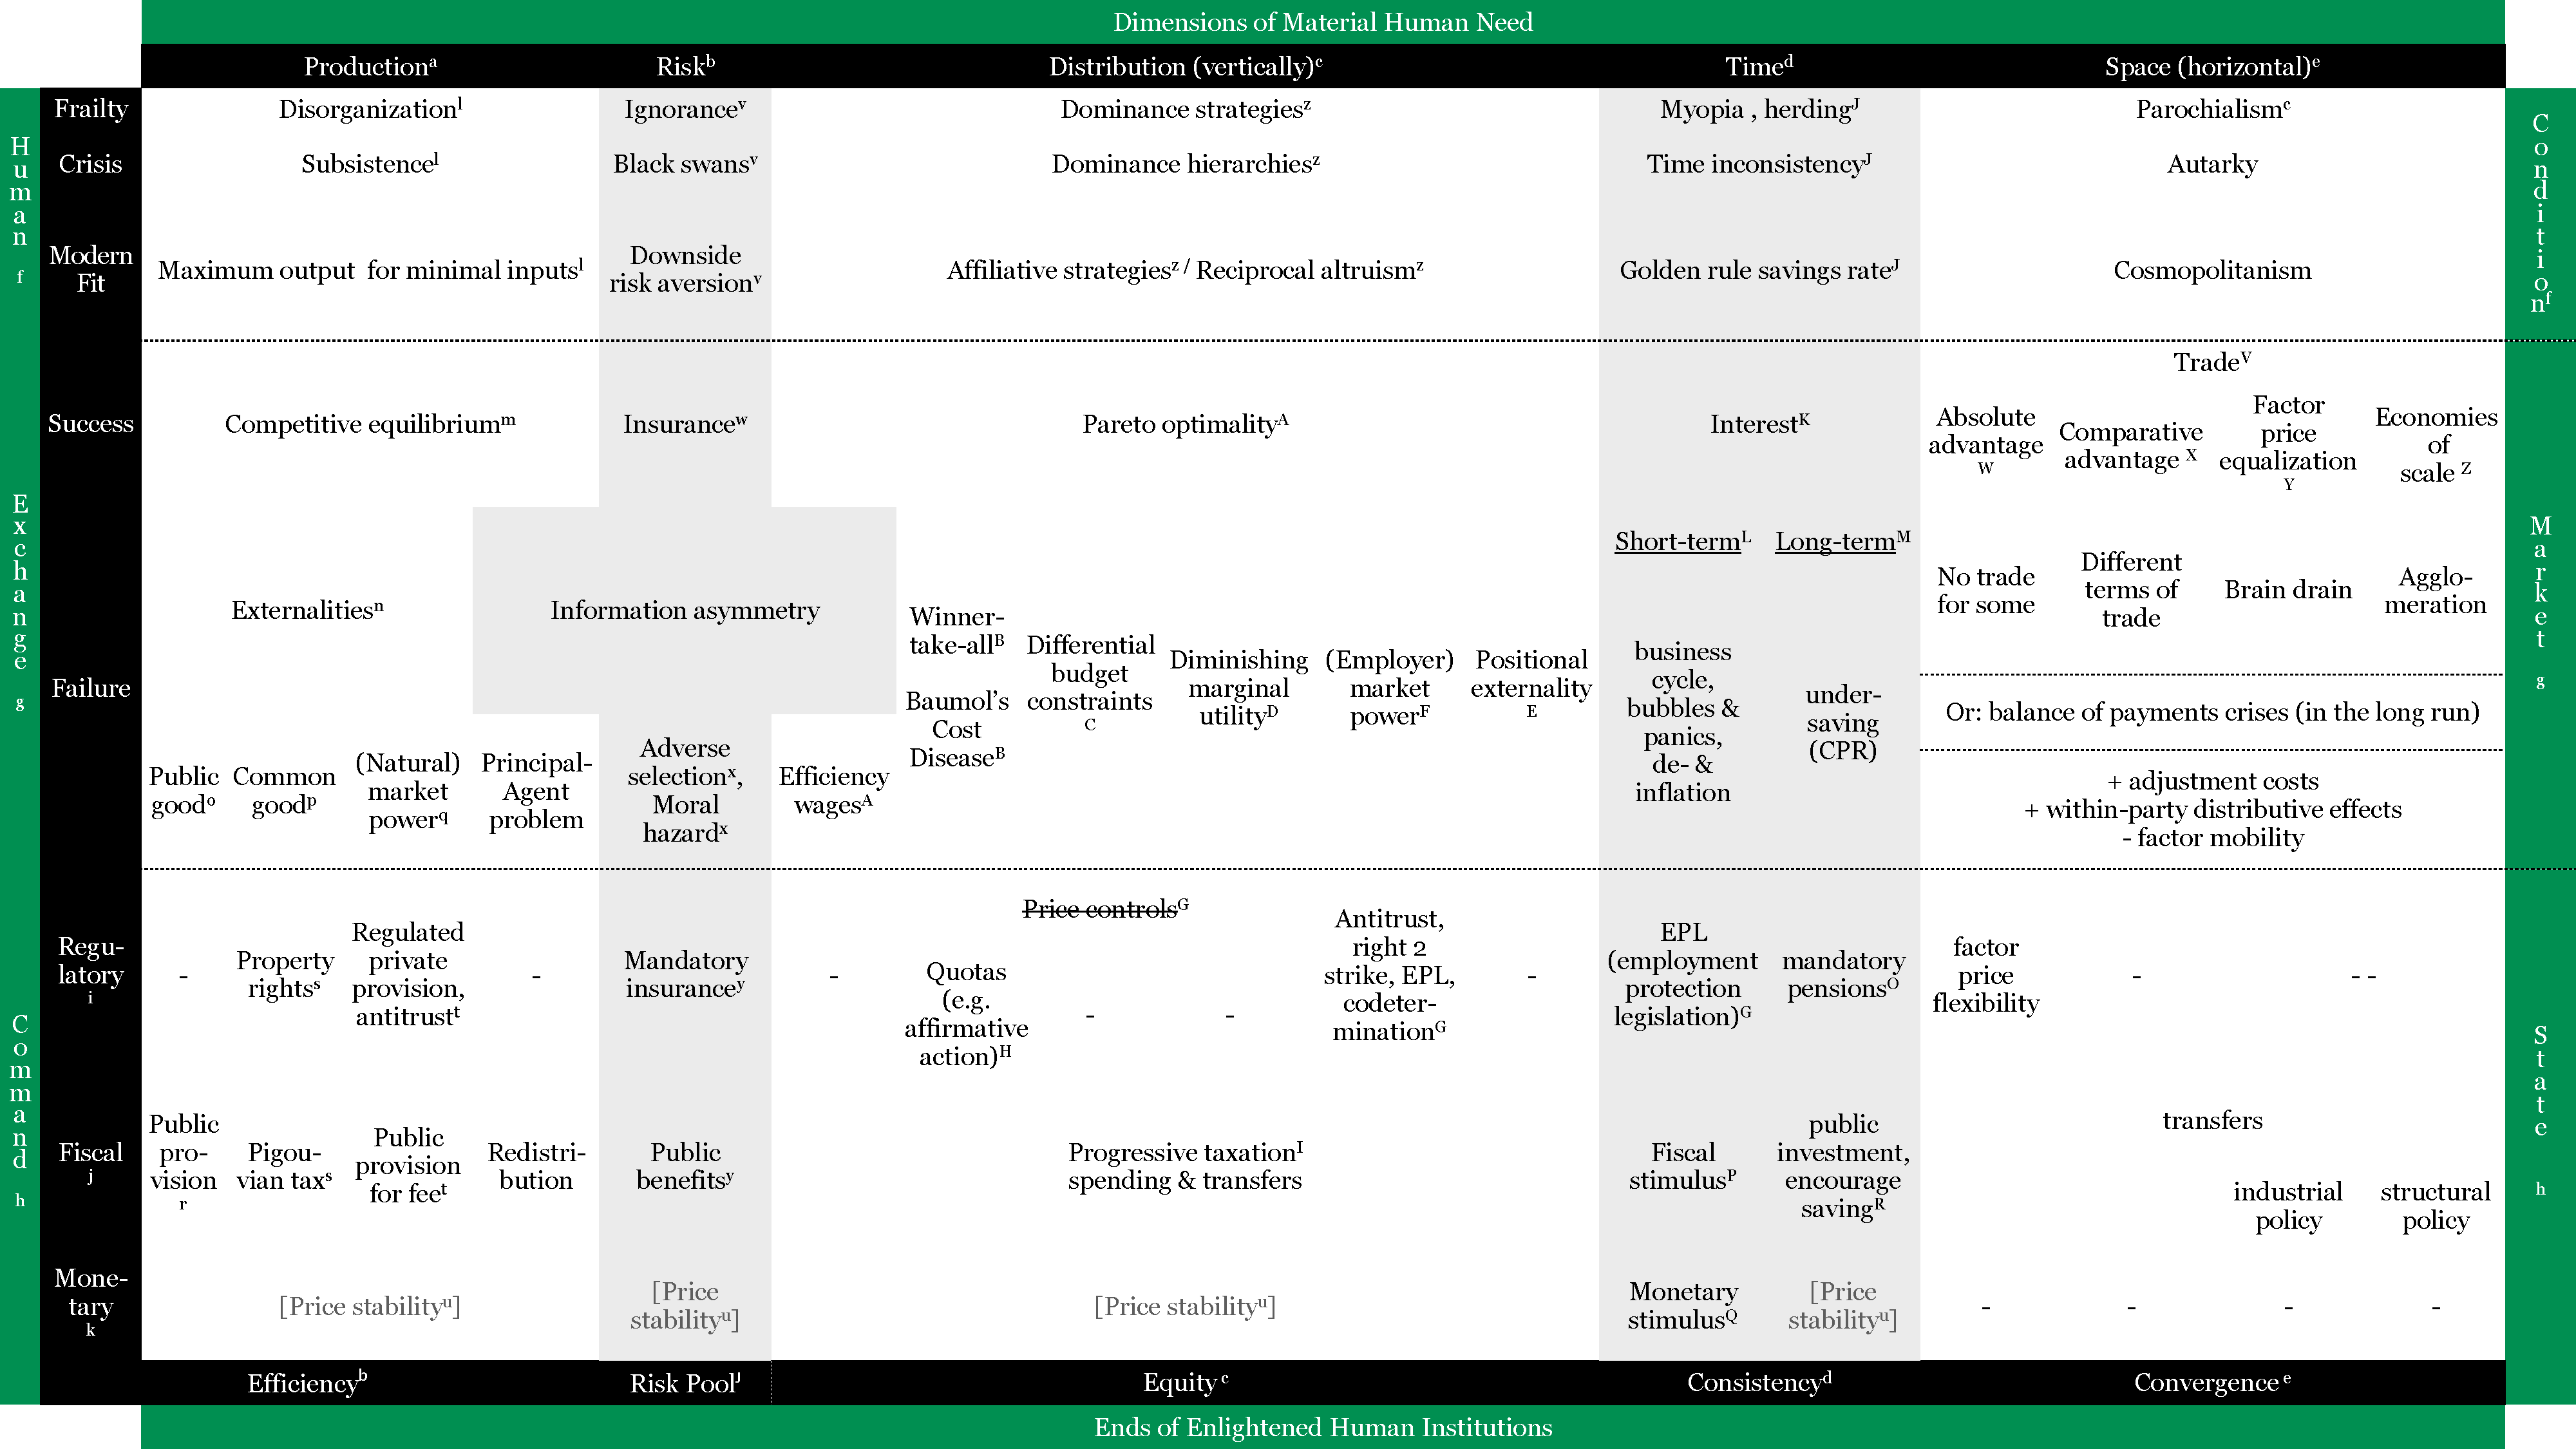
\includegraphics[width=1\linewidth]{ends-mixed-economy}
	%	\caption{Ends of the Mixed Economy}
	%	\label{tab:ends-mixed-economy}
	%	\end{minipage}
	%	}
%\end{table}

%\includepdf[landscape=true , fitpaper=true, frame=true ]{ends-mixed-econ}
	%if you want to go back and use this, you have to enable pdfpages package

\paragraph{The Human Condition.} \label{sec:humancondition}  Humans are a frail and feeble species and depend on a favorable physical and social environment (fit) to thrive. Exactly what the frailties of the human condition\footnote{
	\label{fn:humancondition}I choose the term ``human condition'', because it captures what is inescapable in human existence without relying on one or another natural or cultural explanation. Sociobiologists like \cite{Boyd1985} and recently \cite{Henrich2007} have argued for a co-evolution of genes and memes, rendering the nurture-vs-nature debate moot.}
are, and how we can live is of course controversial. I ground the mixed economy in human needs (rows 1--3 in table \ref{tab:endsmixedeconomy}) to provide context\footnote{
	Some of the frailties follow the heuristics and biases of human cognition identified by the prospect theory research program (\citealt{Kahneman1979}, recently \citealt{Kahneman2011}). Prospect theory is appropriate to consider for any first-order theory on the material: it provides a positively descriptive model of human decision making as opposed to the normatively optimal (but rarely observed) expected utility hypothesis, on which neoclassical economics rest (first formulated by \citealt{Bernoulli1738}, later specified by \citealt{VonNeumann1944}). In part, the mixed economy and the welfare state (e.g. mandatory pensions) are institutions to get prospect theory humans to make decisions based on expected utility. Prospect theory, alas, is still an emerging field (together with yet dejunct evolutionary psychology and cognitive neuroscience), and any link to the mixed economy must in the meantime remain tenuous.} 
and to focus on the first-order ends (bottom row) that the institutions of the mixed economy are to serve on these five dimensions (columns): \emph{efficient} \hyperref[sec:production]{production}, \emph{precaution} against \hyperref[sec:risk]{risk}, an \emph{equitable} \hyperref[sec:distribution]{distribution}, \emph{consistency} over \hyperref[sec:time]{time} and \emph{convergence} over \hyperref[sec:space]{space}.

\paragraph[Exchange]{Exchange.} \phantomsection \label{sec:exchange} 
Markets organize production by institutionalized, voluntary exchange of private property rights. They orchestrate both the production and the distribution of goods in \emph{one} system (rows 4--6). Markets \hyperref[sec:marketsolutionsproduction]{succeed} when they efficiently allocate resources and, equivalently, effectively process dispersed information (p. \pageref{sec:marketsolutionsproduction}). Markets also \hyperref[sec:marketfailures]{fail}, cause excessive inequity and risky imbalances (p. \pageref{sec:marketfailures}). 

\paragraph[Command]{Command.} \phantomsection \label{sec:command} The mixed economy is the set of \hyperref[sec:regulatory]{regulatory} (p. \pageref{sec:regulatory}), \hyperref[sec:fiscal]{fiscal} (p. \pageref{sec:fiscal}) and \hyperref[sec:monetary]{monetary} (p. \pageref{sec:monetary}) policies to mitigate market failures and to alter undesirable distributive outcomes (rows 6--8).

\paragraph{State-Market Coevolution.} Table \ref{tab:endsmixedeconomy} does not imply a historical or conceptual primacy of the market over the state, or vice versa. Production and distribution by exchange did not necessarily predate production and distribution by command, they \emph{co-evolved} (\citealt{Tilly-1985-aa}, also see footnote \ref{fn:tilly}). Likewise, production and distribution by command is no more a stop-gap measure to failures of a market economy than market provision is a stop-gap to government waste\footnote
	{Indeed, as Dr. Mildner of the Hertie School of Governance never tired of telling me: ``There is state failure, too''. \\
	Table \ref{tab:endsmixedeconomy} or the whole piece could be reorganized to start out with command solutions and problems, to which market institutions then respond. For example, governments may be inapt at producing diverse and fashionable clothing (as suggested by the late \href{http://kimjongillookingatthings.tumblr.com/}{Kim-Jong Il's choice of grey jumpsuits}), which is then spun off to markets.}. 
Neither markets nor states are superior, they are just better modes of producing and distributing \emph{different} things.

As table \ref{tab:endsmixedeconomy} stands, the game appears stacked against the market, as there is no list of government failures. In fact, failures abound in the command economy: without credible information about individual utility (cf. \citealt{Hayek1931}), and an elegant mechanism for their aggregation (cf. \citealt{Lerner1944, Lange1934, Debreu1954}) resources are wasted and misallocated. Moreover, the market economy and liberal democracy seem to be closely related\footnote{
	As in modernization theory, e.g. \cite{InglehartWelzel-2005-aa}.} 
and bloated command economies may corrupt politics\footnote{
	Specifically, resource-based ``rentier states'' may hinder liberal democracy \citep{Beblawi1990}. Generally, distributive decisions in planned economies appear easily as zero-sum games (as opposed to the per-definition positive-sum, pareto improvements in competitive markets), which may corrupt politics.} 
or even threaten the very constitution of freedom \citep{Hayek1944, Friedman1962}.

Here again\footnote
	{To ``economize on moral disagreement'' (\citealt{GutmannThompson-2004-aa}: 7,  loc. 226) and to lend credence to my later conclusions.}
I conservatively place the burden of proof on the state: Production and distribution by markets should only be replaced or altered by command when the market can demonstrably not achieve the desired outcomes, that is, when problems materialize (row 4 in table \ref{tab:endsmixedeconomy}).

I now discuss the five material dimensions of human need in turn. 

\subsubsection[Efficient Production]{Efficient Production: Growing the Pie}\label{sec:production}

\paragraph{The Human Condition of Production}\phantomsection \label{sec:humanconditionofproduction}
Ever the ``hypercultural species'' (\citealt{Henrich2007}: loc 175), cooperative production, as much else, does not come to us robotically, or by instinct as it does to the eusocial insects \citep{Wilson2012}. Disposed by genes and memes to act selfishly\footnote
	{Following \emph{individual} selection.}, 
but also inclined to be generous\footnote
	{Altruistic behavior, according to \cite{Wilson2012} and before him \cite{Darwin1859}, is an emergent property of the \emph{group}, following group selection. According to mainstream sociobiology (and initially \citealt{Wilson1975}), altruism emerges at the \emph{individual} level by a strategy of inclusive fitness or genetic nepotism, helping others as they are related.} 
``we are stuck in-between'' \citep{Lehrer2012}. And so, again, we need institutions to regulate our cooperation. Without them, we are left in a debilitating state of \emph{disorganization} (column 1, row 1 in table \ref{tab:endsmixedeconomy})\footnote
	{In the modern world, this state can be observed in much of the developing world (cf. \citealt{Clark2007}, \citealt{Easterly-2006-aa}), war zones (e.g. \citealt{Baker-IIIHamilton-2006-aa} on Iraq) or wherever else human culture has regressed back to or stalled in innate (kin-, clan-) modes of cooperation (e.g. \citealt{PutnamLeonardi-1993-aa} on southern Italy).}.

The modern economy --- and indeed any known way to prosperity --- is knowledge intensive and based on the division of labor\footnote
	{These \hyperref[sec:sourcesofwealth]{sources of wealth} are discussed later (p. \pageref{sec:sourcesofwealth}).},
in other words, a highly cooperative enterprise. States and markets are, the atomistic rhetoric of \citeauthor{Hobbes-1651-aa} and \citeauthor{Smith-1776-lq} aside, a feat of great cooperation. Markets rely on private property rights and binding contracts, both of which are backed by the state, which in turn is a cooperative achievement\footnote{
	Expanding on \citeauthor{Tilly-1985-aa}'s account of state genesis, the cooperation problem of state-building lies between the different thugs making up the racketeering mafia, whose organization will eventually scale up to proto-state, then state. As Coppola's ``Godfather'' (1972, 1974, 1990) trilogy has shown, successful organized crime is not easy, and hinges on trust. Incidentally, in the case of the Corleone organization, cooperation is built on family ties, alluding to theories of inclusive fitness as nepotism.}.
Without market (or state) institutions to organize our production, we are left in a state of meager \emph{subsistence} (column 1, row 2 in table \ref{tab:endsmixedeconomy})\footnote
	{This state is aptly described by \cite{Malthus1798}: absent functional differentiation (or, equivalently, \emph{economies of scale}) mankind \emph{will}, by definition, be condemned to eternal poverty, as geometric population growth always outstrips \emph{arithmetric} economic growth. If somewhat amiss, historically --- functional differention was well under way in Malthus' time --- at a deep level, cooperation \emph{is} our ticket out of hardship, a notion to which I return in the \hyperref[sec:growthsolidarity]{conclusion} (p. \pageref{sec:growthsolidarity}).}

Humans, in a world of scarcity, must strive for institutions that deliver \emph{maximum outputs for minimal inputs}\footnote
	{This broad definition of efficiency is more demanding than pareto efficiency.} 
(see column 1, row 3 in table \ref{tab:endsmixedeconomy}).

\paragraph{Market Solutions to Production.} \phantomsection \label{sec:marketsolutionsproduction} Assuming, as I do, \hyperref[it:homoeconomicus]{homo economicus} (p. \pageref{it:homoeconomicus})  and conditions for \hyperref[sec:perfectcompetition]{perfect competition} (p. \pageref{sec:perfectcompetition}) markets have at least two attractive properties\footnote
	{Attractive in terms of conceptual clarity, not positive claim (perfect competition is rare) or normative appeal (ex-ante distributions are not a blank, egalitarian slate).}:
\begin{enumerate}
	\item when all  participants have made all profitable exchanges\footnote
		{(Neo)classical economics takes an oddly static view of the economy. In reality, equilibria are more often in flux, a matter of becoming, not being.}, 
	markets produce at the quantity and price where the costs to the producers equal the cost to buyers (see figure \ref{fig:supplydemand}). Consumers and producers in any given market enjoy maximum \emph{surplusses}: all consumers pay prices (at least incrementally) below the utility they receive (by area $A$), all producers receive prices (at least incrementally) above the costs they incur (by area $F$). In this \emph{competitive equilibrium} (see column 1, row 4 in table \ref{tab:endsmixedeconomy}), no one can be made better off without making someone else worse off: it is \emph{Pareto optimal}\footnote{
		\label{fn:1sttheorem} Formally, the first theorem of welfare economics states that over a \emph{given} distribution, the competitive equilibrium will be a pareto optimum (demonstrated first graphically by \cite{Lerner1944}, mathematically by \cite{Lange1934}, \cite{Debreu1954} and others).},
		\footnote{An allocation is pareto-improved if at least someone receives more, with others receiving (at least) the same. When all such improvements are exhausted, an allocation is pareto optimal. Crucially, pareto improvements and optimality are always in reference \emph{only} to some ex-ante allocation. Also, pareto improvements does not imply that everyone would be better off by the same amount.}. 
	\begin{figure}[htbp]
		\centering
		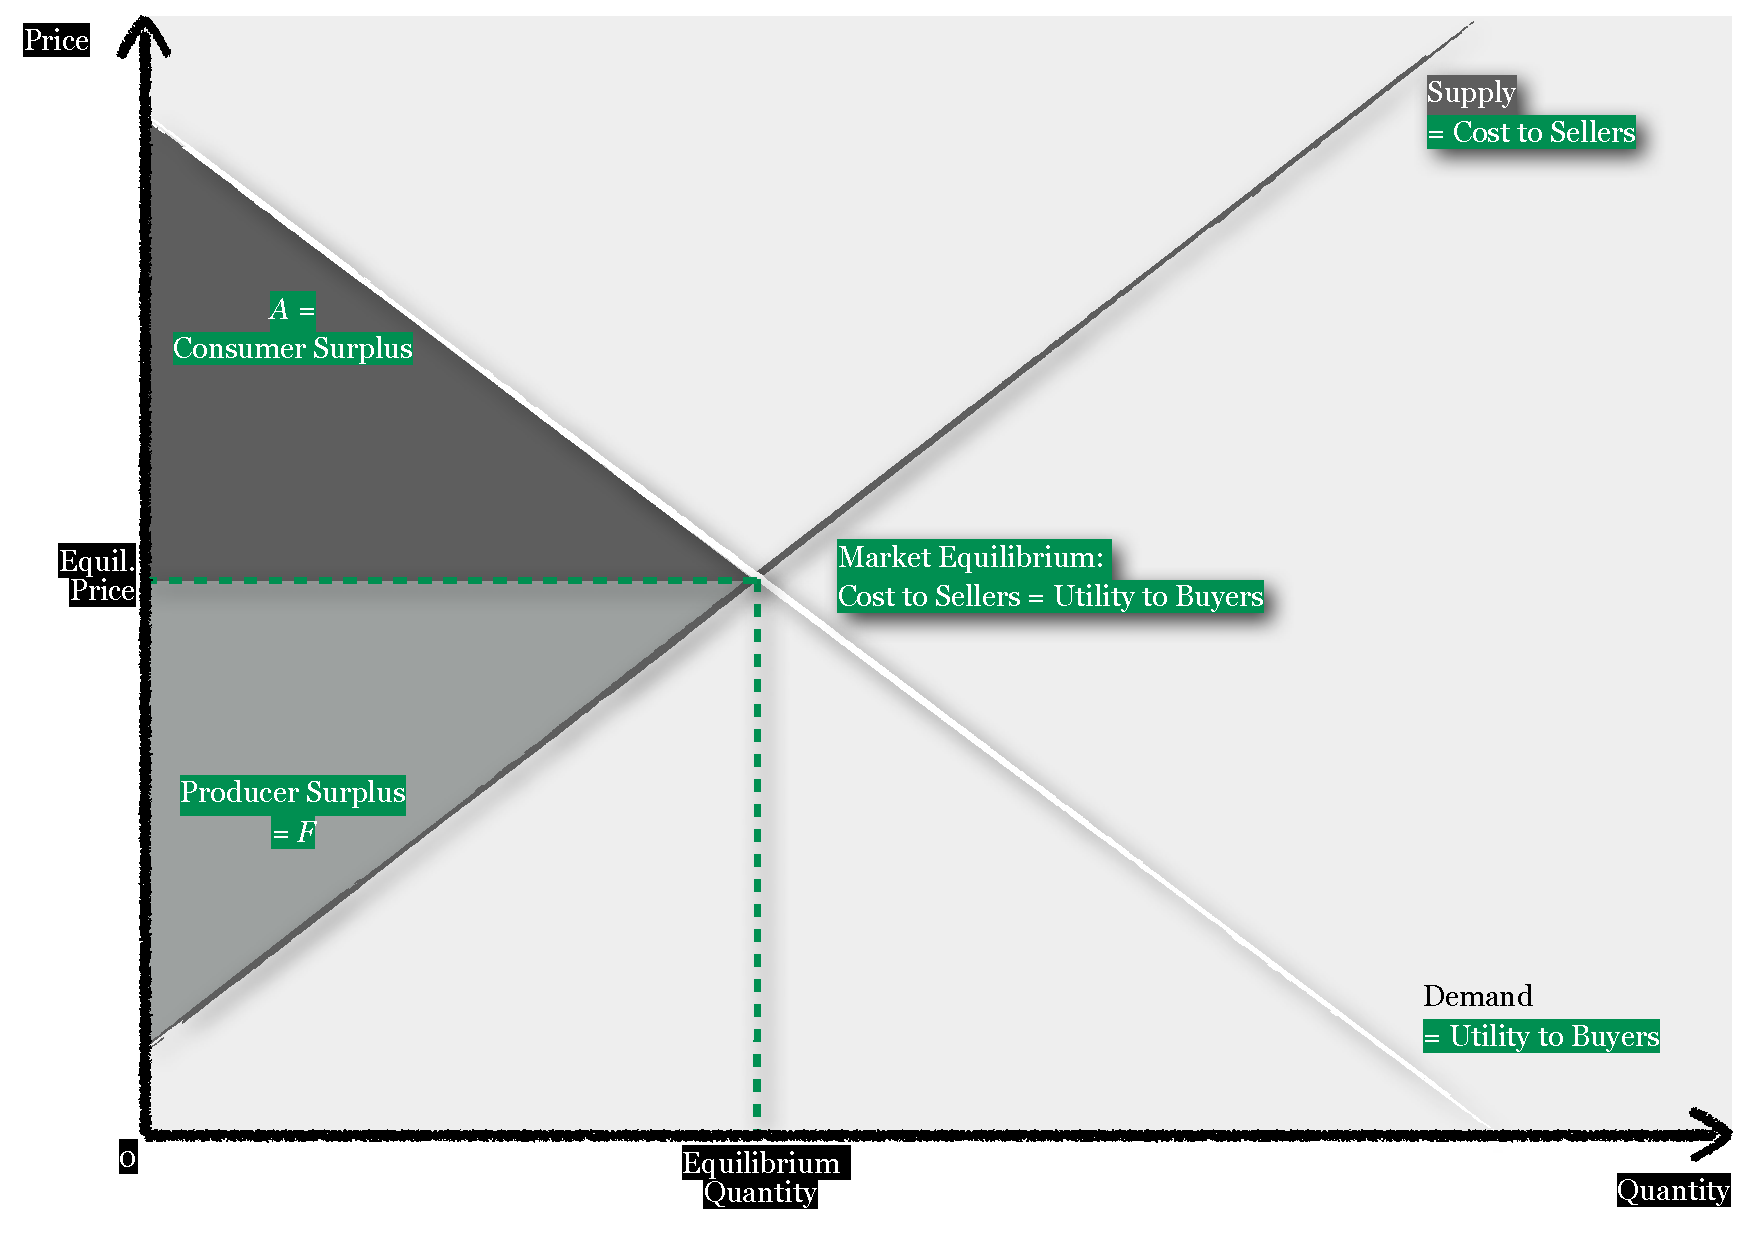
\includegraphics[width=1\textwidth]{./img/supply-demand}  
		\caption{Market Equilibrium of Supply and Demand}
		\label{fig:supply-demand}
	\end{figure}
	\item The \emph{price system} (see column 1, row 4 in table \ref{tab:endsmixedeconomy}) makes markets into supreme ``information processors'' \citep{Hayek1931}\footnote{
		Nassim Nicholas \cite{Taleb2007} has recently put this succinctly by praising ``aggressive trial and error'' (\emph{ibid.}: xxi) in free markets that ``allow people to be lucky'' (\emph{ibid.}: xxi). Being a quantitative trader by profession, \cite{Taleb2007} abandons rational choice when faulting Karl \cite{Marx-1867-aa} \emph{and} Adam \cite{Smith-1776-lq} for believing that free markets work because of rewards.}. 
	Because decisions are decentralized, markets can elegantly aggregate dispersed information where a central planner would have to gather them by bureaucratic means (such as a \gls{CBA}). Because market decisions are always backed by private costs, the market price system can reveal and communicate (some!) private information, where a central planner may face distorted (inflated) information about cost and utility.
\end{enumerate}

\subparagraph[Perfect Competition]{Conditions for Perfect Competition.} \label{sec:perfectcompetition} The above properties of market equilibria hold only under the strict assumptions of perfect or atomistic competition. In one formulation, this entails (\citealt{McDowell2006}: 157f.): 
\begin{enumerate}
	\item \emph{Infinite buyers and sellers}.\label{it:infinitebuyerssellers} There are so many consumers and producers in the market that any offer or bid by any one of them will have a negligible impact on prices. Everyone is a price taker.
	\item \emph{Zero barriers to entry and exit}. \label{it:easyentryexit} 
		Firms can start or cease to produce a good at relatively little cost and effort. All markets are wide open. 
	\item \emph{Perfect factor mobility.} \label{it:perfectfactormobility} 
		In the long run, labor, capital and other inputs to production can move to wherever they earn the highest rents. It is hire and fire.
	\item \emph{Perfect information}. \label{it:perfectinformation} 
		Consumers know all prices and qualities of goods, producers know all prices and qualities of factor inputs. People are omniscient and powerful calculators of utility.
	\item \emph{Profit-maximizing firms}. \label{it:profit-maximizingfirms} 
		Firms sell at the price and quantity that maximizes their profit\footnote{
			\citeauthor{Friedman1970a}'s dictum applies: ``The Social Responsibility of Business is to Increase its Profits'' \citeyearpar{Friedman1970a}, both as commandment and promised salvation.}.
		Other, exogenous criteria are not part of firm decision making. Given the other assumptions of perfect competition, firms sell where marginal cost equals marginal revenue.
	\item \emph{Homogeneous products.}\label{it:homogeneousproducts}
		Goods produced by one supplier are the same as those produced by another supplier of the same category. Inputs provided by one factor owner are the same as those provided by another owner of the same factor. All goods and factor inputs are completely commodified. 
\end{enumerate} 
To this, one might add, according to \citeauthor{Wikipedia2012}:
\begin{enumerate} \setcounter{enumi}{6}
	\item \emph{Zero transaction costs.} \label{it:zerotransactioncosts}
		Buyers and sellers face no costs making and exchange. Search, information, bargaining, policing and enforcement costs are assumed away. There is no friction.
	\item \emph{Constant returns to scale.} \label{it:constantreturnstoscale} 
		For any additional unit produced, costs rise by the same amount, no matter how much units are produced. The cost function is linear, marginal costs are constant. There are no (dis)economies of scale or scope. 
	
		Constant returns to scale are related to, but distinct from assumption \ref{it:easyentryexit} on \hyperref[it:easyentryexit]{easy entry and exit}.
	\item \emph{Property rights} \label{it:propertyrights} are well established. 
\end{enumerate}

I note wherever I relax some of these strict (and rarely plausible) assumptions in the following sections (summarized in table \ref{tab:assumptions-failures}).

	%!TEX root=../tax-democracy-held.tex

\begin{landscape}
\begin{table}
	\caption[Perfect Competition, Homo Economicus and Corresponding Market Failures]{Relaxing Assumptions about Perfect Competition and Homo Economicus and Corresponding Market Failures}
	\label{tab:assumptions-failures}
	\scriptsize
	\begin{center}
	\begin{tabular}{m{0.36\textwidth}*{10}{m{0.058\textwidth}}*{3}{m{0.09\textwidth}}}
		\toprule
		 & \multicolumn{10}{c}{\hyperref[sec:perfect-competition]{Perfect Competition Assumption} (p.~\pageref{sec:perfect-competition})} & \multicolumn{3}{c}{Homo Economicus}\\
		& %0
		\ref{itm:infinite-buyers-sellers} & %1
		\ref{itm:easy-entry-exit} & %2
		\ref{itm:perfect-factor-mobility} & %3
		\ref{itm:perfect-information} & %4
		\ref{itm:profit-maximizing-firms} & %5
		\ref{itm:homogeneous-products} & %6
		\ref{itm:zero-transaction-costs} & %7
		\ref{itm:constant-returns-to-scale} & %8
		\ref{itm:property-rights} & %9
		\ref{itm:same-budgets} & %10
		Indi-vidually & %11
		Rational &  %12
		Utility-Maximizer  \\ %13

		& %0
		p.~\pageref{itm:infinite-buyers-sellers} & %1
		p.~\pageref{itm:easy-entry-exit} & %2
		p.~\pageref{itm:perfect-factor-mobility} & %3
		p.~\pageref{itm:perfect-information} & %4
		p.~\pageref{itm:profit-maximizing-firms} & %5
		p.~\pageref{itm:homogeneous-products} & %6
		p.~\pageref{itm:zero-transaction-costs} & %7
		p.~\pageref{itm:constant-returns-to-scale} & %8
		p.~\pageref{itm:property-rights} & %9
		p.~\pageref{itm:same-budgets} & %10
		? & %11
		?  & %12
		?  \\ %13

		\midrule
		\hyperref[sec:public-good]{Public good} (p.~\pageref{sec:public-good}) & & & & & & & &X &X & &? & & \\

		\hyperref[sec:common-good]{Common good} (p.~\pageref{sec:common-good}) & & & & & & &X & &X & &? & & \\

		\hyperref[sec:natural-monopoly]{(Natural) market power} (p.~\pageref{sec:natural-monopoly}) &X &X & & & &X & &X & & & & & \\

		\hyperref[sec:principal-agent-problem]{Principal-agent problem} (p.~\pageref{sec:principal-agent-problem}) & & & &X & &X &X & & & & & & \\

		\hyperref[sec:adverse-selection]{Adverse selection} (p.~\pageref{sec:asymmetric-information}) & & & &X & &X & & & & & & & \\

		\hyperref[sec:moral-hazard]{Moral hazard} (p.~\pageref{sec:asymmetric-information}) & & & &X & & & & & & & & & \\

		\hyperref[sec:efficiency-wages]{Efficiency wages} (p.~\pageref{sec:efficiency-wages}) & & & &X & &X &X & & & & & & \\

		\hyperref[sec:winner-take-all]{Winner-take-all} (p.~\pageref{sec:winner-take-all}) & &X & & & & & &X & & & & & \\

		\hyperref[sec:different-budget-constraints]{Different budget constraints} (p.~\pageref{sec:different-budget-constraints}) & & & & & & & & & &X & & &? \\

		\hyperref[sec:diminishing-marginal-utility]{Diminishing marginal utility} (p.~\pageref{sec:diminishing-marginal-utility}) & & & & & & & &X & &? & & &? \\

		\hyperref[sec:monopsony-employers]{(Employer) market power} (p.~\pageref{sec:monopsony-employers}) &X &X &X & & & & &X & & & & & \\

		\hyperref[sec:positional-race]{Positional externality} (p.~\pageref{sec:positional-race}) & & & & & & & & &X & &X & &X \\

		\hyperref[sec:short-term-inconsistency]{Business cycle} (p.~\pageref{sec:short-term-inconsistency})& & & & & & & & & & & &? & \\

		\hyperref[sec:short-term-inconsistency]{Bubbles \& panics} (p.~\pageref{sec:short-term-inconsistency}) & & & & & & & & & & &? &? & \\

		\hyperref[sec:short-term-inconsistency]{De-/Inflation} (p.~\pageref{sec:short-term-inconsistency}) & & & & & & & & & & & &X & \\

		\hyperref[sec:long-term-inconsistency]{Undersaving Commons} (p.~\pageref{sec:long-term-inconsistency}) & & & & & & & & &X & &? & \\

		\hyperref[itm:absolute-advantage]{No trade for some} (p.~\pageref{itm:absolute-advantage}) & & &X & & & & & & & & & & \\

		\hyperref[itm:comparative-advantage]{Different terms of trade} (p.~\pageref{itm:comparative-advantage}) & & &X & & & & & & & & & & \\

		\hyperref[itm:FPE]{Factor price equalization} (p.~\pageref{itm:FPE}) & & &! & & & & & & & & & & \\

		\hyperref[itm:NTT]{Agglomeration} (p.~\pageref{itm:NTT}) &? &? &? & & & & &X & & & & & \\

		\midrule
			& %0
			\tiny \hyperref[itm:infinite-buyers-sellers]{Infinite buyers \& sellers} & %1
			\tiny \hyperref[itm:easy-entry-exit]{Easy entry \& exit} & %2
 			\tiny \hyperref[itm:perfect-factor-mobility]{Perfect factor mobility} & %3
			\tiny \hyperref[itm:perfect-information]{Perfect information} & %4
			\tiny \hyperref[itm:profit-maximizing-firms]{Profit maximization} & %5
			\tiny \hyperref[itm:homogeneous-products]{Homo-geneous products} & %6
			\tiny \hyperref[itm:zero-transaction-costs]{Zero transaction costs} & %7
			\tiny \hyperref[itm:constant-returns-to-scale]{Const. return to scale} & %8
			\tiny \hyperref[itm:property-rights]{Property rights} & %9
			\tiny \hyperref[itm:same-budgets]{Same budget constraints} &%10
			\tiny Indi-vidually & %11
			\tiny Rational &  %12
			\tiny Utility-Maximizer  \\ %13
		\bottomrule
	\end{tabular}
	\end{center}
\end{table}
\end{landscape}


\paragraph{Market Failures} \phantomsection \label{sec:market-failures} Markets operate efficiently on private goods: people can be \emph{excluded} from their \emph{rival} use (see table \ref{tab:types-of-goods}). In this case, social costs and utility match private cost and utility. 

From some goods, people cannot be effectively excluded and/or are not rivals in their consumption\footnote{
	I discuss only a popular subset of market failures in this paper. I ignore many of the problems recently highlighted by the 2007ff financial and sovereign debt crises. While common and public good failures explain much (for example herding and information spill-overs in \citealt{Banerjee-1992-aa}), the 2007ff crises require a dedicated first-order theory of financial capitalism, including an in-depth appreciation of its institutions (e.g. derivatives), practices (e.g. bank equity) and policies (e.g. interest rate). \cite{Cassidy2010} provides an equally accessible and comprehensive account of ``How [financial] Markets Fail''.}. %In search for a first-order theory, I review this work elsewhere to tell apart ``The Baby, The Bathwater and the Bathtub'' \citep{Held2012}.}. 
In these cases, social and private costs and utility diverge and markets may fail. Goods are overproduced when social cost is higher than private cost (\emph{negative externality}), and goods are underproduced when social benefit is higher than private benefit (\emph{positive externality}). This problem holds more broadly for \emph{public goods}, \emph{common goods} and \emph{natural monopolies} (see column 1, row 5 in table \ref{tab:endsmixedeconomy})\footnote{
	Providing a public good has a positive externality, using a common good has a negative externality. Underproviding a public good and overusing a common good can also be represented as \glspl{PD}, where underprovision or overuse is the Nash Equilibrium. \\ Whoever first buys a natural monopoly at very high marginal cost, extends the positive externality of very low marginal costs to all subsequent buyers.}, 
summarized in table \ref{tab:types-of-goods} according to \citeauthor{Samuelson-1954-eu}'s typology of goods \citeyearpar{Samuelson-1954-eu}. 

%!TEX root=../tax-democracy-held.tex

\begin{table}
	\caption{A Typology of Goods}
	\label{tab:types-of-goods}
	\small
	\begin{center}
	\begin{tabular}{lcc}
		\toprule 
		 & \emph{Exclusive} & \emph{Non-Exclusive}\\
		\midrule
		\multirow{2}{*}{\emph{Rival}} & Private Good	 & \hyperref[sec:common-good]{Common Good}\\
						& (Apple)			& (Clean Air)\\[10pt]
		\multirow{2}{*}{\emph{Non-Rival}} & Natural Monopoly\footnote{Often known as a \emph{club good}.} & \hyperref[sec:public-good]{Public Good}\\
								& (Cable TV)				& (Defense)\\
		\bottomrule
	\end{tabular}
	\end{center}
\end{table}%see if both Natural Monopoly and Club good work

\subparagraph{Failure: Public Goods} \phantomsection \label{sec:publicgood} are \emph{underprovided} by markets, because no one can be prevented from using them (non-exclusion), and they do not get used up (non-rivalry). Potential buyers can always free-ride on other's purchase and are therefore unwilling to pay producers adequately. Defense is a public good, and so is Schengen border control in the \gls{EU}. 

\subparagraph{Failure: Common Goods} \phantomsection \label{sec:commongood} are \emph{overused} on markets, because they are rival but again, no one can be prevented from using them \citep{Hardin-1968-aa}. Potential buyers can free-ride without paying the adequate price for exploiting the rival commons \citep{Hardin-1968-aa}\footnote{
	Elinor \cite{Ostrom1990} criticizes the canonically assumed failure of commons in social science and provides an empirically grounded account of their successful, non-coercive governing.}, 
	\footnote{Public and common goods are often hard to distinguish in public choice. \emph{Not} overusing a common good is a public good, and providing a public good is a common good.}.
Clean air is a common good, and so may be interest rates for eurobonds in the \gls{EU}. 

\subparagraph{Failure: Natural Monopolies} \phantomsection \label{sec:naturalmonopoly} arise where economies of scale abound in the production or distribution of goods or services, such that only a single or very few suppliers can profitably exist. Natural monopolies are \emph{mispriced at the margin} because after initial fixed costs --- which few single consumers would be willing or able to pay --- marginal cost become negligible.

Excessive economies of scale often occur in businesses dominated by fixed, rather than variable cost. Sewer systems, electricity grids or search engines can be natural monopolies with prohibitively high entry costs\footnote{
	This relaxes the perfect competition assumption \ref{it:easyentryexit} on \hyperref[it:easyentryexit]{easy entry and easy exit}.} 
for basic infrastructure (sewers, electricity masts, web indices) and later, negligibly small marginal costs for adding an additional consumer.  Natural monopolies can incur welfare losses in two ways: 
\begin{enumerate}
	\item If only one market supplier exists, it may charge monopoly prices causing a deadweight loss of underconsumption. 
	\item In the extreme, given the high marginal cost for the first buyer, no first buyer may come forth and the otherwise\footnote{
		Otherwise, if \emph{all} buyers could pay for the initial costs equally.} pareto-improving natural monopoly may not be provided at all.
\end{enumerate} 
Recently privatized public utilities and central banking may be natural monopolies in the \gls{EU}.

\subparagraph[Failure: Principal-Agent Problems]{Failure: Principal-Agent Problems.}\phantomsection \label{sec:principal-agentproblem} 
Principal-agent problems are one market failure of the broader class of information asymmetry (row 5, column 2 in table \ref{tab:endsmixedeconomy}), where at least one party to a trade knows less about the service, good or risk being exchanged (pioneered by Nobel laureates \citealt{Akerlof-1970-aa}, Stiglitz \citeyear{Stiglitz1976} and \citealt{Spence1974}).

In principal-agent problems, the asymmetrically known quality is the effort exerted by the agent on behalf of the principal. When agent (say, manager) effort cannot be fully observed by principals (say, owners), and principals have interests (say, long-term returns) diverging from those of agents (say, a pet project), agents may be able to cheat on their contracts. When agents shirk successfully, they will exert less (or ill-directed) effort than would be pareto-optimal. In the extreme, the market between principals and agents breaks down completely, as principals anticipate shirking agents and forego the transaction altogether. 

Applied game theory and related disciplines offer a host of incentive designs to realign interests of principals and agents, which I need not discuss here comprehensively (but \citealt{Tirole2006}). Solutions include \hyperref[sec:efficiencywages]{efficiency wages} (p. \pageref{sec:efficiencywages}) --- which creates unemployment --- or deferred compensation and tournaments --- which invites risk-seeking (Holt 1995). Efficiency wages and tournaments try to alter the probabilistic calculus of would-be shirkers by promising outsized instead of \emph{marginal} rewards and punishment for whichever effort \emph{is} (randomly) observed. Deferring (part of) the compensation to later may make agents more far-sighted, but will still strictly cap their downside risk, especially when only bonuses are deferred (e.g. stock options). The worst that can happen to an agent in any of these schemes is to loose their job, the tournament promotion or their bonus. The worst that can happen to a principal, is to lose everything.

In addition, if the observations of effort on which such schemes are based are spotty or isolated --- as they often are --- agents can ``game the system'' and incentives may turn ineffective, or even perverse. 

Both \hyperref[sec:efficiencywages]{efficiency wages} (p. \pageref{sec:efficiencywages}) and tournament compensation also increase economic inequality: instead of marginal productivity, they reward \hyperref[sec:winner-take-all]{winners with all} (p. \pageref{sec:winner-take-all}) and threaten losers with unemployment.

All these incentive design schemes fall short of the one genuine solution to realign principal and agent interests: to either sell agents stock or charge them a substantial sign-up fee \citep{Tirole2006}, effectively making agents into principals, too. Only then can they bear both the full upside and downside risk of the enterprise. To be able to take on such risk, of course, agents must own substantial assets, which they may not have in an unequal economy.

Principal-agent problems fail markets if, and to the extent that, inequality in assets prevents people from taking equal risks in otherwise welfare-enhancing joint projects. They are one the cases, where inequity makes for inefficiency, too. %add broader reference, idea

This is not merely a theoretical conumdrum, but a very real problem for postindustrial  and knowledge-based economies (e.g. Lisbon Strategy, EU 2020, \citealt{Bell-1973-aa})\footnote{
	Calls for more startups, patents and research spin-offs, particularly in Germany, may serve as evidence for subalance-of-paymentstimal incentive design under the status quo.}. 
Almost by definition, an economy based on knowledge and innovation will display information asymmetries. The effort a knowledge worker (say, a programmer) puts in, cannot easily be observed, because that would require the principal to acquire the exact same specialized knowledge (say, a programming language). Similarly, a would-be innovator (say, an \gls{ICT} entrepreneur) will always know more about her nascent and uncertain innovation than any possible investor, because otherwise, the investor would have done the project herself, already. 

In short, for competitive markets to do their magical ``stochastic tinkering'' (\citealt{Taleb2007}: 211), people need to be equipped and incentivized to act on their local and uncertain ideas, and to specialize. For a \emph{homo economicus} at least, there can be no \emph{entrepreneurship} without some \emph{ownership}, too.	

\paragraph{State Responses to Market Failures} \phantomsection \label{sec:stateresponses} States can respond to market failures by fiscal and regulatory interventions. I discuss them for each type of good (rows 6--8, column 1 in table \ref{tab:endsmixedeconomy}).

\subparagraph{Fixing Public Goods.} \phantomsection \label{sec:publicgoodresponse} States can step in to \emph{provide public goods} or subsidize their private provision, both out of the public purse (fiscal policy). There is no regulatory or monetary\footnote{\phantomsection
	\label{fn:monetarycommons}There are no monetary responses to any of these market failures, because \hyperref[sec:monetary]{monetary policy} (p.  \pageref{sec:monetary}) boosts or retards economic activity \emph{overall} by extending or restricting credit. Markets fail in the provision of public goods, common goods and natural monopolies because these goods are ill-priced \emph{relative} to other goods in the economy. States cannot deliberatively correct relative prices in the economy by monetary policy. \\
	Inflation, if and to the extent that it is caused by monetary overexpansion, may however appear first in some goods, including long-term assets such as real estate, as appears to have happened in the US monetary expansion up until the 2007ff financial crisis. These relative price changes on the first impact of inflation cannot be effectively targeted by government and eventually propagate into an overall increase in price levels.} %add reference
response to public goods failure.

\subparagraph{Fixing Common Goods.} \phantomsection \label{sec:commongoodresponse} States can protect overused commons by a regulatory policy of ``fencing in the commons''\footnote{
	The expression stems from Ireland, where the British king passed enclosure legislation to privatize and built fences around previously communal pastures.}. 
By doing so, governments follow the \cite{Coase1960} theorem. It holds that markets can pareto-optimally resolve externalities if transaction costs are sufficiently low, and if property rights are well-defined\footnote{
	The Coase theorem further holds that it does not matter to whom the property rights are initially granted, say whether the polluters are granted a right to pollute, or citizens are granted a right to clean air (invariance thesis). While \emph{welfare} neutral, this original granting of property rights does have distributive effects: whoever is granted the property right, enjoys a windfall. Economists advocate to auction off new property rights at competitive prices, to minimize arbitrary distributive effects.}.%missing source 
The Coase theorem is often erroneously cited to argue against state intervention. Maintaining and \emph{issuing new property rights} are, of course, \emph{regulatory} state interventions\footnote{
	Here's what happens upon privatization: Enclosed public goods become natural monopolies. Enclosed common goods become private goods, as per table \ref{tab:types-of-goods}.}.

Alternatively, states can resolve ``Tragedies of the Commons'' \citep{Hardin-1968-aa} fiscally by slapping a \emph{Pigouvian tax} (\citealt{Pigou1912}, popularized by \citealt{Baumol1972}) on using the commons\footnote{
	States can also regulate common goods by outlawing its overuse, as the US does by instituting minimum \gls{CAFE} standards on automakers. Regulation by defining maximum acceptable use of commons is inefficient, because it does not incentivize market participants to save the commons wherever it is cheapest to do so. Standards regulation cause a \gls{DWL} much like minimum wages or other price floors and ceilings.}. 
The Pigouvian tax prices in the externality of using a common good\footnote{
	The German term for a Pigouvian tax, helpfully, translates to ``steering tax'' (Lenkungssteuer).}. 

There is no monetary response to overused commons (see footnote \ref{fn:monetary-commons}).

\subparagraph{Fixing Natural Monopolies.} \phantomsection \label{sec:natural-monopoly-response} Governments can avoid the deadweight losses of natural monopolies fiscally, by nationalizing them (e.g. public ownership of motorways in Germany) and ideally charging users a fee at \emph{average} cost
\footnote{
\label{fn:why-ac-fees}
	Recall, that prohibitevely high initial marginal cost marred private markets in the first place.
} 
(e.g. trucks and coaches on federal motorways in Germany). Governments can also procure natural monopoly goods and services from private firms and charge users a fee at average cost (e.g. local railway in Germany).
		
Alternatively, governments can allow privately held natural monopolies but tightly regulate them to enforce pricing at average cost and avoid a monopoly \gls{DWL}.

There is no monetary response to natural monopoly problems (see footnote \ref{fn:monetary-commons}).

\paragraph{Monetary Policy for Price Stability.} \phantomsection \label{sec:price-stability} Monetary policy contributes best to efficient production --- and almost\footnote{
	Except for \nameref{sec:monetary-stimulus} (p. \pageref{sec:monetary-stimulus}).}
all other dimensions of material human need --- by staying out of the way of markets with stable prices\footnote{
	For two technical reasons, most economists and central banks prefer a positive, but moderate and stable rate of inflation of around 2\% to perfect price stability:
	\begin{enumerate}
		\item A positive inflation rate gives central banks room for maneuvre in fiscal stimulus. At moderate inflation, central banks can pursue a \emph{negative} real interest rate. 
		\item A positive inflation rate can mitigate the hypothesized downward stickiness of nominal labor costs. Real wages will fall even when nominal wages stay constant.%needs sources
	\end{enumerate}} 
to allow efficient exchanges in the first place. When prices rise (inflation) or fall (deflation) overall, otherwise pareto-optimal exchanges may be hampered. 

The welfare losses of inflation include \begin{inparaenum}[\itshape a\upshape)]
	\item hoarding (of real assets), 
	\item drowning out relative price changes (noise), 
	\item increasing transaction costs (such as shoeleather costs\footnote{
		The cost of minimizing cash holdings, including many trips to the bank, during which shoe leather is supposedly worn down.} 
		and menu costs\footnote{
			The costs of repricing for business, including the cost of changing restaurant menus.}), as well as 
	\item general uncertainty and possibly, unrest. 
	\end{inparaenum}
Cost-wage spirals\footnote{Experiencing higher consumer prices, workers will demand higher wages, which in turn prompts producers to increase sale prices.} make inflation self-reinforcing, potentially escalating into hyperinflation. Inflation is also believed to set off the business cycle. %citation needed

Deflation, while scarcely observed in the western world in the post-Bretton-Woods regime\footnote{
	With the exception of Japan's lost decade.}%citation needed
, is similarly damaging. It also makes \begin{inparaenum}[\itshape 1\upshape)]
	\item transactions more costly and 
	\item heightens uncertainty. Deflation can also 
	\item cause the hoarding of cash and 
	\item trap liquidity\footnote{
		Under deflation, holding (increasingly valuable) cash is relatively more attractive than investing.} 
	and self-reinforce into a deflationary spiral.
	\end{inparaenum}

In the long run, monetary expansion (or contraction) should follow the output of the economy\footnote{
	This, if nothing else, is the reason why backing a paper currency with specie (such as the Gold standard) or pegging it to another currency (fixed exchange rate) are bad ideas: the money supply expands and contracts independent of output. Under the gold standard, money supply tracks discovery and extraction of gold, adding to the lunacy of digging up gold in one place (a mine) only to bury it in another place (a vault). \\ 
	Similarly, under a pegged (or fixed) exchange rate, money supply follows the monetary command of \emph{another} economy.} 
$G$, so that price levels stay stable.

Whether inflation and deflation are, as the monetarists would have it, ``always and everywhere a monetary phenomenon'' \citep{Friedman1970} %page missing
and therefore caused by an over-expansion or contraction of the money supply in the first place, or whether it has it roots in the real economy as the Keynesians would argue, is a very complicated empirical question but --- luckily for the author --- irrelevant to the state job of ensuring an efficient market place. No matter ``who dunnit'', monetary policy should aim at price stability, and, perhaps, counteract real price shocks --- if and to the extent that they occur --- with \nameref{sec:monetary-stimulus} (p. \pageref{sec:monetary-stimulus}.).%this needs to be expanded, verified.

\subsubsection[Pooling Risks]{Pooling Risks\footnote{
	I concentrate here on \emph{individual} risk. Governments and markets should also reduce \emph{aggregate} risk and systemic uncertainty \citep{Knight1921}. They should avoid extreme negative risks, seek extreme positive risks \citep{Taleb2007} and avoid systems too complex and tightly coupled to be safely operated by humans \citep{Perrow-1999-aa}. To the extent that such precaution, requires fiscal, regulatory or monetary policy intervention, this end also depends on intact \nameref{sec:means} of the mixed economy (p. \pageref{sec:means}).}}
	\label{sec:risk}

%Moreover, economists like Nicholas Barr (20013, 2004) argue that social insurance programs step in where markets fail. Given (via Mau/Leibfried)

\paragraph{The Human Condition of Risk.} \phantomsection \label{sec:human-condition-of-risk} Humans inhabit a volatile environment, marred by low probability, but high impact events (\emph{black swans}, according to \citealt{Taleb2007}), for example a serious work accident. Unfortunately, humans also tend to ignore precisely such low probability, but high impact events \citep{Taleb2007}, and overestimate the probabilities of favorable outcomes (\citealt{Baron2000}: 44), especially when they have few cognitive resources available. 
When they give it some thought, most people \emph{avoid grave downside risks}: for example, most will prefer the certain but low cost of car liability insurance over the rare but high cost of paying for a car accident\footnote{
	If people were neutral between upside and downside risks, they would be indifferent between a lifetime of car insurance premiums and a (low) probability of accidental personal bankruptcy.} %citation needed 
(column 2, rows 1--3 in table \ref{tab:ends-mixed-economy}).

\paragraph{Market Solutions to Risk: Insurance.} \phantomsection \label{sec:insurance} Markets provide \emph{insurance} as a ready-made institution to address this human need for down-side risk aversion (column 2, row 4). Insurants can buy protection from their grave downside risk, say, a car crash, by pooling their individual risks. An insurance deal stipulates that all insurants will regularly chip in a small amount to cover the few unlucky car wreckers, in return for the promise that they, too, will receive a payout if they crash their cars\footnote{
	In a more complex economy, insurants buy this protection not just from one another, but also from other (rich) people or financial intermediaries willing to stomach the risk for a premium.}. 

Aside from car insurance, markets do sometimes, to some extent, provide insurance against the four big life risks commonly associated with the welfare state: \begin{inparaenum}[1)] 
	\item unemployment, 
	\item sickness, 
	\item accident and 
	\item disability\footnote{
	I do not include old age here, because the risk component (a long life in retirement) of pensions is small compared to the saving component. Other insurances, notably health insurance, also include a saving component (for high morbidity in old age), but the risk component dominates.}\end{inparaenum}.
	
Market insurance of these life risks \emph{does not} involve a redistributive component, though that is easily assumed for unemployment insurance. The \emph{voluntary} exchange of premiums for coverage, in car and all other insurance, is a pareto-improvement: all risk-averse insurants are better off, by hedging against downside risks. Insurance is not obligatory and whoever finds it unnecessary (as may be the case for rich individuals who face limited downside risks) is not affected.

\paragraph{Market Failure in Insurance: Asymmetric Information.}
\label{sec:asymmetric-information}

Insurance markets may fail when buyers and sellers possess asymmetric information\footnote{
	This relaxes perfect competition assumption \ref{it:perfect-information} on \hyperref[it:perfect-information]{perfect information}.} 
about the risks to be insured. 

\subparagraph[Adverse Selection]{Ex ante,}\phantomsection \label{sec:adverse-selection} insurants with privately known high risk may disproportionately take out insurance. Insurers, anticipating such \emph{adverse selection}, but unable to tell high-risk (``lemons''\footnote{
	The conventional terminology stems from \citeauthor{Akerlof-1970-aa}'s original paper, in which he modelled  quality uncertainty in the market for used cars. In American slang, a lemon is a car ``that is found to be defective only after it has been bought'' (Wikipedia). A cherry, conversely, is a good used car.}) 
from low-risk (``cherries'') applicants,  may expect bad risks for \emph{all} buyers, causing premiums to rise and further driving low-risk insurants out of the market. This \emph{lemons market} mechanism may repeat until no exchanges are made at all, defeating the purpose of insurance \citep{Akerlof-1970-aa}. 

Adverse selection abounds in the insurance of the big life risks. Ex ante, insurants know more about their likelihood to become unemployed, sick, to be in an accident or become disabled than their insurers\footnote{
	Prior the Obama administration's \gls{PPACA}, in the US, \emph{pre-existing conditions} are frequently exempted from private health insurance contracts, defeating the purpose of insurance for many chronically ill or disabled persons. Private insurers minimize the ex-ante problem of asymmetric information by excluding those risks about which the insurants may already know.\\ 
	In Germany, insurants experience a similar frustration if they seek to take out (recently privatized) occupational disablement insurance, facing greatly limited coverage (e.g. no cardio-vascular conditions), eligibility (e.g. no back-related conditions for construction workers) or premiums (e.g. higher rates for teachers).}. 

\subparagraph[Moral Hazard]{Ex post,} \phantomsection \label{sec:moral-hazard} sellers of risk (insurants) might take on more risk than they otherwise would have, causing moral hazard and in turn drive up premiums. 

Moral hazard, too, may occur in the insurance of big life risks. Ex post, insurants may be willing to live less healthily, or more recklessly than they would without insurance.

\paragraph{State Responses to Asymmetric Information in Insurance.} \phantomsection \label{sec:state-insurance}

\subparagraph{Ex ante,} states can resolve lemons markets by \emph{regulatory} means if they force everyone at risk to take out insurance (\citealt{Akerlof-1970-aa}, \citealt{Barr})
(column 2, row 8)\footnote{
	To the extent that government also regulates coverage and admittance, as it would have to do to avoid a lemons markets, the mandatory, nominally private insurance becomes a partly quasi-fiscal institution. When central qualities of the products (insurance) are regulated and buyers forced to buy, premiums are to a large extent pre-determined. Insurance firms will differ only in the few, administrative components of their business outside the reach of state command. The part of the premium that covers the mandated services is effectively a tax, and the insurance company but an outsourced service provider to the government. Ignoring, as I have here done, the (vexingly complicated) supply side of medical care, the difference between mandatory private and public health insurance appears small.}.

States can also resolve lemons markets by \emph{providing benefits} out of the treasury (column 2, row 9). As the risks of unemployment, health, accident and disability are near-universal\footnote{
	Even people with a privately known risk of zero should be included, as low-risk insurants may otherwise find it attractive to misrepresent their privately known risks. This extreme case of a privately known risk of (close to) zero cannot be justified under an efficiency norm of Pareto optimality, as everyone is made better off by making some entities worse off. Instead, it requires the stronger Kaldor-Hicks efficiency norm \citep{Kaldor1939,Hicks1939}. Resolving a lemons market will cost some people less than it will benefit others.}, 
the contributions for such state-run insurance are effectively taxes. Some states (such as Germany) outsource insurance to quasi-fiscal organizations. This ``social insurance'' may make a difference in administrative, legal or rhetorical terms, but its economics are that of a state-run insurance and its revenues are taxes. Financing public insurance out of dedicated ``social contributions'' (usually regressive payroll taxes) instead of general revenue only adds a specific distributive component (a regressive tax on labor) to the overall tax schedule\footnote{
	Because \nameref{sec:redistribution-and-revenue-are-one} (p. \pageref{sec:redistribution-and-revenue-are-one}).}
\footnote{
	In perfect markets with sufficient price flexibility it also does not matter whether social contributions are levied from employers or employees. The incidence of a tax depends only on the relative price elasticity of supply and demand for labor. In labor markets, employees (supply) are typically less price elastic than employers (demand) who can substitute labor for capital, or move their capital. Employees end up paying for ``social insurance'' no matter the nominal burden. Only the \hyperref[sec:well-determined-incidence]{incidence of taxation} matters (p.  \pageref{sec:well-determinedincidence}).}.
	
Mandating insurance or, equivalently, providing benefits out of the public purse need not redistribute resources over and above the Kaldor-Hicks improvement from resolving a lemons markets. Properly understood, state interventions to hedge \emph{individual} risks are meant to improve the efficiency, not equity of outcomes. Real policy often differs from this \hyperref[sec:ordoliberalhygiene]{ordoliberal ideal} (p. \pageref{sec:ordoliberalhygiene}) and layers distributive components on top of the Kaldor-Hicks improvement. In Germany, for instance, social contributions are proportional, but capped and public health insurance covers an insurant's children at no additional cost. These additions to schedule and benefits may or may not be desirable, but they properly belong in the realm of \hyperref[sec:distribution]{distributive policy} (p. \pageref{sec:distribution}).

\subparagraph{Ex post,} states and markets have essentially the same, clumsy method to reduce moral hazard\footnote{
	Again, states and markets are not the only way to organise production and distribution of material goods, emphatically not in the mainstays of moral hazard, such as decisions about medical care. \cite{Schwartz2010} argue passionately for a patient-doctor relationship based on trust and ``Practical Wisdom'' and cogently argue how \emph{any} system based on incentives can, and will be perverted.}: 
they re-individualize some of the risk by asking for co-payments or provide incentives for prudent behavior. Exploiting moral hazard is a \hyperref[sec:commongood]{commons problem} (p. \pageref{sec:commongood}), and can therefore be resolved either by (partial) property rights (co-payments) or by Pigouvian taxation (incentives).

\subsubsection[Equitable Distribution]{Equitable Distribution: \\Slicing the Pie Fairly} \label{sec:distribution}

%biblical quote here?

\paragraph{The Human Condition of Inequality} \phantomsection \label{sec:humanconditionofinequality} Humans, the social animals, can deal with material scarcity in two ways \citep{Pickett-2009-kx}: \begin{inparaenum}[1)]
	\item ``because members of the same species have the same needs as each other, they have the potential to be each other's worst rival'' (\emph{ibid.}: 197) but also,
	\item ``the potential to be each other's best source of cooperation, learning, love and assistance of every kind'' (\emph{ibid.}: 198). \end{inparaenum}

\begin{description}
	\item[Dominance Strategies.] The first, \citeauthor{Hobbes-1651-aa}ian \citeyearpar{Hobbes-1651-aa}\footnote{
		According to \cite{Hobbes-1651-aa} ``life in a state of nature'' would be ``solitary, poor, nasty, brutish and short''.} 
	strategy is one of dominance: \emph{homo homini lupus est}, man is a wolf to his fellow man. Following \emph{dominance strategies} (column 3, row 1 in table \ref{tab:endsmixedeconomy}), humans --- much like their primate cousins, the chimps --- maximize their classical evolutionary fitness (\citealt{Darwin1859}, recently \citealt{Dawkins1976}) by relying on individual power to secure access to scarce resources (food, shelter, females).
	
	\item[Affiliative Strategies.] The second strategy is one of \emph{affiliation} (column 3, row 3) and mutuality: to be your ``brothers keeper'' (\gls{KJV} Bible, Genesis 4:9)\footnote{
		Whether a capacity for altruism really developed out of genetic nepotism, as both the book of genesis and the inclusive fitness hypothesis (\citealt{Hamilton1964,Wilson1975}) would have it has recently been questioned \citep{Wilson2012}.}. Following affiliative strategies, humans ---as their other primate cousins, the bonobos --- maximize inclusive fitness (\citealt{Hamilton1964}, popularized in \citealt{Wilson1975}), or fitness emerging at the group-level \citep{Wilson2012} by cooperation, trust and reciprocal altruism (\citealt{Pickett-2009-kx}: 202ff). 
		%might update this entire section based on new reading of Wright, but later.
		%this thing raises some questions whether I really believe in homo oec. Need to discuss this. I think it still works; affiliative strategies are, as Wright reminds us, frequency dependent, and may reside not just in genes, but in memes, too. And so it requires institutions to built on top of that. State and market are but ways to organize large-scale cooperation. At that, they're pretty good. We must not confuse the means by which they get us to do stuff (incentives) with the ends (inequality).
\end{description}

\emph{Dominance hierarchies} (column 3, row 2) arise as dominance strategies prevail and (usually male) members of a species fight for higher status to successfully monopolize resources.  All but the highest status individuals are held to suffer from such heightened \emph{relative} inequality (\emph{ibid.}).

Instinct does not determine us to follow dominance strategies (as the chimps, according to \emph{ibid.}) or affiliative strategies (as the bonobos, according to \emph{ibid.}), and so we need culture and institutions to strike that balance. Both markets and states can strike that balance, and reign in on dominance hierarchies.

\paragraph{Market Equity} \phantomsection \label{sec:marketequity} On competitive markets, people enter into voluntary exchanges that, at least, make everyone better off (if not necessarily by the same amount)\footnote{
	This, again, is the first theorem of welfare economics (see footnote \ref{fn:1sttheorem}).}. 
Interactions under dominance hierarchies are \emph{no such} pareto improvements; the (physically) stronger will extract from the weaker all she can, possibly short of killing the weaker party if prolonged extraction is in the interest of the stronger party\footnote{
	This, of course, is the very exploitation that Marx has criticized (Manchester) capitalism for (\citeyear{MarxEngels-1848-aa,Marx-1867-aa}). By definition, \emph{proletarians} --- those who only have their offspring --- only receive the minimum wage necessary to reproduce themselves, and their labor.}.

\emph{Real} existing market economies have sometimes --- but not always --- created sharp inequality. Still, against the backdrop of dominance hierarchies, \emph{ideal} market economies with \hyperref[fn:perfectcompetition]{perfect competition}, institutionalizing pareto-improving, voluntary exchange must be considered a civilizing achievement\footnote{
	\emph{Price discrimination} strategies are one often unacknowledged practice that redistributes utility from the rich to the poor in advanced market economies. To tap into different willingness to pay, firms often try to price same or similar goods to different market segments. Especially when the goods are same (toothpaste with or without coupon rebate), or similar in production cost (mid-priced sedan and luxury sedan), price discrimination can redistribute resources from (rich) consumers with a high willingness to pay to (poor) consumers with a lower willingness to pay.\\
	Compared to a no-trade scenario, price discrimination causes a pareto-improvement as per the \hyperref[fn:1sttheorem]{first theorem of welfare economics} (see footnote \ref{fn:1sttheorem}). Compared to a trade scenario \emph{without} price discrimination, however, (poor) buyers with a low willingness to pay are better off compared to (rich) buyers with a high willingness to pay. With price discrimination, buyers of mid-priced sedans enjoy some of the innovations (airbags) first paid for by luxury car buyers. Pareto optimality makes everyone off, but not by the same amount: a caveat that can have unexpected implications. If ever there was a way that wealth would ``trickle down'', this must be it.\\
	In addition to this unexpected distributive effect between consumers, much of price discrimination also constitutes monopolistic competition, and as such redistributes resources from consumers to producers and causes a \gls{DWL}.}.%note that still, this shifts overall consumer surplus to producers! This is monopolistic or even monopoly production! %"he quantity produced, and the price charged to the marginal customer, would be identical to that of a competitive company, thus eliminating the deadweight loss; however, all gains from trade (social welfare) would accrue to the monopolist and none to the consumer. In essence, every consumer would be indifferent between (1) going completely without the product or service and (2) being able to purchase it from the monopolist.[citation needed]" %for this to work:"First, the company must have market power.[53] Second, the company must be able to sort customers according to their willingness to pay for the good.[54] Third, the firm must be able to prevent resell."	}.

\paragraph{Excessive Inequality}\phantomsection \label{sec:inequalitydynamics} Real existing, imperfect, modern markets display some excessively inequitable dynamics that may compromise this ability to at least somewhat compress dominance hierarchies. In the following, I discuss some of these dynamics and further relax some assumptions of  \nameref{sec:perfectcompetition} (p. \pageref{sec:perfectcompetition}). %this entire section may not, at least in part, belong in here, but in the "2 crisis" part. Think about this. Also consider whether "inequality" needs its own chapter.

\subparagraph[Efficiency Wages]{Efficiency Wages.} \phantomsection \label{sec:efficiencywages} Efficiency wages are, counterintuitively, wages above the market-clearing rate. At efficiency level, wages are so high, that some people cannot find gainful employment and must remain unemployed\footnote{
	Consequently, some part of real observed structural unemployment may stem from such heightened wages, and therefore, be 'natural' \citep{Schlicht1978}, as opposed to 'voluntary', as the Monetarists would have it. Keynesians may then conclude that an expanded money supply should push against such natural, but subalance-of-paymentstimal unemployment.}.

Wages may be above market clearing rate because employers want to attract more applicants to choose from, because local traditions demand it, or even to feed malnourished workers. Two other suggested reasons stand out: 

\begin{enumerate}
	\item \emph{Reducing turnover.} Employers may pay above-clearing wages because they want to avoid costly turnover. When faced with both potential unemployment, attractive, and, especially, seniority-graded wages, workers may not look for a job elsewhere (e.g. \citealt{Salop1979}, on \glspl{LDC} \citealt{Stiglitz1974a}).
	\item \emph{Avoiding shirking.} Employers may also pay above-clearing wages because they want to deter incompletely contracted and incompletely observed workers from shirking. Because employers (principals) can observe effort only sporadically and imperfectly, they will catch shirking workers (agents) only some of the time. Would-be shirkers face some probability of getting caught, a reward for continued shirking, and a punishment for getting caught and may optimize their behavior accordingly. Efficiency wages can be a solution to this \hyperref[sec:principal-agentproblem]{principal-agent problem} (p. \pageref{sec:principal-agentproblem}): by increasing both wage and unemployment rate, employers spread the risk between the two probabilistic outcomes for would-be shirkers. Risk-averse employees may then work hard to avoid the inflated downside risk of unemployment and loss of a generous wage \citep{Stiglitz1984}.
\end{enumerate}

Both when they increase wages to reduce turnover, and to avoid shirking, employers move the labor market out of equilibrium. Otherwise pareto-improving employment is lost, and economic welfare foregone. Still, efficiency wages may persist, because they are efficient --- individually utility optimizing --- for employers, if inefficient for the economy as a whole. Employers enjoy lower turnover and shirking, at some price of higher wages, but they also push some of the social cost of above-clearing wages to everyone else. If and to the extent that principal-agent problems are otherwise unavoidable, its socially costly remedy may not be considered a market failure: there may be no way to make anyone better off (the unemployed) without making someone else worse off (well-paid employed and satisfied employers).

But even if efficiency wages would destroy no welfare, they certainly redistribute it. Here again, as in \hyperref[sec:winner-take-all]{winner-take-all markets} (p. \pageref{sec:winner-take-all}) or \hyperref[sec:principal-agentproblem]{principal-agent problems} (p. \pageref{sec:principal-agentproblem}), people will be rewarded and punished, probabilistically, and not in proportion to the marginal contributions they made --- or could make --- to the market economy.

\subparagraph[Winner-Take-All]{Winner-Take-All.} \phantomsection \label{sec:winner-take-all} Five paradigms and stylized dynamics of today's economy point to the possibility of runaway social inequalities that may result in distributions much akin to dominance hierarchies, where whoever is at the top reaps most or all of the benefits \citep{Frank1996}.

%make a footnote or paragraph about this more generally. Also about the inverse (see MPP) that excessive inefficiency is unequal. Here's a thought: maybe this doesn't belong in here, but in the conclusion about the Mixed Economy.
	%Equity and efficiency are not a zero-sum trade-off. Sometimes, when the cake is sliced up more equitably, it may grow. Formulations of such positive-sum relationship between the two vary, and only some examples can be given here.
	%\paragraph{Excessive Inequality Squanders Talent.} Extravagant inequalities that bear no meaningful relationship between effort and reward squander talent as Malcolm \citeauthor{Gladwell} argues in \emph{Outliers} (\citeyear{Gladwell}).
	%also see principal-agent section.

\begin{enumerate}
	\item \phantomsection \label{it:non-linearreturns} \emph{Non-linear returns to scale} in indivisible human capital may disproportionately reward highly-skilled workers, as demand for their skills increases in the knowledge economy and they cannot be replaced by several less-skilled workers\footnote{
		By contrast, in perfect capital markets one investor with \$10 should be roughly replaceable by two investors with \$5 each, ignoring transaction costs, information asymmetries, risk aversion and other complications. High-skill labor markets may display invisibilities:  one computer scientist with a PhD in artificial intelligence may not be replaceable by two (or more) computer scientists with an undergraduate degree in the same area.} \footnote{
		This relaxes \nameref{sec:perfectcompetition} assumption \ref{it:constantreturnstoscale} on \hyperref[it:constantreturnstoscale]{constant returns to scale}.}.
	Similarly, some highly-skilled work can easily by scaled up (an algorithm can  easily be deployed millions of time), but many other occupations cannot be easily scaled as production reaches a physical limit (a hairdresser can only do so many haircuts a day) (originally \citealt{Rosen1981}, recently \citealt{Taleb2007}). Given the \gls{EU}'s proclaimed goal to become the leading knowledge economy in the world, it is to be expected that non-linear returns to scale in indivisible human capital will further increase \citep{Commission2007}.
	
	\emph{Baumol's cost disease} is a related, but inverse concept. According to \cite{Baumol1965}, some sectors (such as  manufacturing) enjoy faster productivity growth than others (such as nursing), but, competing for the same laborers, both sectors must raise salaries. In violation of (neo)classical dictum, the wages of nurses rise, even though they have, supposedly, not enjoyed concomitant productivity gains. Much of these sectoral productivity gains are reflected in similarly increasing non-linear returns to scale in human capital: as the indivisible innovations (say, laser welding) of engineers are easily scaled up in manufacturing, such innovations are absent in nursing and would resist scaling. If labor is, as \cite{Baumol1965} assume, in fact, \hyperref[it:perfectfactormobility]{perfectly mobile} (p. \pageref{sec:perfectcompetition}) workers will be free to choose jobs with above-linear returns to scale until pay equilibrates at the same level across scalable and non-scalable work. In this scenario, diverging productivities are priced into \emph{sectoral costs}, not \emph{worker pay}. As a flip-side to diverging pay from above-linear returns, unscalable sectors will either disappear or become \emph{relatively more} expensive to \emph{consumers} (as seems to be the case with nursing). \hyperref[it:perfectfactormobility]{Perfectly mobile labor} is, of course, an implausible assumption. If workers cannot, in fact, freely choose to work in scalable (computer engineer) or unscalable occupations (hair stylist), those in unscalable occupations will bear the brunt of diverging productivities in lower relative pay. 
	
	The truth, as often, will lie somewhere in between, and greatly depend on circumstance. Some of the divergence between scalable and unscalable occupations will fall on workers, some on consumers and much will be split\footnote{
		Such flexibility does justice to \cite{Baumol1965} original insight, which started out as an empirical observation on the relative pay of the performing arts, and not as an(other) iron law of wages (c.f. \citealt{Malthus1798}).}. 

	\item \phantomsection \label{sec:cumulativecausation} \emph{Path-dependent rewards and cumulative causation} may also let winners take all or most. If small initial state differences in performance lead to additional opportunities, initial inequality will be reinforced (\citealt{Jackson1968, Merton1988} recently popularized by \citealt{Gladwell})\footnote{
		These additional, scarce opportunities may be awarded to individuals (or firms, or regions) based on easy but imperfect measures (think: SAT scores). They may also be awarded based on probabilistic predictions on future performance (think past scholarships), further increasing a self-reinforcing dynamic. In the worst, most inequitable (and inefficient case), they are awarded based on meaningless, randomly occurring differences (think: mental state on day of testing), haphazard selections (think: first come, first serve) or systematic measurement bias (think habitus expectations by assessors).}. 
	This pattern of path-dependent or cumulative causation is often observed in educational systems, particularly in those which track students early (as in Germany) or where social permeability is low (as in much of Europe) \citep{OECD2006}.

	\item \phantomsection \label{sec:networkeffects} \emph{Self-reinforcing network effects} occur where economic activity occurs along homopholous networks with a scale-free graph distribution (for an introduction to graph theory, see \citealt{Kleinberg-2009-oz})\footnote{
		This relaxes \nameref{sec:perfectcompetition} assumption \ref{it:easyentryexit} on \hyperref[it:easyentryexit]{easy entry and exit}.}.
	As actors (nodes) opt to interact with similar people (homopholy), and opportunity (innovation) spreads (cascades) only among tightly nit groups (clusters) \citep{Bass1969} resulting utility (degree) distributions will be decidedly non-normal (scale-free, or fractal \citep{Mandelbrot2004}). 
	
	%reference McPherson et al 2001 on homophily.
	
	Whenever features of economic consequence\footnote{
		Such as job opportunities on professional networks \citep{Benkler2006}, the marks of social distinction received at the dinner table (\citealt{Bourdieu-1984-aa}, recently \citealt{Hartmann2002}), academic peer citations \citep{Jackson1968, Merton1988}, or plain social influence \citep{Asch}.} 
	permeate through these networks of tightly clustered, self-similar nodes, opportunities and rewards will be a function of that same distribution. 
	
	Inequality, by the very structure of modern society, will be excessive and self-reinforcing \citep{Cozzi2009,Keller2005,Andriani2007}.	
	
	A similar dynamic, applied to economic activity in space, is implied in the agglomeration and scale effects of \hyperref[sec:NTT]{New Trade Theory} (p. \pageref{sec:NTT}).
\end{enumerate}

\subparagraph{Different Budget Constraints.} \phantomsection \label{sec:differentbudgetconstraints} The magic of the \hyperref[fn:1sttheorem]{first theorem of welfare economics} (p. \pageref{fn:1sttheorem}) works over \emph{given} distributions. Wealth and income disparities cause market participants to have different budget constraints. A higher budget constraint will inflate their willingness to pay and a lower budget constraint will deflate their willingness to pay, both at constant levels of utility. 

%Link b/w Hayek and Franks book. I want to maintain Hayek's idea of an information processing system. great about capitalism: it would be hard to adequately represent this information in any other system, because there's always an incentive to misrepresent. I want to maintain that. but there's the problem of ability to pay, which is different. Willingness to pay distorts the prices for no informational reason. So tax is the way to get this together.

As distributions in the real world are not a blank, egalitarian slate, the demand and supply curves are distorted by differential budget constraints. Voluntary exchange no longer necessarily equilibrates at the pareto-optimum of \emph{utility}, but of willingness to pay.

\subparagraph{Diminishing Marginal Utility.} \phantomsection\label{sec:diminishingmarginalutility} With each additional unit of goods and  that people gain, the added utility may fall (theoretically by \citealt{Lerner1944}: 23; recent empirical support from \citealt{Ng-1997-aa,Veenhoven-2000-aa,Nickell2008}). Highly inequitable market outcomes will still be formally pareto optimal\footnote{
	Marginal utility diminishes, but does not turn negative. Consequently, the rich will still enjoy greater utility, if only slightly more.}, 
but may leave great Kaldor-Hicks improvements unrealized as the poor stand to gain greater marginal utility than the rich would have to give up at their higher levels of consumption. In short utilitarian slogan, given diminishing marginal utility, perfect markets do \emph{not} yield ``the greatest good for the greatest many'' \citep{Mill1863}.

\subparagraph{Positional Externality.} \phantomsection \label{sec:positionalrace} Thorstein \cite{Veblen1899} has suggested that people consume excessively not merely to fulfill some manifest function inherent to the good purchased, but that they buy expensive things to ``heighten or reaffirm social status'' (\citealt{Merton-1968-aa}: 123). Veblen goods are bought not \emph{in spite of}, but \emph{because} of their price, which is ideally publicly known and serves to communicate wealth and status to others.
%add to thesis:
	%talk about a positional arms race, and mention "expenditure cascades", %http://en.wikipedia.org/wiki/Expenditurecascades

People consume conspicuously based on a \emph{relational} rationale: what matters is what \emph{other} people think about the cost (or sophistication) of a Veblen good. If people consume conspicuously --- at least partly --- to display status, the rationale is also \emph{relative}: what matters is how much you spend in relation to what other people spend. 

Conspicuous consumption can then --- at least partly --- be understood as \emph{positional} consumption: people can elevate their relative status if, and to the extent that they spend \emph{more} than their peers. For this positional motivation for consumption, only \emph{relative} prices (and qualities) matter, not absolute cost or utility.

Positional consumption can be modeled as a \gls{PD}, as in table \ref{tab:PositionalPD}\footnote{
	The canonical version can be found in table \ref{tab:PD} (p. \pageref{tab:PD}.}.

\begin{table}
	\caption{Positional Consumption as a Prisoner's Dilemma}
	\label{tab:PositionalPD}
	\begin{center}
	\begin{tabular}{m{1cm}m{2,3cm}m{2,3cm}m{2,3cm}m{2,3cm}}
		& & \multicolumn{2}{c}{\emph{The Joneses}} \\
		& &Buy VW & Buy BMW\\ 
		\cline{3-4}
		\multicolumn{1}{c}{\multirow{4}{*}{\emph{The Does}}} & \multirow{2}{2,3cm}{Buy VW} & 		\multicolumn{1}{|r|}{0} & \multicolumn{1}{r|}{+5}\\ 
		\multicolumn{1}{c}{} & \multicolumn{1}{c}{}& \multicolumn{1}{|l|}{0} & \multicolumn{1}{l|}{-10}\\ 
		\cline{3-4}
		\multicolumn{1}{c}{} & \multirow{2}{2,3cm}{Buy BMW} & \multicolumn{1}{|r|}{-10} & \multicolumn{1}{r|}{-5}\\ 
		\multicolumn{1}{c}{} & \multicolumn{1}{c}{}& \multicolumn{1}{|l|}{+5} & \multicolumn{1}{l|}{-5}\\ 
		\cline{3-4}
	\end{tabular}
	\end{center}
	\scriptsize{The Joneses and the Does are peers, positional consumers and in the market for a new car. Payoffs are the net of cost of car ($VW=0$, $BMW=-5$) and status gain from driving the \emph{relatively} more expensive car ($+10$ for superior, $-10$ for inferior, else $0$). Larger payoffs are better.\\
	Prices of the BMWs are inflated so as to include the societal costs of wasteful consumption, here, as in an ideal world, accruing only to the buyer.}
\end{table}

In a \gls{PD} of positional consumption, \emph{more} excess will always be a strictly dominant strategy, and the Nash equilibrium. The social welfare optimum of mutual moderation will not be reached. People would derive same utility at collectively lower levels of consumption, but cannot do so for fear and anticipation of other players cheating by unilaterally consuming more\footnote{
	When positional consumption is a pure \gls{PD} cooperation problem, it becomes not just inequitable, but inefficient, too. When defection (buying BMWs) is widespread, curbing positional consumption is even \hyperref[sec:Pareto]{Pareto-optimal}. Economist \hyperref[http://www.robert-h-frank.com]{Robert H. Frank} has long (\citeyear{Frank1987}) argued provocatively that positional taxation may benefit the rich and recently testified for a \gls{PCT} in front of the US \hyperref[http://financialservices.house.gov/]{House Financial Services Committee} on May 16, 2007.}.

\begin{table}
			\caption{The Prisoner's Dilemma}
			\label{tab:PD}
			\begin{center}
			\begin{tabular}{m{1cm}m{2,3cm}m{2,3cm}m{2,3cm}m{2,3cm}}
				& & \multicolumn{2}{c}{\emph{Prisoner A}} \\
				& &Stays Silent & Betrays\\ 
				\cline{3-4}
				\multicolumn{1}{c}{\multirow{4}{*}{\emph{Prisoner B}}} & \multirow{2}{2,3cm}{Stays Silent} & 		\multicolumn{1}{|r|}{1} & \multicolumn{1}{r|}{0}\\ 
				\multicolumn{1}{c}{} & \multicolumn{1}{c}{}& \multicolumn{1}{|l|}{1} & \multicolumn{1}{l|}{12}\\ 
				\cline{3-4}
				\multicolumn{1}{c}{} & \multirow{2}{2,3cm}{Betrays} & \multicolumn{1}{|r|}{12} & \multicolumn{1}{r|}{3}\\ 
				\multicolumn{1}{c}{} & \multicolumn{1}{c}{}& \multicolumn{1}{|l|}{0} & \multicolumn{1}{l|}{3}\\ 
				\cline{3-4}
			\end{tabular}
			\end{center}
			\scriptsize{Prisoner A and Prisoner B are both arrested, but police has insufficient information for a conviction. The two are separated, and police offers both independently the same leniency deal: if one betrays the other, she will go free, and the other prisoner go to jail for 12 months. If both betray one another, they will both go to jail for 3 months. If they both stay silent, they will only be charged with a minor crime and get 1 month in jail. \\
			Payoffs are months in jail. Lower is better. Numbers are examples, only ordinal relations matter.}
		\end{table}


Consumers of Veblen goods may get stuck in a \gls{PD}, racing to keep up with others \citep{Frank1987}. Positional consumption wastes resources because it imparts no additional utility and exerts a negative externality on others by devaluing their purchases (a process known as \emph{expenditure cascades} \emph{ibid.}). 

\subparagraph[Monopsony Employers]{Monopsony Employers.}\phantomsection \label{sec:monopsonyemployers} When few, big firms face many, unorganized workers, labor markets may turn monopsonistic and cause both a welfare and a distributive effect\footnote{
	This violates the \nameref{sec:perfectcompetition} assumption \ref{it:infinitebuyerssellers} of \hyperref[it:infinitebuyerssellers]{infinite buyers and sellers}.}.
\begin{description}
	\item[Welfare] is lost as some workers, facing lower wages stay home, who might otherwise have been gainfully employed at a higher, but still profitable wage. Under this monopsony \gls{DWL}, some otherwise pareto-improving exchanges are not undertaken. 
	\item[Redistribution]. Further, compared to a competitive labor market, economic surplus is redistributed from workers to employers. 
\end{description}

%this is NOT a great section yet. Read up on monopsony employers, will you? There is more below.	
	%discuss solutions to monopoly here, or in the other section?
	%how to organise this?
This power imbalance between labor and capital is arguably one of the deepest contradictions that capitalism created. 

The free market, universalizing the commodity form, treats capital and labor as equal factors of production. Capital and labor, are fundamentally \emph{not} equal factors of production and have vastly different bargaining power for at least three reasons:

\begin{enumerate}
	\item Historically --- and to date --- capital tends to be \emph{concentrated}: few have capital. By contrast, labor was historically, and is to date, greatly dispersed: many are workers. Larger groups with widely dispersed interests are harder to organize \citep{Olson-1971-aa}. Industrial production requires the cooperation and coordination of many, often thousands of workers who face collective action problems as well as colossal transaction costs. In the absence of institutions fostering collective action, employers may be able to permanently suppress worker cooperation by attracting individually rational defection. 
	\item Capital is \emph{easily cooperated and coordinated} into production, if pooling of resources over several capitalists is necessary at all. Almost by definition\footnote{
		Historically, at least, public companies (the Dutch East India Company in 1602) and banks (Venice-based Medici bank in 1397) predated capitalism, and to this day, \glspl{IFI} urge nascent ``capitalisms'' to legislate corporate law and build financial intermediaries.}, %citation needed
	any market economy will provide the institutions to pool capital (such as a public company) and match small owners with large projects and large projects with small owners (for example  \emph{convenience denomination} by financial intermediaries). By contrast, labor is (again increasingly) unorganized.
	\item Capital can afford to lie idle and forgo a rent. Owners can instead convert it into the goods and services of a modern economy. Labor cannot afford to be unemployed, as consumption possibilities would then be reduced to the outputs of autonomous subsistence production, which are far below those produced under separation of labor. Not trained in subsistence production, the worker faces the very real possibility of starvation if she does not enter into an agreement with capital. In economic terms, labor supply will always be \emph{relatively less price elastic}, compared to capital supply. 
\end{enumerate}

As a result, the free market, treating labor and capital equally as commodity, instituted a systemic power imbalance.	

%wikipedia: The ratio  has been called the rate of exploitation, and it can be easily shown that it equals the reciprocal of the elasticity of the labour supply curve faced by the firm. Thus the rate of exploitation is zero under competitive conditions, when this elasticity tends to infinity. Empirical estimates of  by various means are a common feature of the applied literature devoted to the measurement of observed monopsony power.
	%if minimum wage is lower than monopsony wage it doesn't help. If its higher but lower than competitive wage it's good if its higher than competitive wage it's a monopoly.
	%Just like a monopolist, a monopsonistic employer may find that its profits are maximized if it discriminates prices. In this case this means paying different wages to different groups of workers even if their MRP is the same, with lower wages paid to the workers who have a lower elasticity of supply of their labor to the firm. LEIHARBEIT!
	%	The simplified dynamics sketched above suggests that the frequent observation of short-run relative inelasticity of labour supply to individual firms may not be very relevant to the diagnosis of significant monopsony power.	

\paragraph{Redistributive Policy.} \phantomsection \label{sec:redistributivepolicy} Government has a number of tools to redistribute market outcomes. These tools differ in effectiveness and efficiency: some alleviate only some kinds of market inequality (e.g. \nameref{sec:affirmativeaction},  p. \pageref{sec:affirmativeaction}), and some are very costly for any given increment of resource redistributed (e.g. \nameref{sec:pricecontrols} p. \pageref{sec:pricecontrols}).

\subparagraph{Price Controls.} \phantomsection \label{sec:pricecontrols} Government can respond to inequities by \emph{regulating} price ceilings (such as rent control, in figure \ref{fig:price-ceiling}) or price floors (such as minimum wages, in figure \ref{fig:price-floor}). As intended, binding price controls shift welfare: consumers gain in surplus from price ceilings, producers gain in surplus from price floors (column 3, row 6 in table \ref{tab:endsmixedeconomy}).

But they gravely lack in efficiency and effectiveness.

\begin{figure}[htbp]
	\begin{center}
	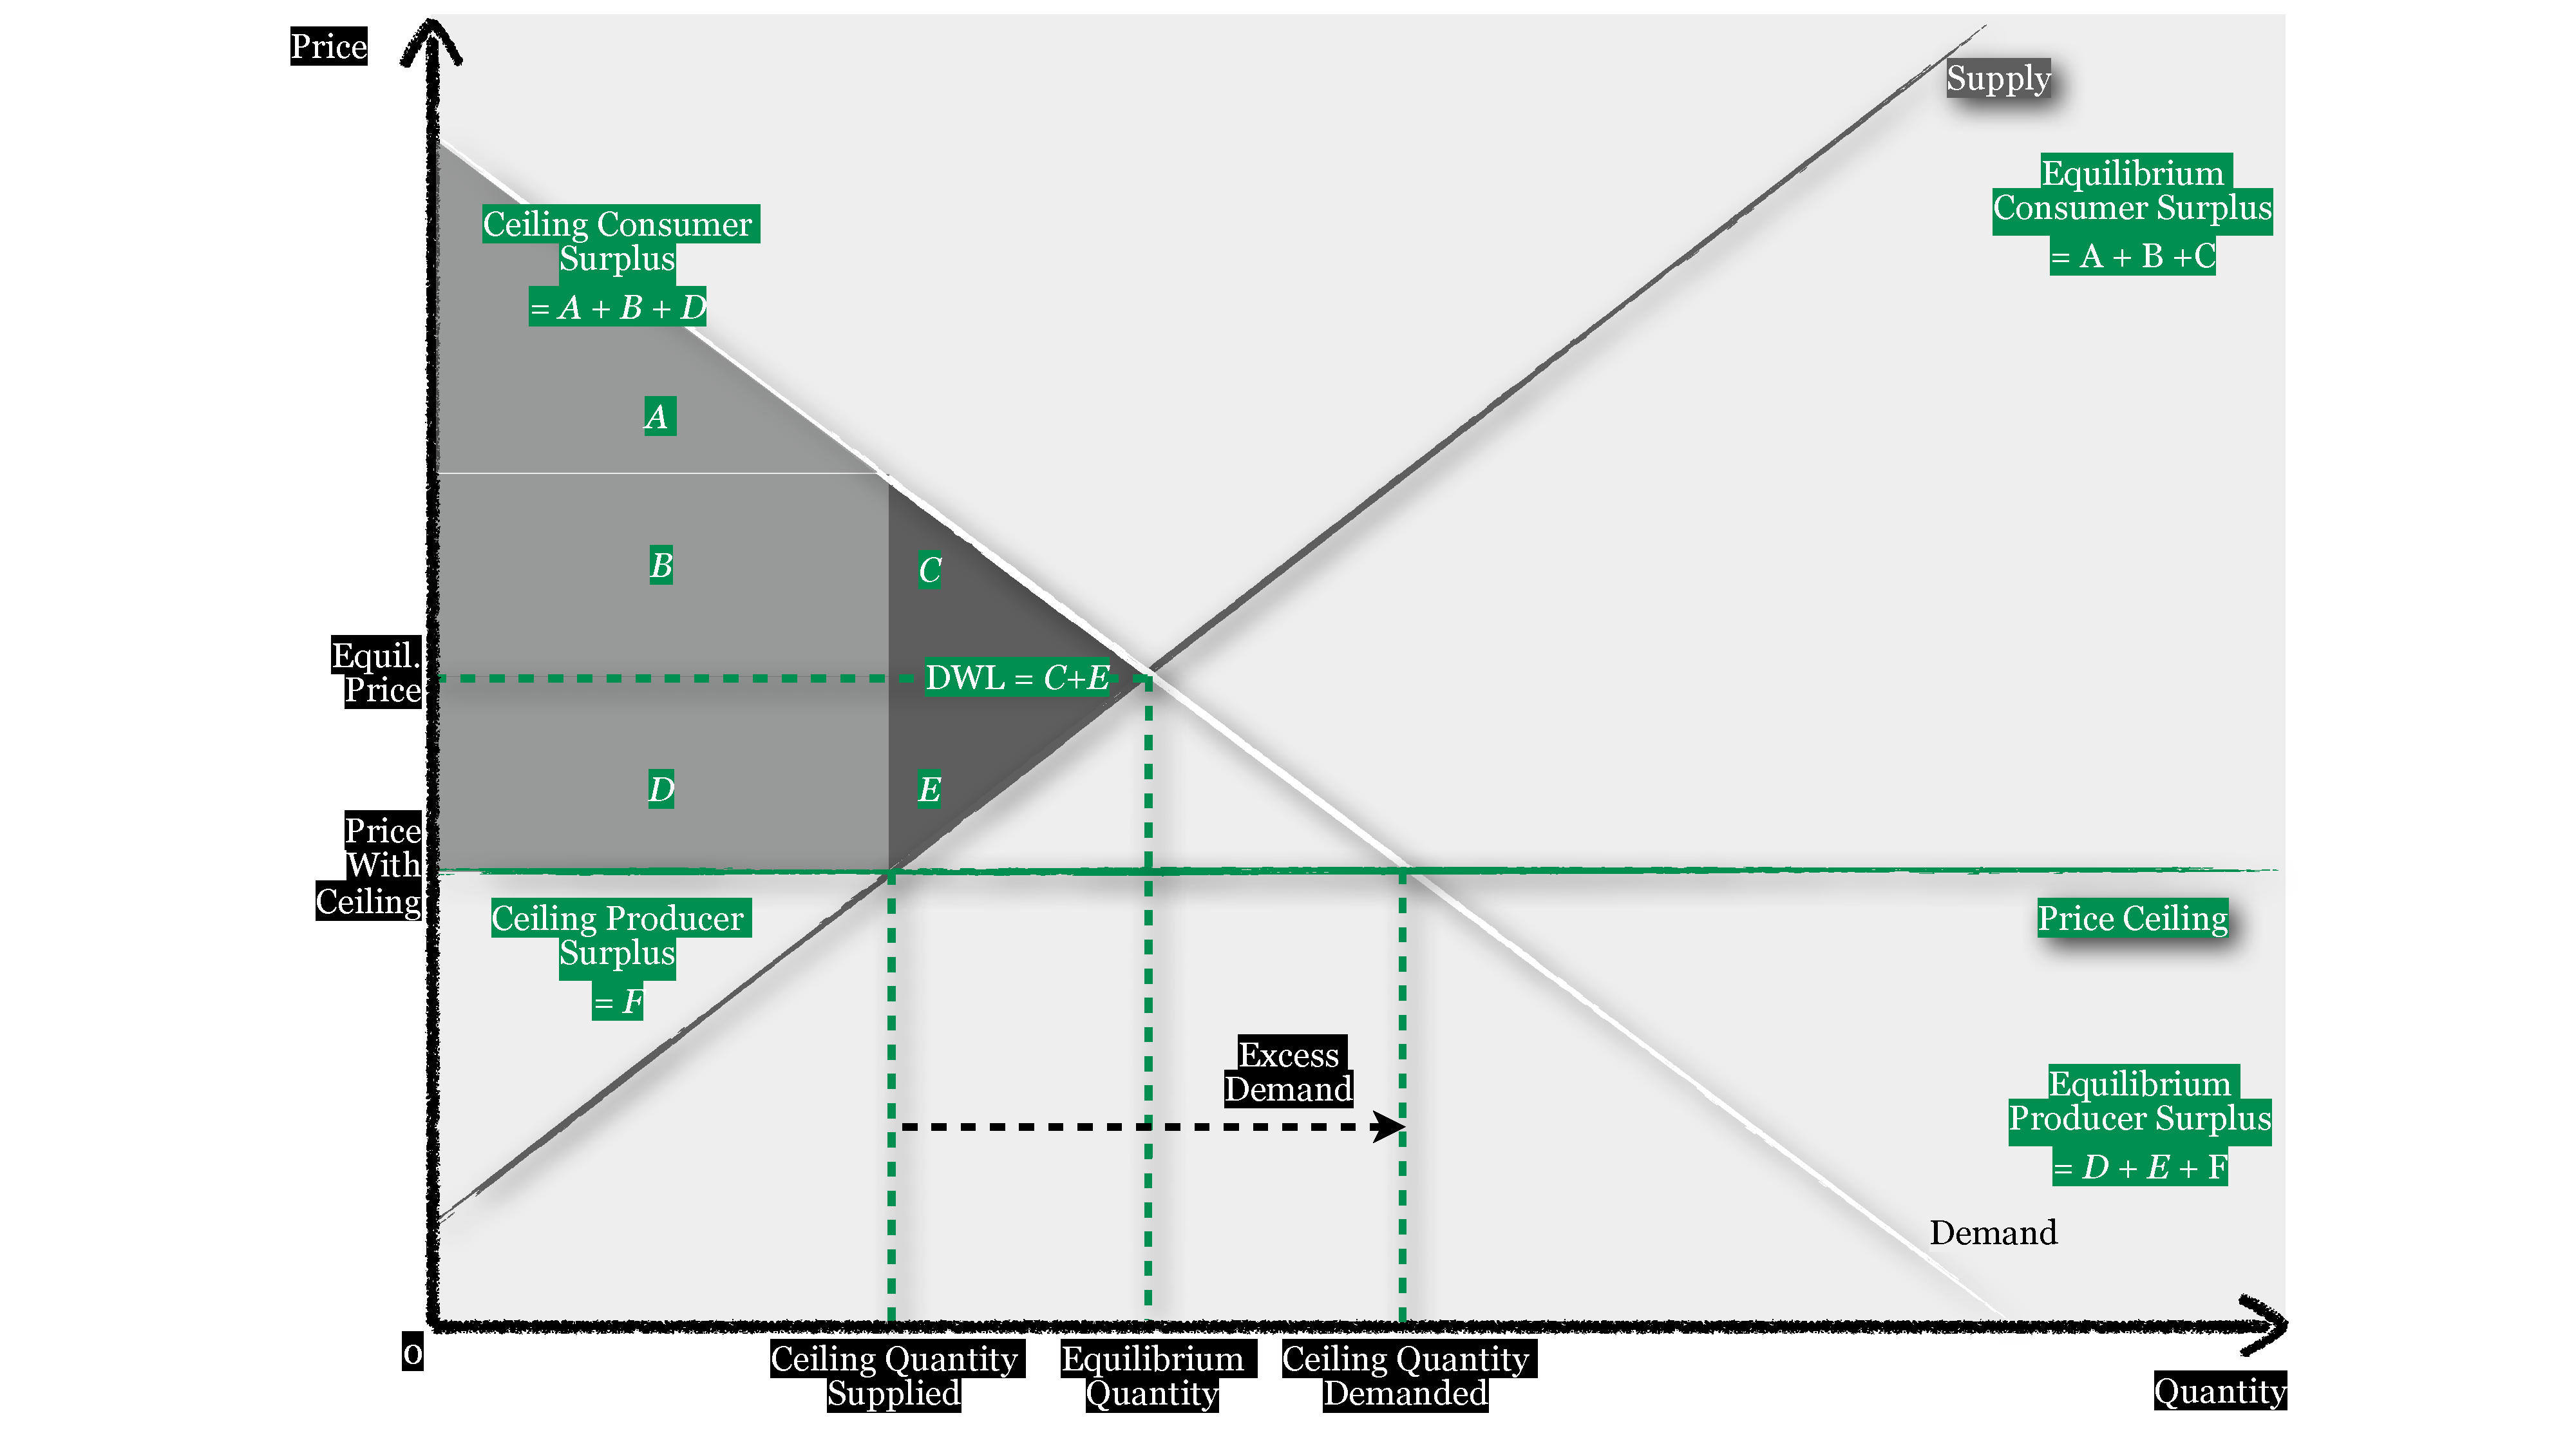
\includegraphics[width=1\textwidth]{./img/price-ceiling}  
	\caption[Efficiency and Equity of a Price Ceiling]{The \gls{DWL} and distributive effects of a price ceiling with unit-elastic demand and supply (e.g. of housing)}	
	\end{center}
	\scriptsize{Compare with \nameref{fig:supplydemand} in figure \ref{fig:supplydemand} (p. \pageref{fig:supplydemand}).}
	\label{fig:price-ceiling}
\end{figure}

\begin{figure}[htbp]
	\begin{center}
	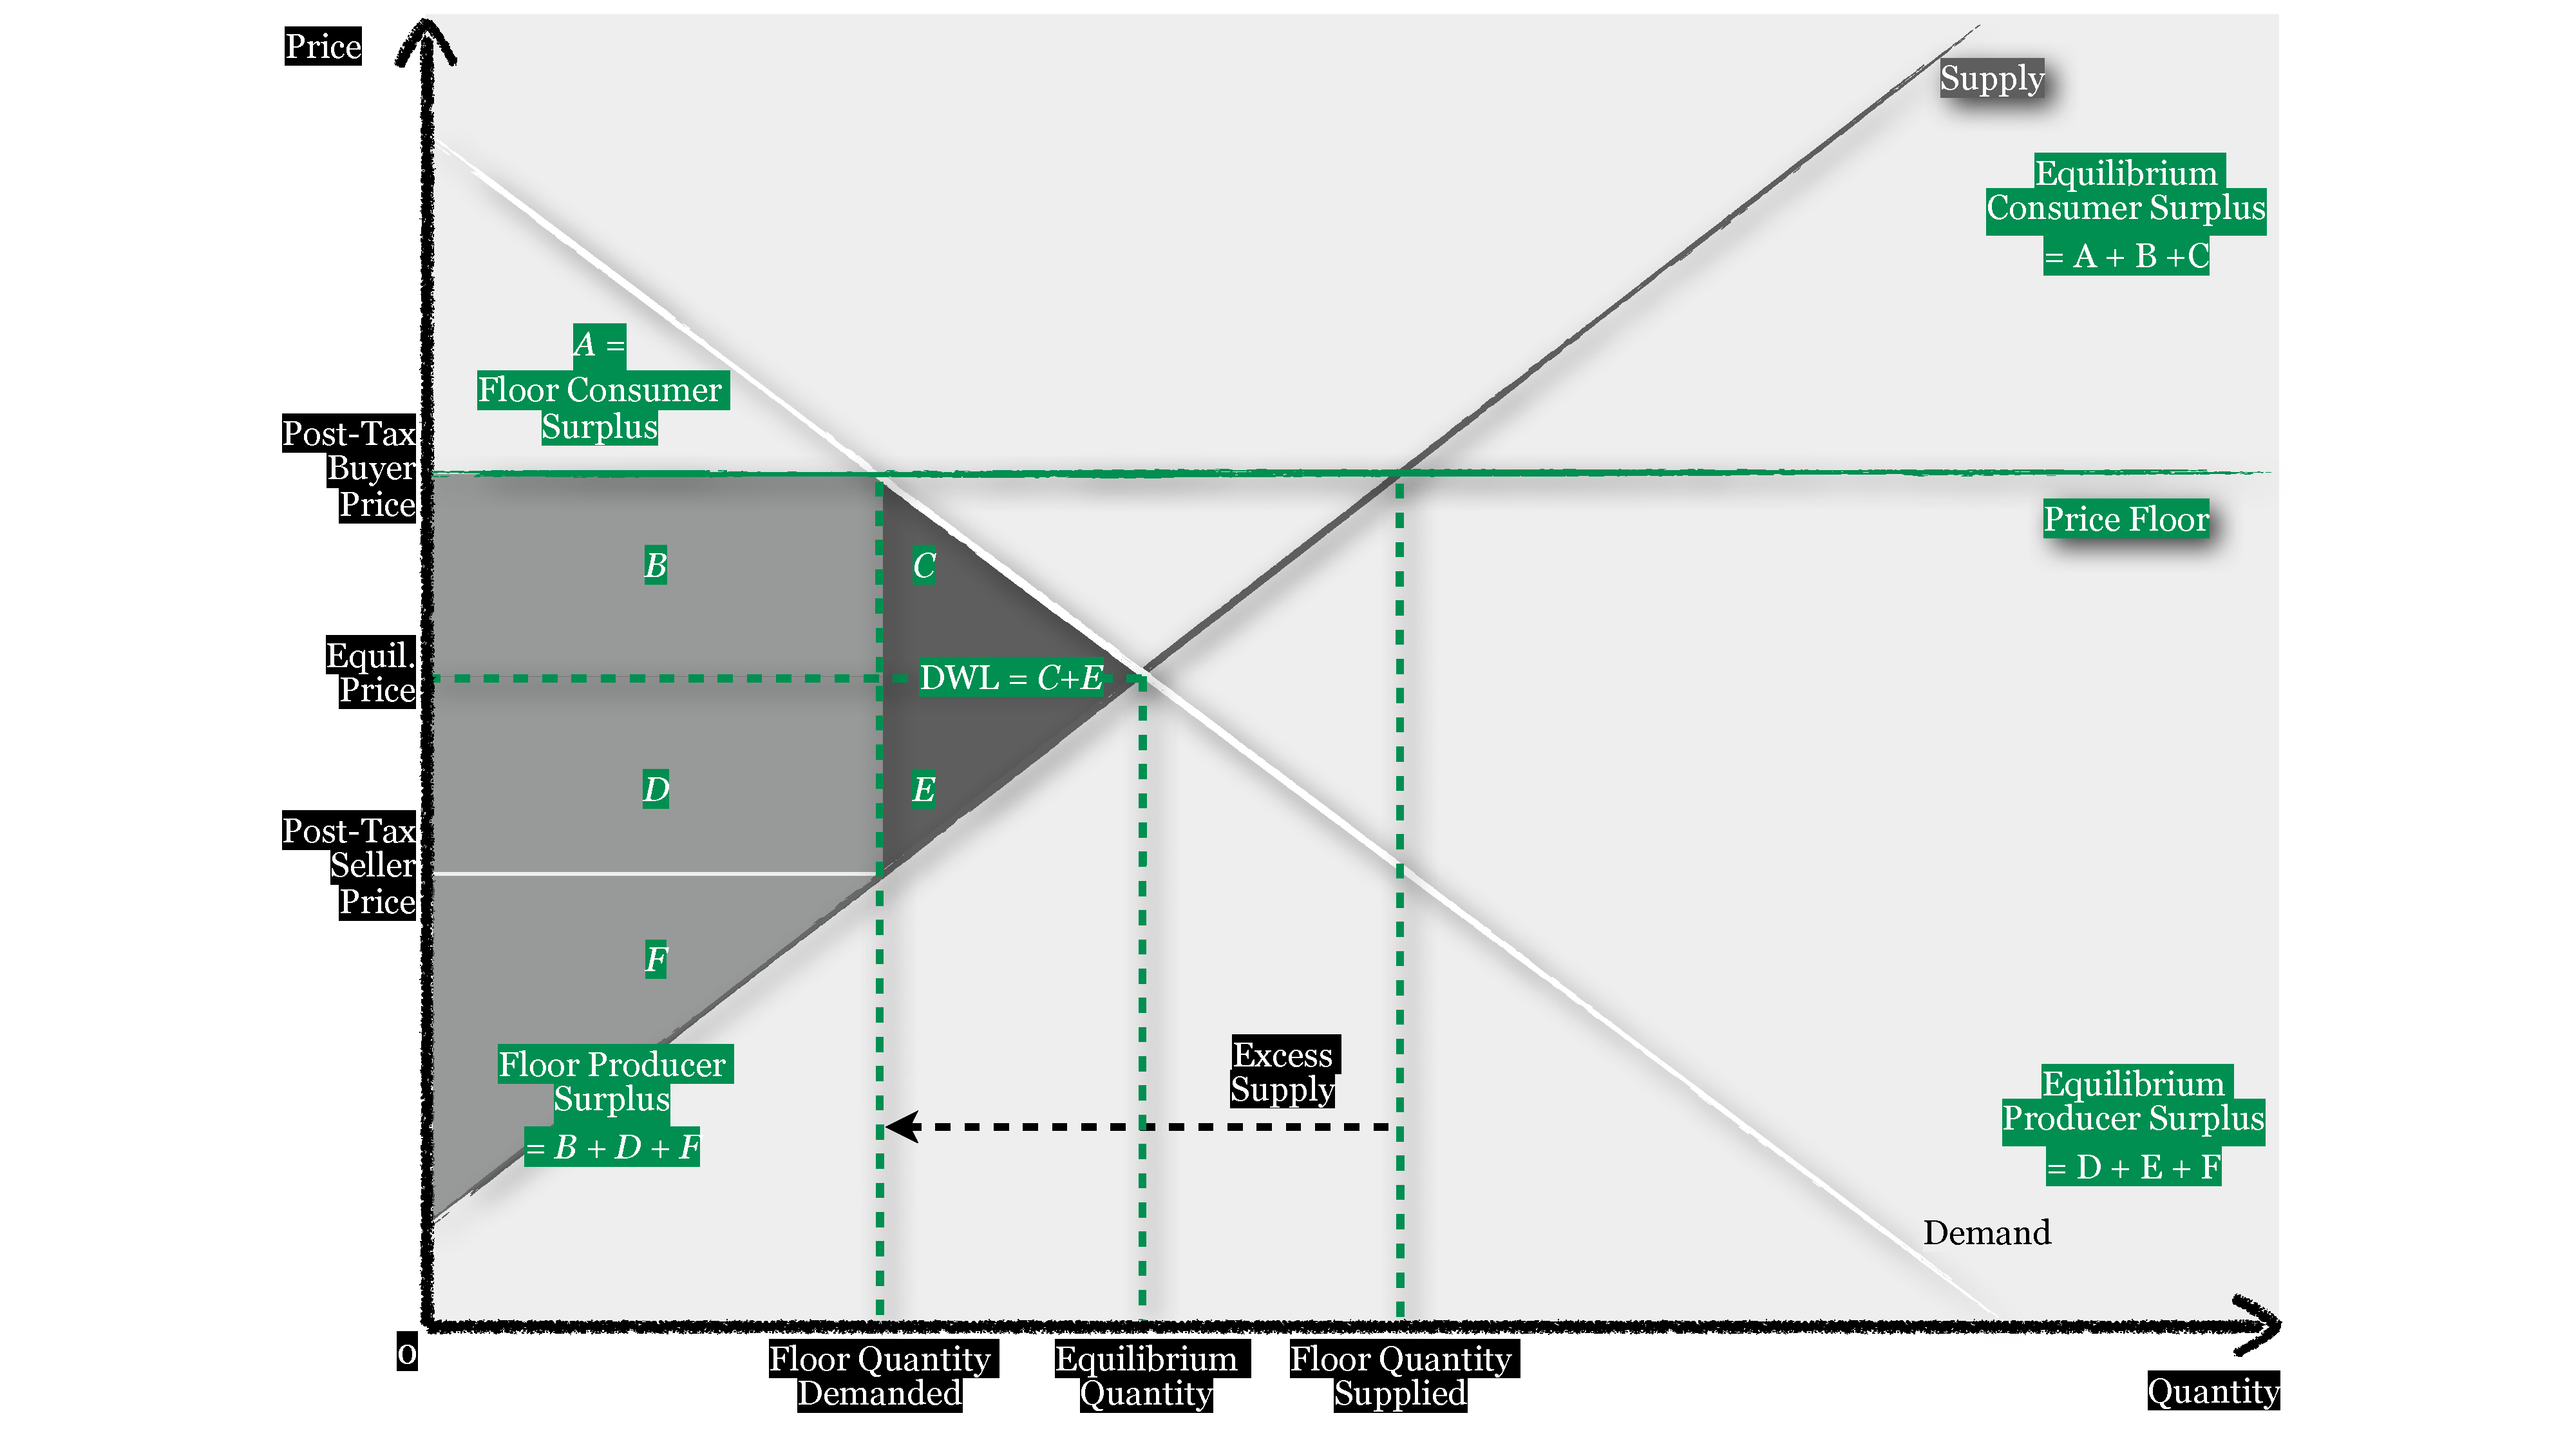
\includegraphics[width=1\textwidth]{./img/price-floor}  
	\caption[Efficiency and Equity of a Price Floor]{The \gls{DWL} and distributive effects of a price floor with unit-elastic demand and supply (e.g. of labor)}
	\end{center}
	\scriptsize{Compare with \nameref{fig:supplydemand} in figure \ref{fig:supplydemand} (p. \pageref{fig:supplydemand}).}
	\label{fig:price-floor}
\end{figure}

\begin{description}
	\item[Efficiency.] 
		In addition to this zero-sum component, price controls also destroy welfare: much like taxes (figure \ref{fig:DWL}), they cause a \gls{DWL}.  Price controls are a negative-sum allocation. Ceilings push prices (say, rents) below equilibrium levels, decrease supply (of flats) and increase demand (for flats), causing excess demand. Some potential tenants cannot find good housing, even though they would be willing to pay a higher rent or some potential landlords will not built or improve housing, even though willing tenants could be found. Conversely, floors push prices (say, wages) above equilibrium levels and increase supply (of labor) and decreases demand (for labor), causing excess supply (unemployment). Some workers cannot find gainful employment, even though they would be willing to work for lower pay or some potential employer will not hire an available worker, because her cost (wage) outweighs her utility (productivity). Under binding price floors, some otherwise pareto-improving exchanges will not be untertaken, causing decrepit real estate\footnote{
			Rent control is famously derided as ``the next best way to destroy a city'' aside from carpet bombing.} 
		or unemployment, respectively. 
	
		The size of the \gls{DWL} of price controls depends on the relative price elasticities of supply and demand (just like the \hyperref[sec:minimalDWL]{\gls{DWL} of taxes}, p. \pageref{sec:minimalDWL}).
		The more price inelastic demand, the smaller is the \gls{DWL} of price floors: even at pushed-up prices, few buyers will be able to exit the market and almost all sellers will find buyers. Conversely, the more price inelastic supply, the smaller is the \gls{DWL} or price ceilings: even at pushed-down prices, few sellers will be able to forego sales and almost all buyers will find sellers. 
	
		In the real world, \hyperref[sec:well-determinedincidence]{elasticity is hard to determine} and depends on many factors (p. \pageref{sec:well-determinedincidence}). 
	
		In housing markets, supply (landlords) may be inelastic in the short run (for existing housing), but very elastic in the long run (for improved, or new housing). \glspl{DWL} (or decrepit housing) are probably sizeable. In labor markets, too, demand (employers) will likely not be price inelastic across the board. Often, labor can be substituted by capital. Here, too, \glspl{DWL} (or unemployment) will be sizeable. In any case, it will be very hard for states to gauge elasticities and calibrate price controls accordingly to specific industries, time periods and regions\footnote{
			In addition to the mere complexity of such regulatory intervention, price controls are also prone to rent-seeking clients. As the gains (and losses) will often be obvious to, and concentrated in some citizens, they may lobby their government to affect changes \citep{Peltzman1976,Posner1975,Krueger1974}. As in oil-rich rentier states \citep{Beblawi1990}, widespread zero-sum games may corrupt politics.}.
		
	\item[Effectiveness.] 
		Price controls are also limited in their effectiveness. They may, in principle --- if at great cost and complexity --- redress the inequities of \nameref{sec:winner-take-all} markets (p. \pageref{sec:winne-take-all}), \nameref{sec:differentbudgetconstraints} (p. \pageref{sec:differentbudgetconstraints}) and \nameref{sec:diminishingmarginalutility} (p. \pageref{sec:diminishingmarginalutility}). Short of a near planned economy, they do little to dampen \nameref{sec:positionalrace}s (p. \pageref{sec:positionalrace}):  consumers can simply buy different (more extravagant) categories of goods, or more of the same to fulfill positional impulses. They can also hardly reign in on \nameref{sec:monopsonyemployers} (p. \pageref{sec:monopsonyemployers}). By definition, their demand for labor is highly price elastic, given plenty of alternatives. Worker supply of labor, absent another employer, is almost perfectly price inelastic. 
\end{description}

Governments should, however, respond to monopsony employers in labor markets either by anti-trust action or by leveling the playing field. Regulating a right to strike\footnote{Such as in Article 9, Section 3 of the German Basic Law.} and the right to form trade unions can put monopoly employees opposite monopsony employers in collective bargaining. Employment protection and labor contract regulation can also alleviate the power imbalance in labor markets.

\subparagraph{Affirmative Action.} \phantomsection \label{sec:affirmativeaction} To a limited extent, governments can also respond to winner-take-all markets with affirmative action or equal opportunity legislation.

\subparagraph{Redistribution by Fiscal Policy} \phantomsection \label{sec:fiscalredistribution} The principal redistributive tool of government is a progressive tax, by which government collects more from the rich to pay for public expenditures, and/or finances handouts to the poor\footnote{
	Unfortunately I cannot discuss the vexing intricacies of tax design here. I review them elsewhere \citep{Held2010a} and argue for a cash-flow based, post-paid \gls{PCT} (recently \citealt{McCaffery2002,McCaffery2005}) and a \gls{LVT} \citep{George1879}, instead of widespread but defunct \gls{PIT} and popular but proportional/regressive \gls{VAT}. If necessary, a \gls{NIT} should be added to fight structural unemployment or working poverty (first suggested by Milton \citealt{Friedman1962}), and a \gls{WT} on net worth to rein in extrem inequity.}
	\footnote{
	Progressive taxation, too, may be unable to mitigate the inequities (and welfare losses) of monopsony employer labor markets. Potentially, monopsony employers will counteract progressive schedules by further lowering their wages.} 
%this seems to be a very, very short section. Maybe expand or refer to other section?
%alternative footnote %\footnote{See later chapter on tax.}%bad footnote, this replaces the EU original footnote

\subparagraph{Redistribution by Monetary Policy} \phantomsection \label{sec:distributive-effects-of-inflation}.  Monetary policy cannot effectively mitigate inequitable market outcomes. Inflation and deflation redistribute wealth, but not between the rich and the poor. Instead, inflation redistributes wealth between credits denominated in real terms (e.g. house ownership), debts denominated in nominal terms (e.g. a fixed-rate mortgage) and credits denominated in nominal terms (e.g. fixed-rate pension) and debts denominated in debts denominated in real terms (e.g. a futures contract) as summarized in figure \ref{fig:distributive-effects-of-inflation}. 

\begin{figure}[htbp]
	\centering
	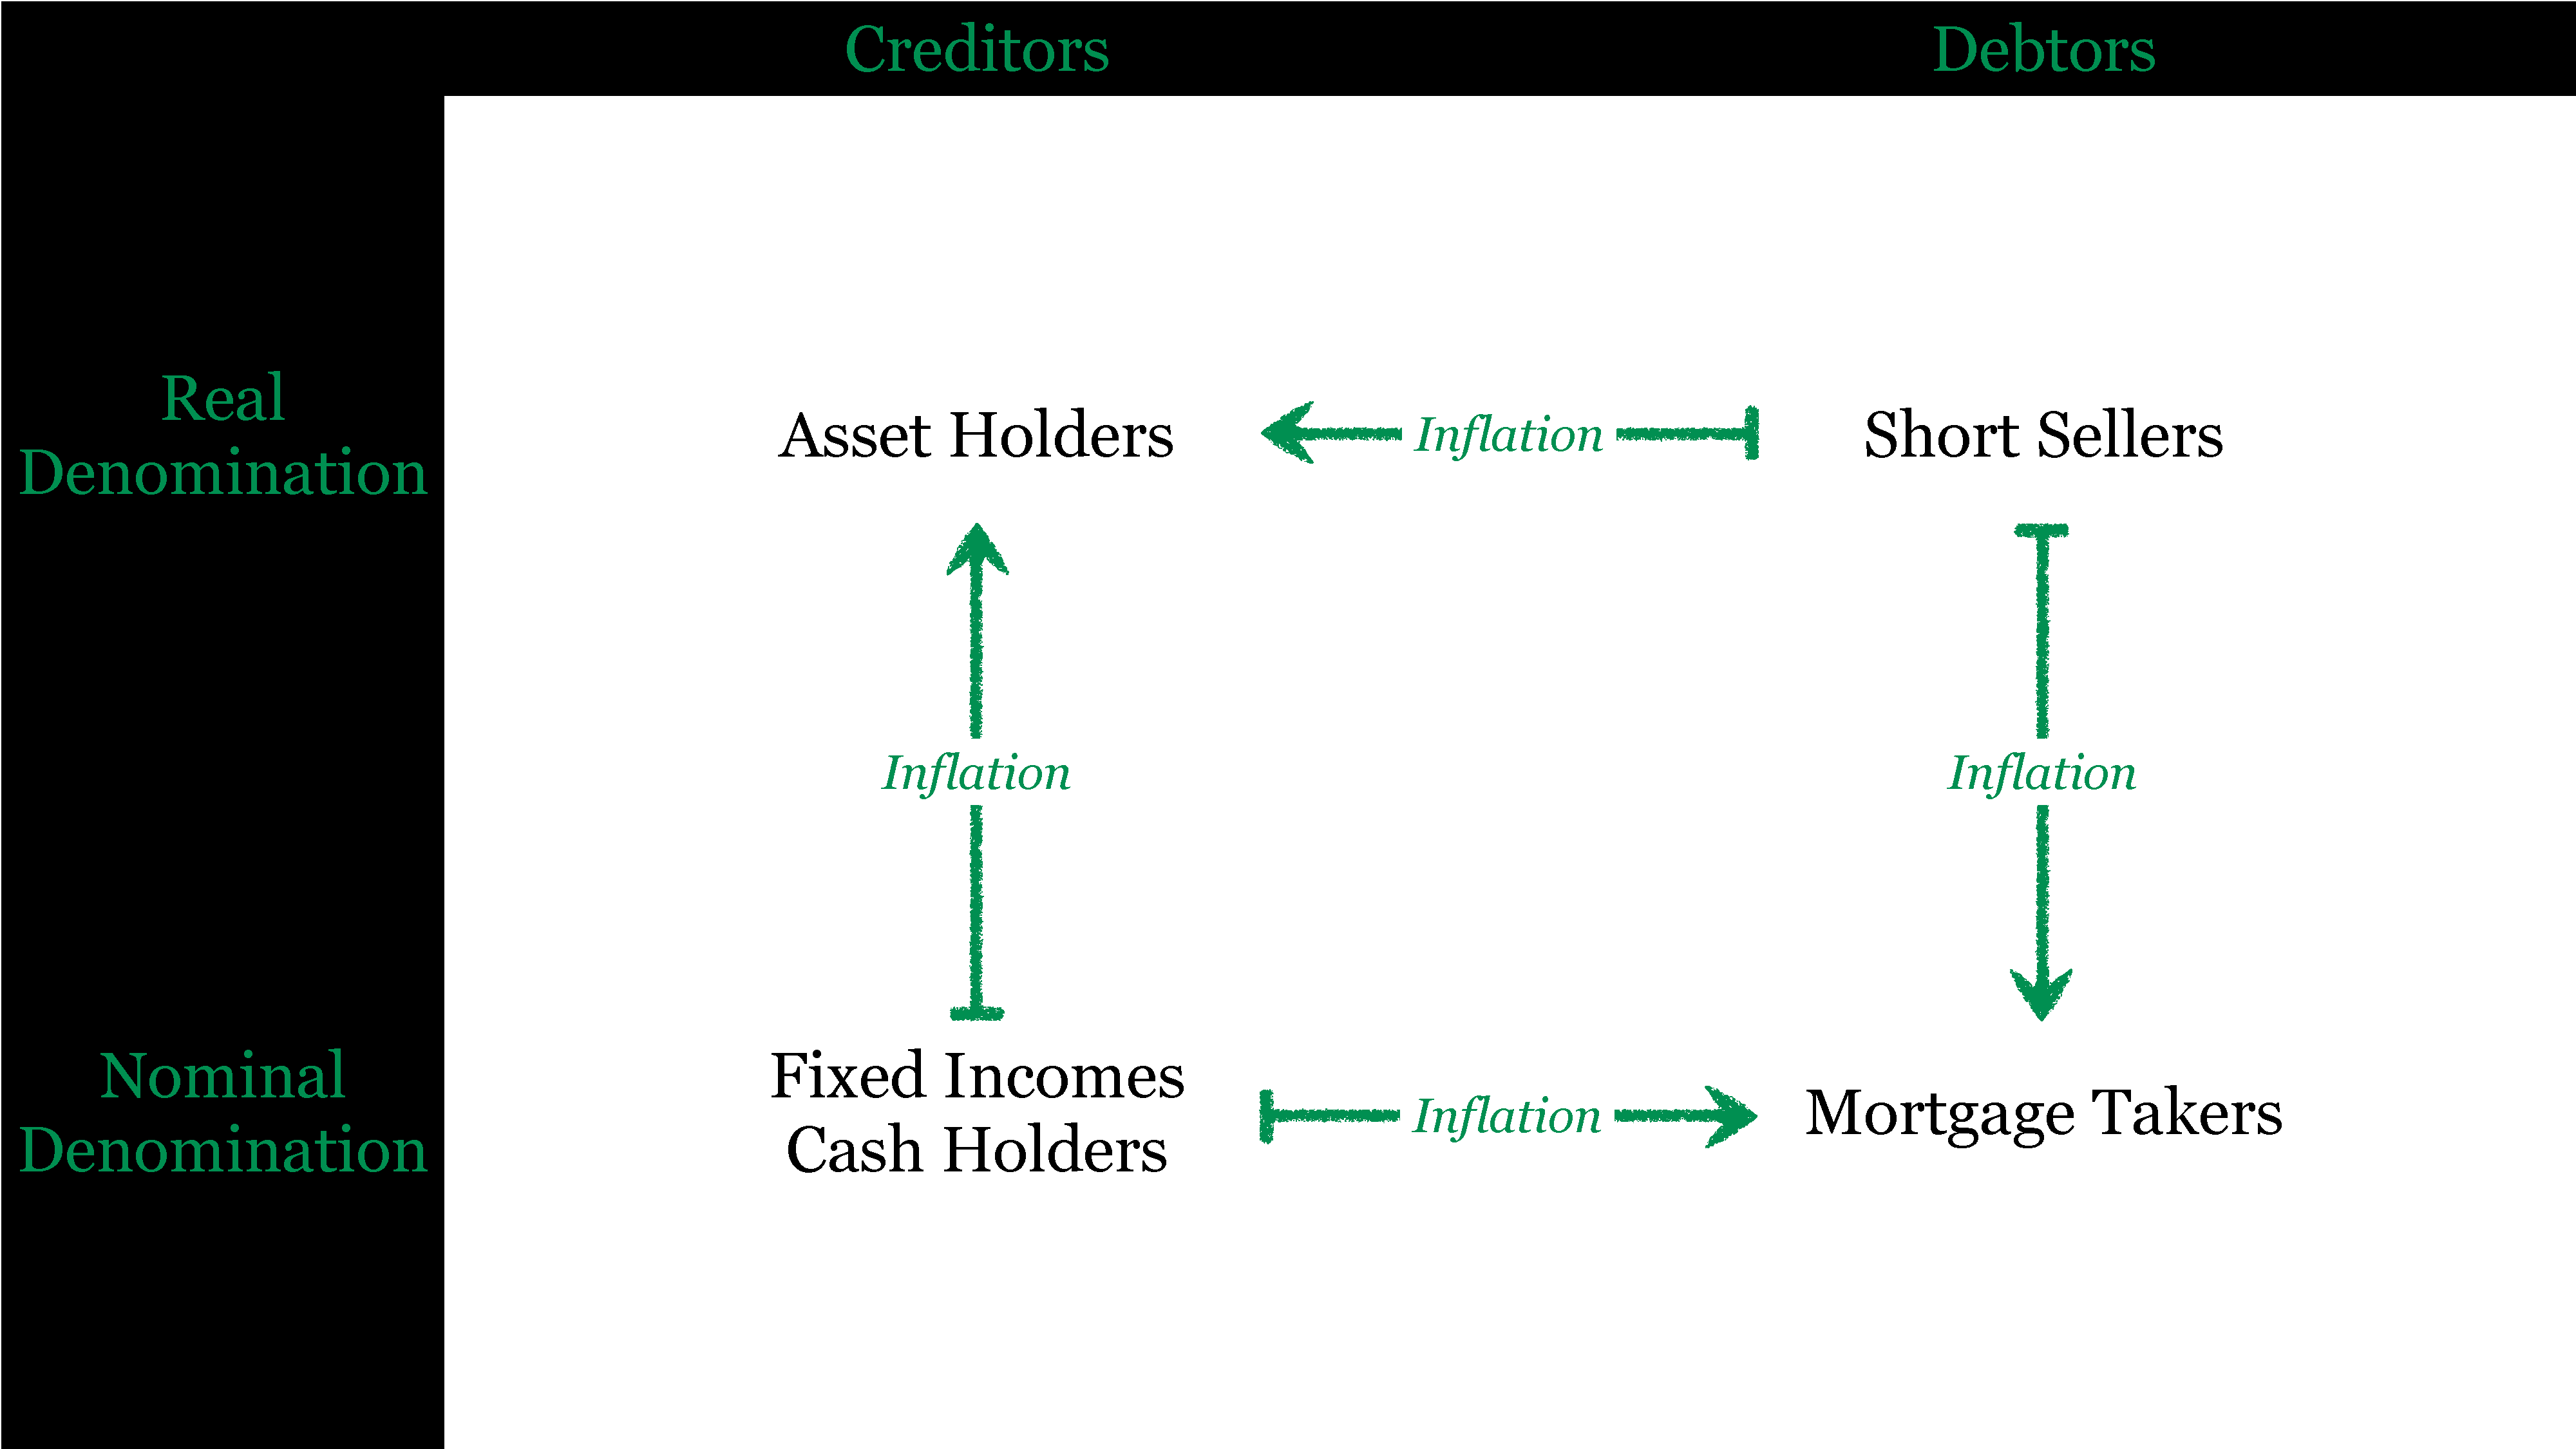
\includegraphics[width=1\textwidth]{./img/distributive-effects-of-inflation}  
	\caption[Distributive Effects of Inflation]{The distributive effects of inflation, with some examples}
	\label{fig:distributive-effects-of-inflation}
\end{figure}

Such arbitrary redistribution does not correspond to \nameref{sec:inequalitydynamics} of markets  (p.\pageref{sec:inequalitydynamics}) and cannot be defended on normative grounds\footnote{
	Rich people are more likely to be creditors, and poor people more likely to be debtors. Telling, as \cite{Coggan2011} does, the history of mankind as the struggle between debtors and creditors (paraphrasing \citealt{Marx-1867-aa}) may be roughly adequate and enlightening, but the simplification carries only so far. As \citeauthor{Coggan2011}(\citeyear{Coggan2011}: loc 6-24-04) himself points out, German hyperinflation wiped out the (often nominally denominated) savings of the middle class, but left relatively unaffected the (often real denominated) wealth of the upper class and the subsisting lower class with neither debt nor savings.}. 
	
Additionally, redistributing by monetary policy causes severe \hyperref[sec:pricestability]{welfare losses} (p. \pageref{sec:pricestability}. Today, as financial products have diversified, redistributing based on denomination and between creditors and debtors will have increasingly arbitrary results\footnote{
	There is a case to be made for deliberately sharing the burden of systemic and unsustainably high levels of debt, as may be case with Greek sovereign debt in the 2007ff financial crisis \citep{Coggan2011}. As \citeauthor{Coggan2011} reminds us, we do not need inflation to achieve that; a (partial) default will do the trick, colloquially referred to as a ``haircut'' in the 2007ff financial crisis.}.

Monetary policy on distributive goals, as on \nameref{sec:production} (p.\pageref{sec:production}), shines by staying neutral. It must strive to maintain price stability to avoid any arbitrary and undue distributive effects that would otherwise interfere with the distributive dynamics of state and market.

\subsubsection[Consistency Over Time]{Consistency Over Time: Saving Tomorrow's Pie}\label{sec:time} 

\begin{quote}
\emph{``Give me chastity and continence, but not yet.''\\}
--- \citeauthor{St.AugusteofHippo397} Confessions (VIII, 7)
\end{quote}

\paragraph{The Human Condition in Time}
Human beings are myopic planners \citep{Kahneman47}. They discount the future hyberbolically; the more remote a future event is, the more humans discount its rewards (\citealt{Ainslie1975}, \citealt{Thaler1981}). Human beings also succumb to herding: they do as others around them do. %citation needed. 
Both these frailties can lead to time inconsistency, where we simultaneously hold incompatible preferences for our present and future selves, for example when we would like to retire somewhere warm and mild, but also want a new car every three years.

To be time consistent, we have to do unto future generations (or selves) as we would have them do unto us (the Golden Rule of reciprocity). Applied to the material world, we have to save --- at least --- at that level, which allows the highest constant level of current and future consumption (\citealt{Phelps1966a}, \citealt{Solow1956}). If we are more generous to our children, or consider technological innovation to be endogenous, we might have to save even more.

Time consistency bears both on equity and efficiency. An \emph{equitable} policy ensures same (discounted\footnote{
	\label{fn:3components}In his treatise on the economic costs of global warming, \citeauthor{Stern-2006-aa} lists three components to discount to future utility. \begin{inparaenum}[\itshape 1\upshape)] 
		\item future people may value an additional unit of consumption less (or more) if they have more (or less) output available overall (elasticity of marginal utility). 
		\item expected but \emph{exogenous} growth, such as a chance discovery of a new technology, may increase future output without requiring present people to give up anything. 
		\item people will discount future utility simply because it is in the future and uncertain (the pure discount rate of the future) (\citeyear{Stern-2006-aa}: 52).
	\end{inparaenum}})
utility for people living today vs. people living in the future. An \emph{efficient} policy ensures maximum (discounted) growth over all periods (along the long-term growth path of the economy). %needs citation, adequate terminology. 

%Where does this belong?!? 
	%big ass comparison on public finance (not exactly sure): There are stocks (equity) and bonds (debt) markets for private financial markets. The public equivalent is tax (like equity) and govm debt (like debt).

\paragraph{Interest} \phantomsection \label{sec:interest} In the exchange economy, capital markets align preferences of present and future generations (and selves) by compensating savers with an interest. Ideally, risk-free\footnote{
	Idiosyncratic risk of specific investments are diversified or hedged away. Risk-free interest rates still include a premium for \emph{systematic} (not systemic) or aggregate risk, such as the continued existence of life on earth. The remaining interest component, the pure discounting of future utility, represents the hedonic loss of present, myopic individuals.} 
interest rates, and other (hedged) returns on capital (e.g. stock market indices) equilibrate at that level, where future marginal utility equals present marginal cost of saving. At this intertemporal optimum\footnote{
	Specifically, saving (below \citeauthor{Solow1956}'s optimal rate) without interest is a \citeauthor{Kaldor1939}-\citeauthor{Hicks1939} improvement: future utility is greater than present cost. Interest can be considered an intertemporal sidepayment from the future to the present. With interest, sub-optimal level saving can be pareto improved: upon saving more, both present and future generations (and selves) are at least equally well off.}, 
we follow the Golden Rule: present generations (and selves) \emph{do} unto future generations (and selves) as vice versa. 

Under the assumptions of (neo)classical orthodoxy, efficient capital markets should guarantee \emph{some} degree of time consistency. 

\subparagraph{Garbage In, Garbage Out.} But because markets are ultimately \emph{aimless} and operate on (assumed!) \emph{exogenous} preferences, the \emph{formal} ability of capital markets for intertemporal optimization is strictly limited. Interest rates --- as all other prices --- are elegantly aggregated (time) preferences of people. If these preferences are inconsistent suggest), or amoral, so, too, will be the resulting market ``optimum''. As in statistical analyses, no matter the algorithm, the quality of the output depends strictly on the quality of the inputs.

People may be relatively consistent or at least our best bet to gauge some components of observed discount rates, including the likelihood of exogenous growth (innovation), or continued human existence (compare footnote \ref{fn:3components} (p. \pageref{fn:3components}). For these components, people may input reasonably good `data`, and markets will output reasonably good prices.

By contrast, the `data quality` of \emph{pure discount component rate of the future} --- discounting future utility simply because it lies in the future --- is deeply questionable for reasons (compare footnote \ref{fn:3components} (p. \pageref{fn:3components}):

\begin{enumerate}
	\item \emph{Inconsistency.} People are, as cognitive psychology has shown, \emph{time inconsistent} even in their own lives, and the short- to medium term (\citealt{Ainslie1975}, \citealt{Thaler1981}). If they are similarly inconsistent  when deciding how much to saving to supply at any given interest rate, \emph{overall} interest rates will be distorted. Myopic individuals will \emph{cause} the very inflated interest rates meant to keep their short-sightedness in check, and overall saving will be too low\footnote{
		Myopia implies a shift in the supply curve of saving. For any given interest rate, people will supply less.}.
	\item \emph{Morality.} As \citeauthor{Samuelson2005} (\citeyear{Samuelson2005}: 54 as cited in \citealt{Stern-2006-aa}) has recently reminded us, term uncertainty, especially pure discounting of the future is a normative concern. Just how much we value the welfare of future generations and selves is a \emph{moral} judgement. There is nothing in our nature or our environment that could positively tell us what a \emph{true} rate would be, there are only normative judgments of what a \emph{right} rate should be. Once people have agreed on such a rate, markets can do the number crunching. But markets, because they will accept \emph{any} rate as input, cannot solve this moral problem for us. Instead, only a democratic polity --- and its government --- can decide the pure discount rate.
		
	People often say they want their children to live a better life. If similar sentiments are deeply-held and widespread, people might democratically decide to save more than intertemporal \emph{equity} demands. If indeed, we shall give to our children \emph{better}, than we ourselves received, we are at least looking for a \emph{Kaldor-Hicks} (not Pareto!) improvement without and above the equilibrium capital return.
	
\end{enumerate}

Even ignoring such substantive concerns, real world capital markets are also plagued by \emph{formal} intertemporal failures, causing their own costly and inequitable time inconsistency. The capitalist algorithm not only receives bad inputs, but it is also ridden with bugs, that fail both in the short and the long term.

\paragraph{Short-Term Intertemporal Failures} \label{sec:short-terminconsistency} Economic activity tends to fluctuate in the short-term. 

\subparagraph{Business cycles} are periodic fluctuations, typically relatively mild in amplitude and slope. They endogenously caused by lumpy, lagged decision-making of market participants, for example in inventory cycles\footnote{
	\emph{Endogenous} business cycle durations range from 3--5 years for lagged inventory decisions \citep{Kitchin1923}, 7--11 for fixed investment \citep{Juglar1862}, 15--25 for infrastructural investment \citep{Kuznets1930} and 45-60 for technological revolutions \citep{Kondratiev1925}. \\ For a recent empirical test of all four business cycle theories, see \cite{Korotayev2010}. \\ The latter two of these are probably beyond reliable anticipation and certainly beyond the short-term. They are also contested as empirical artifacts \citep{Howrey1968} or restricted to heterodox, evolutionary economics \citep{Modelski2010}.}.

According to the dissenting, minority view, business cycles are \emph{true} shocks that may or may not be endogenously amplified, but are exogenous in origin (\citealt{Kydland1982})\footnote{
	\gls{RBCT} proponents consequently argue against state interventions to counteract these exogenous shocks.}.

\subparagraph{Bubbles and panics} can lead to abrupt and dramatic fluctuations in economic activity, with great slope and amplitude. Bubbles and panics envelope market actors when they make their decisions based on the anticipated decisions of others, in a beauty-contest type game \citep{Keynes1936}. Similar rationales also emerge when making privately informed decisions creates a positive externality for other participants to free-ride on your inadvertently disclosed information \citep{Banerjee-1992-aa}\footnote{
	For a fully-fledged account, involving the debt, equity and asset market as well as monetary and regulatory correlates of \emph{Maniacs, Panics and Crashes}, see \cite{KindlebergerAliber-2005-aa}. Herding has also been complemented and expanded into the (heterodox) debt-deflation theory of economic cycles, where credit cycles magnify initial bubbles, panics or shocks \citep{Fisher1933}.}.

\subparagraph{Fluctuations are Costly.} Both types of fluctuations in economic activity are inefficient because they temporarily leave factors of production idle (overused) and increase periodic transaction costs. Fluctuations  leave factors of production (for example, an assembly line) idle during the downturn or building up excess capacities during the upturn (for example, a real estate overhang). Additionally, fluctuations cause unnecessary adjustment costs (for example, storing equipment). The costs of short-term fluctuations are particularly virulent in labor markets, where hiring is expensive and unemployment can degrade worker morale. Aside from these material costs, short-term and uncertain employment (and economic prospects in general) cause stress and hardship. %this needs a source

Such idleness or mania diverts the economy away from its (exogenously) long-term growth path and thereby slows down the economies progress along the growth path.

By contrast, ``true'' exogenous shocks (such as an earthquake) or genuinely new information about future utility of present savings (for example, because of a new technology) is not a deviation from, but a \emph{shift} in the long-term growth path. It is, for better or for worse, unavoidable.

\paragraph{Short-term: State responses}
States can respond by regulatory, fiscal and monetary means to reduce the frequency, depth and duration of economic fluctuations. In the following, I discuss the state responses to a downward deviation from the long-term growth path of the economy. States should likewise, if with opposite sign, respond to upward deviations from long-term growth.

\subparagraph{Regulatory}
States can reign in on short-term downturns simply by outlawing respective actions of market participants. \gls{EPL}, for example, can include lay-off protection, making it harder for employers to fire workers in a downturn. Other regulatory interventions include the bans on short-selling of recent 2007ff fame. %maybe discuss decommodification again, here. Why does this, or does this not, belong in here? I think decommodification is a second-order consideration, that's why it doesn't belong in here.

Regulatory responses can be effective, but blunt instruments as they also affect economic activity outside of endogenous downturns. Generous lay-off protection, for instance, can cause a \gls{DWL} of unemployment during upturns, keeping the economy under its long-term growth path. Regulatory interventions can also fail to distinguish between endogenous and exogenous fluctuations in the economy overall and some of its markets\footnote{
	Generous lay-off protection has been hypothesized to contribute to ``eurosclerosis''.}. %citation, explanation needed 
As collateral damage, generous lay-off protection may prevent workers from moving to new, more productive firms and sectors (for example services rather than mining). Similarly, bans on short-selling may prevent or defer necessary market readjustment in case of real, exogenous price shocks (for example, a war in an oil-exporting country).

\subparagraph{Fiscal Stimulus.} \phantomsection \label{sec:fiscalstimulus}
States can also respond to short-term downturns by propping up aggregate demand, following \citeauthor{Keynes1936}ian demand management \footnote{
	According to the opposing, now minority view of \gls{RET}, fiscal expansion will be ineffective, because market participants will correctly anticipate that current deficit spending (expansion) will be offset by future tax hikes (contraction). Anticipating such future losses, they will hoard more cash and equivalents today, than they would otherwise, thereby negating any current period effect.\\ Even though controlled experiments are not readily available at the level of entire economies, deficit spending seems to work, at least a little. Here, for once, human ignorance (of \gls{RET}) is not only bliss, but also a blessing for all of us.}.

By definition, to push up aggregate demand, government must dissave. Fiscal stimulus must be paid out of newly issued debt, or prior savings --- but it cannot be paid out of increased \emph{current} period tax revenues, for such hikes would cut private demand, as public demand expands\footnote{
	A democratic polity can \hyperref[sec:tradeoffs]{trade off} public for private demand as it wishes (p. \pageref{sec:tradeoffs}), but any such balance will not affect aggregate (public \emph{and} private) demand. Democracies can call this shot, but it will not alleviate slumps.}. 
Still, even \emph{deficit spending} will \emph{crowd out} private demand, as it soaks up savings in capital markets. Government bonds must be sold to someone, and that someone will not be able to spend or invest that same money elsewhere.

Luckily for government (and all of us), it can target its spending wisely to those areas where it will have a maximum \emph{multiplier effect}, that is, where demand begets as much more demand as possible. For example, when government procures a new railroad line, these construction workers will have more resources to spend on entertainment, or invest in a family home. Government demand is not the only demand that multiplies; private demand also does. However, because government (ideally) aims not to maximize individual profits, but overall economic recovery, it can seek out that spending that maximizes multiplication. Private demand, by contrast, will seek maximum profit at low risk, which, in economic downturns, is often found in a ``flight to safety'', hoarding of cash or equivalents.

A good stabilizer should go entirely into immediate consumption or investment, and possibly incentivize further dissaving\footnote{
	The 2009 \emph{cash-for-clunkers} scheme --- for all its infamous waste, cannibalizing effects and blatant clientelism --- included such an incentive: car buyers had to top-up the subsidy with own savings to buy a new car.}.

While easier to understand for the often maligned deficit spending type of stimulus, governments must trade off the multiplication effect versus the crowding out effect during \emph{all} fiscal expansions. Even when (or rather, hypothetically, \emph{if}) governments were to pay for stimulus ``out of pocket'', these now dispersed savings were collected at an earlier time, ever since they crowded out that same amount in private demand.

Maximizing multiplied demand, for every increment of demand crowded out is a challenge that government must always face in fiscal expansion. Where to best direct resources is an empirical question for econometricians, statistical physicists and other experts that I happily need not, and cannot engage here. 
	
\emph{Automatic stabilizers} can support demand without legislative intervention. They include unemployment insurance\footnote{
	To the extent that it serves as an automatic stabilizer and/or pools the near-universal risk of unemployment, ``unemployment insurance'' is, again, a misnomer. Unemployment benefits are a public good, idiosyncratically financed out of a specific tax in many countries.} %add respective footnote, i talk about this somewhere else. %This isn't quite right yet. Check desideratum from MPP RedistributionAndRevenueAreOne 
and short-time working benefits, both of which smooth out (consumer) demand by substituting the market income of laid-off, or shorted workers\footnote{
	(German) automatic stabilizers have recently faired well during the 2007ff financial crisis and received great praise by \glspl{IFI} (\citealt{IMF-2008-ab}: 20, \citealt{WorldBank2008}: 19) and experts (\citealt{BofingerFranz-2007-aa}: 8).}. 

\emph{Discretionary stabilizers} are often called for when bubbles, panics or amplified shocks cause output fluctuations too large and fast to be captured by automatic stabilizers. They come in the form of tax breaks, stimulus subsidies or public investment. They, too, rely on dissaving, and the incurred debt must be repaid in good times. 

\emph{Side effects.} As all potent drugs, fiscal stimulus must be prescribed with great care. It has at least two dangerous side effects:
\begin{enumerate}
	\item \emph{Structural painkiller.} All stabilizers can disguise real needs for adjustment as cyclical problems, further diverting an economy from its equilibrium and long-term growth path.  
	\item \emph{Playing favors.} Especially discretionary stabilizers are also prone to clientelism, that easily creeps in when legislatures pass often very targeted stimulus packages. When specific decisions are made, rather than general rules passed \citep{Weber-1918-aa}, as discretionary stabilizers require, special interests are more likely to gain the upper hand\footnote{
		The 2009 VAT break handed out to the hospitality sector by the new liberal-conservative coalition in Germany is a recent, brazen example.}.
\end{enumerate}

\subparagraph{Monetary Stimulus.} \phantomsection \label{sec:monetarystimulus}
Government can also prop up the economy in the short run by monetary stimulus\footnote{
	Technically, central banks can lower the (federal funds) interest rate by buying (back) government bonds (\emph{\gls{OMO}}), pump cash in the economy by buying assets (\glsfirst{QE}) or accept riskier collateral from commercial banks (\emph{qualitative easing} \citep{Buiter2008}).}. 
Government injects more cash into the economy, to make up for liquidity frozen up during the downturn, thereby \hyperref[sec:pricestability]{holding the money supply \emph{constant}} (p. \pageref{sec:pricestability})\footnote{
	``Monetary expansion'' is thereby a misnomer.}.

The monetary contraction in the course of an endogenous downturn can best be described as a general loss of confidence in the profitability of future projects (such as investments). As market participants become squeamish about economic prospects in general, they hoard cash (or equivalents) or flee to safety (such as gold, or --- before 2009 --- government bonds)\footnote{
	This is the (Post-)Keynesian consensus. Strict monetarists argue that the money supply \emph{always} remains at equilibrium without government intervention.}. 
Less funding is available even for the most profitable and risk-free projects and the lack of liquidity can render (balance sheet) solvent firms (cash flow) insolvent. The money supply contracts. When these defaults further feed the market panic and cause more debts to sour, a self-reinforcing debt-deflation crises may ensue. %add citation

A monetary stimulus bolsters market confidence by essentially placing an optimistic, massively government-backed bet. When central banks resort to quantitative or qualitative easing, they declare whichever assets they buy or collateral they accept as worthwhile (profitable) investments by fiat. When, if and to the extent that markets buy into this stunt of optimism, they will be increasingly willing to lend the injected (and their own) money again, too.

Monetary stimulus has some drawbacks, too. Monitoring the money supply in the economy is very difficult and imprecise, and related policy imperatives are incompletely understood. To avoid inflation, central banks must contract their money supply again as soon as the monetary stimulus has worked, and market liquidity has recovered. The timing and calibration of interventions to maintain a constant money supply are crucial, but difficult to get right. 

Monetary stimulus, too, can disguise and defer unavoidable realignment when the cause of the downturn is exogenous, such as a true price shock (as for example when revised Greek fiscal numbers became available in 2008). When the long-term growth path is shifted (downward), the money supply \emph{must} contract in absolute terms as the underlying economy, too, will contract, or at least grow slower than previously expected. Monetary stimulus does not allow economies to live beyond their real, exogenous means for long; it just defers the pain to a later contraction or risks inflation, which in turn \hyperref[sec:distributive-effects-of-inflation]{. distributes the costs of realignment arbitrarily} (p. \pageref{sec:distributive-effects-of-inflation}. 

%this needs to be further tied in with the general section explaining money. 
	% not sure where such a section would be, do I really need it?
	%It really doesn’t much matter which kind of inflation targeting you’re using here. 
	%Actually think again about that. You mind need constant money supply.

\paragraph{Long-Term Inconsistency} \label{sec:long-terminconsistency}

\subparagraph{Market problems} The market institution of equilibrium interest rates may fail to guide humans to temporal consistency in the long run for three reasons.

\begin{enumerate}%I think I need to introduce Solow before this ...
	\item (Exogenous) growth theory discussed so far assumes technology to be constant, or exogenous: as if the rate at which new technology is discovered cannot be altered by humans. Accordingly, once a maximum steady-state output is achieved, further \emph{capital deepening} or other policy will be inconsequential for growth. Exogenous technological innovation appears unreasonable in a knowledge-based economy (as recently endorsed in \citealt{Communities2009}). When we \emph{can} endogenously improve our creativity, we might have to save more to achieve intertemporal Kaldor-Hicks improvements. 

	Additionally, markets may fail to adequately save for and invest in fundamental \gls{RnD}, because innovation is often a \hyperref[sec:publicgood]{public good} (p. \pageref{sec:publicgood}). Market innovation may also be hampered by \hyperref[sec:principal-agentproblem]{principal-agent problems} under asymmetric information (p. \pageref{sec:principal-agentproblem}). 

	\item Ancillary conditions frequently observed in post-industrial economies imply \emph{real} (public or private) \hyperref[sec:deltanetworth]{dissaving} and require offsetting, greater \emph{nominal} savings (p. \pageref{sec:deltanetworth}). They include aging\footnote{
		The second demographic transition delivered low, often below-replacement level \gls{TFR} and low mortality (\citealt{Davis1945}, restated by \citealt{Caldwell-1976-aa}) \\ US 2009 estimated \gls{TFR}: 2.05 \citep{CIA2009}, Germany 2009 estimated \gls{TFR}: 1.41 \citep{CIA2009}, EU-25 2002 \gls{TFR}: 1.37 (\citealt{Demeny-2003-aa}: 2). Life expectancy at birth for EU-25 is 69 years for males and 78 years for females (\citealt{Demeny-2003-aa}: 2).}, 
	structural unemployment \footnote{
		When understood endogenously, strata of underqualified workers are also a real (if not nominal) dissaving in human capital. Saving, then, means to (publicly) educate most everyone to be competitively productive in a skill-based economy that outsources or offshores much of manual labor.}, 
	or, equivalently, \hyperref[it:non-linearreturns]{Baumol's Cost Disease} (p. \pageref{it:non-linearreturns}), underprovided public goods (basic research?) and overused common goods (\citealt{Stern-2006-aa}: climate change!). Markets can, by definition, not provide these goods or solve these problems, and to the extent that government (or lovers) have neglected to do so in the past, these failures constitutes real dissavings.

	\item Market return rates on capital set a saving rate by equilibrating \emph{self-interest}. Savings rates, however, are a public good, which cannot be provided out of self-interested exchange. One person's saving  bestows a positive externality on other people in two ways:

	\begin{enumerate} 
		\item When technological change is held to be \emph{exogenous}, other people will benefit from capital deepening and approximating of steady-state growth. 
		\item When technological change is allowed to be endogenous, these benefits include greater economy-wide productivity and innovation and will be even larger. 
	\end{enumerate} 
	
	Markets, when left to their own devices, will save less than optimal because not all of the societal benefit can be recouped in interest payments. %add citation from the tax book here.
\end{enumerate}

\subparagraph{Government Saving.} \phantomsection \label{sec:governmentsaves} If the polity has democratically prescribed a savings rate and/or the market fails to save at positively optimal levels, government can prop up saving by regulatory and fiscal means. 

In \emph{regulatory} policy, government can mandate citizens to save into a pension or other saving scheme\footnote{
	It does not matter for the economy-wide savings rate whether citizens save into privately offered financial products or state-guaranteed (often \gls{PAYG}) schemes. I discuss the (somewhat epiphenomenal and misconstrued) \hyperref[sec:pensions]{difference between private and public pensions} later (p. \pageref{sec:pensions}).}. 
Mandatory pensions and similar financial products solve time inconsistency both at the individual level (present and future self) and the societal level (present and future generations). 

The difference between fiscal and regulatory policy I draw in table \ref{tab:endsmixedeconomy} (p. \pageref{tab:endsmixedeconomy} is a bit murky and overdrawn, when it comes to saving.  Here is my attempt to draw it anyway: 
\begin{description}
	\item[Regulatory] I treat policy as regulatory, when it ties made contributions to \emph{entitled benefits} later in life. Much like when it is fencing the commons, government guarantees legally enforceable, quasi-property in both private and public pension schemes. 
	
	Such a regulatory pension scheme, tying benefits to contributions, organises intertemporal production (saving) and distribution (dissaving) in a \emph{single} institution --- much like the market economy does\footnote{
		Real existing (public) pension schemes are a lot murkier and less \hyperref[sec:ordoliberalhygiene]{ordoliberally hygienic} (p. \pageref{sec:ordoliberalhygiene}. Frequently, pension schedules feature equity or other policy goals such as child-rearing. In these, more realistic cases, the link between contributions and benefits is distorted.}.
	\item[Fiscal] I treat a policy as fiscal, when contributions do \emph{not} entitle payers to specific benefits. By definition, this is what taxes do.
	
	In fiscal policy, government can encourage private saving with clever subsidies or save resources itself by raising more taxes than spending in the current period. Government can invest budget surpluses in publicly run projects such as education or infrastructure, or privately run enterprises in \glspl{SWF} (here again, the public-private \hyperref[sec:tradeoffs]{tradeoff} is irrelevant to the saving component (p. \pageref{tradeoffs}).
	
	Such a fiscal intertemporal regime keeps intertemporal production (saving) and distribution (dissaving) apart. Each step in the intertemporal deal requires a separate political decision. For example, government will have to decide when to auction off \glspl{SWF} and what to use the revenue for.
\end{description}

\subsubsection[Convergence Over Space]{Convergence Over Space ---\\Growing the Pie Smoothly} \label{sec:space}

\paragraph{The Human Condition of Space} Humans have evolved in small, intimately known groups of hunters and gatherers of no more than a few hundred individuals, covering a relatively small area of Earth in their lifetime (popularized, reviewed in \citealt{Diamond1997}). In evolutionary terms, mass society and fast travel are recent developments. And so we may be ever disposed to parochially define our context in terms of locale (and ethny\footnote{
	A neologism suggested by \citeauthor{Van-den-Berghe-1981-aa} to replace the clumsy ``ethnic group''.}
(for example, \citealt{Van-den-Berghe-1981-aa}).

When we let our parochial sentiments make policy, economically costly autarky results. We are rich and prosperous, because at the national, regional and global level we are integrated by organic solidarity of \emph{functional} differentiation, not the mechanical kind of locale and ethny \citep{Durkheim-1893-aa}. Under modernity, autarky is always regression.

The cosmopolitan mindset transcends our parochial heritage, and defines our group and place in the most encompassing, radically modern way: species homo sapiens on planet Earth. This is the jurisdiction of human rights, the scope of science and the marketplace of economic liberalisation.

However, modernity and prosperity have not arrived nor progressed simultaneously everywhere, but the  \hyperref[sec:sourcesofwealth]{sources of wealth} have swollen very differently (p. \pageref{sec:sourcesofwealth}). Our world, today, is a very unequal place. 

\paragraph{Market Solutions} \phantomsection \label{sec:trade} Markets offer the institution of trade to mediate between our parochial tendencies and the cosmopolitan demands of our modern world. Trade kindles our self-interest, binds us to strangers far away, increases our common welfare and, sometimes, makes us more equal, too. %this needs another punch line.

In the following I (very) briefly describe four mainstream trade theories and highlight their welfare and distributive effects, but will have to ignore much real world complexity and empirical refinement (for another review with empirical evidence, see \citealt{Beckfield2009}).

I here apply the paradigms of trade theory to commerce \emph{within} an idealized, closed economy, even though trade is traditionally understood as \emph{inter-state} exchanges between two or more open economies. However, some of the same basic dynamics also govern welfare and distribution \emph{inside} one closed economy. Of course, those institutions that differ from one open economy to another --- including monetary policy, trade barriers and factor mobility --- do not apply to trade within the closed economy: there is only one money, no tariffs or quotas, and great (if not perfect) capital and labor mobility. But the overall dynamics of divergence and convergence are always the same. In fact, thinking, as we do, \emph{differently} about commerce \emph{within} a country, and trade \emph{between} countries is an exercise in cognitive compartmentalization (Gabbard 2010), and it often borders on mercantilism or reeks of nationalist sentiment. 

\subparagraph{Four Trade Theories} \phantomsection \label{sec:tradetheories} Trade is always and everywhere the voluntary exchange between people who differ in location, ability or something else of economic value. Trade is, in short, the mode of a market economy. We know of at least four different theories to explain growth, convergence and divergence under trade:

\begin{description}
	\item[Absolute Advantage] \label{it:absoluteadvantage}Trade on absolute advantage occurs between at least two parties that can produce different goods at the cheapest cost\footnote{
		Formally, the trade theory of absolute advantage posits two countries, one factor of production (labor), perfect factor mobility within party, no factor mobility between parties, and constant returns to scale.} \citep{Smith-1776-lq}. The parties will both specialize in whichever good they can produce more efficiently, and trade the surplus production (over their domestic demand) for goods other parties have an absolute advantage in producing. All parties benefit from greater overall productivity. Aggregate output increases: everyone gets richer. 

	Crucially, when a party has no absolute advantage in producing any good, it will not trade at all. 

	The benefits are divided according to productivity. %is this last item true? 
	In Smithian trade, everybody gains, if not equally. It exploits exogenous productivity differences, but does not otherwise lead to convergence in productivities or prosperity.

	\item[Comparative Advantage]\label{it:comparativeadvantage} Trade on comparative advantage occurs between parties that produce different goods at \emph{relatively} different productivities\footnote{
		Formally, the trade theory of comparative advantage posits two countries, one factor of production (labor), perfect factor mobility within party, no factor mobility between parties, and constant returns to scale.} 
	\citep{Ricardo1817}. A party will specialize in that good, for which they have to give up the least other production (opportunity costs). The party then trades the surplus production (over their domestic demand) for goods other parties have a comparative advantage in producing. 
	
	Trade on comparative advantage increases overall output. 
	%note that when trade opens and there is a world price, some consumers (those who were used to a lower world price) may be hurt. Check back with Mankiw to verify this.
	A party will trade, even if it has no absolute advantage in producing any good.

	The benefits of trade are divided according to the terms of trade. %dunno. 
	In Ricardian trade, too, everybody gains, but not equally. It exploits exogenous productivity differences, but does not otherwise lead to convergence in productivities or prosperity.

	%consider adding here the production possibility frontier visualization for Smith and Ricardo. Maybe not.

	\item[Factor Price Equalization] \label{it:FPE} According to the \gls{FPE} theorem, parties trade with parties that differ in their factor endowments (such as labor and capital) \footnote{
		Formally, Hekscher-Ohlin trade theory posits two countries, two factors of production, perfect factor mobility within party, no capital mobility between parties, and constant returns to scale.} 
	\citep{Stolper1941}. A party will specialize in producing goods intensive in their more abundant factor and trade the surplus production (over their domestic demand) for goods other parties have specialized in. 
	
	Overall output increases, as factors are put to the most productive use.

	Within the party, the relative factor returns change as trade commences. The relatively more abundant factor (in rich countries: capital) is in higher demand and reaps a higher return. The relatively less abundant factor (in poor countries: low-skilled labor) is in higher demand and reaps a higher return. Over the long run, according to \cite{Stolper1941} specialization continues until all factors are equally abundant in all parties, and command equal returns (prices).
	
	%check again what factor-price equalization means. Does this imply factor mobility?
	Between the parties, according to Hekscher-Ohlin trade, everybody gains, but not equally. It equalizes factor prices, but does not further convergence of endowments or prosperity. Immediately, specializing according to factor endowments can reinforce exogenous, pre-existing inequality: as a (human) capital-poor party opens to trade, return on capital (education\footnote{
		An effect known as \emph{brain drain}.}) 
	may fall.

	%generally: maybe replace "parties" for regions, to explain that this is about WITHIN the economy?

	\item[Economies of Scale] \label{it:NTT} According to \emph{\gls{NTT}}, parties trade with one another not to exploit any exogenous, pre-existing difference in productivities or endowments, but because specialization itself pays\footnote{
		Formally, \gls{NTT} relaxes perfect competition assumption \ref{it:constantreturnstoscale} of \hyperref[it:constantreturnstoscale]{constant returns to scale} (p. \pageref{it:constantreturnstoscale}). Specialization pays, because marginal costs of production fall (positive returns to scale). Clustering pays, because network effects (such as in the transmission of innovation, according to \citealt{Bass1969}) reward and reinforce tightly-nit networks (technically a group of nodes with some degree of heightened interconnectedness). For a brilliant introduction to network theory, see \cite{Kleinberg-2009-oz}.} 
	\citep{Krugman-1980-aa}. A party will specialize in the goods in which it is already specialized, or at the least, in which no other party is specialized to produce at competitive prices. Similarly, a group of geographically (or otherwise) clustered parties will specialize in one category of goods (food in north-western France) or one industrial sector (automobile in southern Germany), to benefit from specific resources (specialized labor) and networks (e.g. supply chain, trade fair).

	In \gls{NTT}, overall output increases, as more production happens at higher scale and dense networks are efficiently shared. \gls{NTT} also implies significant distributive effects: whoever specializes first and is closely clustered, wins. This \emph{agglomeration} may increase spatial inequality and counteract convergence. %cite the growth banana
	In extreme cases, economies of scale and network effects may breed monopoly or oligopoly producers, causing additional distributive effects and welfare losses.
\end{description}

\subparagraph{Balance of payments}
In the short and medium term parties can defer all of the distributive effects of trade by running \emph{current account deficits}, including trade deficits. Current account deficits are offset by \emph{capital account surpluses}, including sales of domestic assets and issued debt. In the long run current account deficits (and counterparty surpluses) built up untenable imbalances and can trigger \emph{balance of payments crises}. At the end of the day, current account deficits cannot persist but must be paid back, forgiven, defaulted or inflated away. Running current account deficits may defer the distributive pain (at a cost), but cannot avoid it.
%link this section on balance of payments to the coordinate space section.

In the final analysis, trade deficits, surpluses (and capital account deficits, surpluses respectively) are meaningful only net of trade with \emph{all} other parties. If party A has a a trade deficit with party B, which has a trade deficit with party C, which has a trade deficit with party A, overall current accounts may be balanced. Only the net deficit trade distilled into capital account surpluses (debt or foreign ownership) matters for economic imbalances. This can be explained with reference to personal finance. All people except for suppliers and employees run a ``trade deficit'' with their local supermarket; yet, as long as they have offsetting surpluses with other parties (e.g. their clients), they may be financially sound. Only if they spend more than they earn (or own), will they be in trouble.%refer here to the section in dissaving.

\subparagraph{Adjustment costs} \phantomsection \label{sec:adjustmentcosts}
All of the above four trade models assume costless adjustment of the economy. As some sectors wax and others wane in the course of specialization, factors of production (capital, labor) are transferred from one use to another with no cost. This is, as assumptions go, unrealistic. Specialized capital (machinery) or (trained) labor may not be useful in another industry without some retooling or retraining, if at all. 

Adjustment costs must be subtracted from the \emph{welfare} gains of trade.
	%explain again why you're only looking at the closed economy, not the open economy. this must be from another chapter.

To the extent that adjustment costs are concentrated in one party or industry, as they are likely to be, adjustment also has ``domestic'' \emph{distributive} effects. People who have a stake in the industry favored by trade, such as trained workers and owners win. Workers and owners in declining industries lose.

\subparagraph{Factor Mobility} \phantomsection \label{sec:factormobilitytrade}
Modeling the spatial dimension of a closed market economies on international trade theories may appear as a bit of a stretch. 

The analogy works only to the extent that factors of production stick to place and industry. By definition, labor and especially capital face no \emph{formal}, spatial boundaries \emph{within} the closed economy. In a perfectly mobile labor and capital market, none of the above distributive effects would apply: factories and workers would fluidly and without cost move to wherever they can earn most, counteracting any spatial factor rent differentials. 

In the real world, neither capital nor labor is perfectly mobile, and to that extent, trade theory applies \footnote{
	Such divergence between \emph{formal} and \emph{real} factor mobility and market flexibility is crucial not only to trade theory, but also economic policy making. I return to this issue when I discuss the theory of \hyperref[sec:OCA]{\glspl{OCA}} (p. \pageref{sec:OCA}).}. 

Domestic and international trade are subject to essentially the same economic dynamics. They differ not dichotomously, but gradually, depending on factor mobility. 

If I have stretched the concept of international trade here, it is to show that the closed, mixed economy experiences the same welfare and distributive dynamics, and has, as I explain in the following section, found policy responses to mitigate them.

\paragraph{Government Solutions} Government can forge spatial convergence to counteract divergent trade dynamics by fiscal, and to a lesser extent, by regulatory means.

\subparagraph{Regulatory Policy} According to (neo)classical economic doctrine, to allow everyone to partake and gain from trade government should ``fight factor market rigidities'' (a euphemism for letting wages fall). 

Two welfare state institutions are frequently blamed for wage rigidities:
\begin{enumerate}
	\item Formal minimum wages or income-substitution benefits can establish effective price floors in labor markets and cause a \gls{DWL} of unemployment, or, in the terms of trade theory, a group or region of people with no absolute advantage\footnote{
		German reunification provides a realistic example for this scenario. Eastern workers were less productive than their western compatriots, but soon expected to be paid equally. Arguably, labor costs in the East and the West converged too far and too soon causing structural unemployment.}.%see section ...
	\item Powerful trade unions and corporatist style collective bargaining can make wages (especially downward) rigid.
\end{enumerate}

To further trade, or, equivalently, clear labor markets, government should avoid price floors and, if found downwardly rigid, tamper or bust trade unions\footnote{
	This does not contradict a \hyperref[sec:redistributivepolicy]{right to strike} (p. \pageref{sec:redistributivepolicy}). Trade unions --- supply cartels by another name --- are justified if and to the extent that they help to \emph{balance} the playing field between (monopsony) employers and atomized workers. By definition, unemployment suggests that the field has tilted too far: there are surplus workers that cannot find a willing employer at the price imposed by the supply cartel. Unemployment resulting from wage rigidity is the welfare loss equivalent to the reduced output of a monopoly provider.\\
	Recognizing a level playing field in the real world will be very difficult. Employers will always (and sometimes truthfully) argue that they would hire more workers, if only the wages were lower. Unions will always (and sometines truthfully) argue that employers could pay more without laying off workers.}. 
Both these measures will have adverse (vertical) distributive consequences, that government may have to counteract with fiscal transfers. Again, as I argued earlier, \hyperref[sec:redistributivepolicy]{regulatory policy is a blunt and limited instrument} to distribute vertically (p. \pageref{sec:redistributivepolicy}). Equity can best be achieved by fiscal measures.

In international trade, government can protect ``infant industry'' to remedy the distributive dynamics of Hekscher-Ohlin trade and to check agglomeration by setting import tariffs or quotas. Under the shield of protection, the economies accumulate capital (or high-skilled labor) until it becomes the more abundant factor and join international trade to participate (in arguably more value-adding) capital-intensive production. Alternatively, protection allows domestic firms or sectors to grow to a scale and density that allows them to reap returns to scale and network effects before they enter international competition. By definition, there are no tariffs or quotas \emph{within} the closed economy, so government cannot \emph{protect} infant industries. %infant industry protection needs to go somewhere else. wonder more deeply: when to enter trade? Reference here the section on: when to enter trade.

\subparagraph{Fiscal Policy}
Government can nurse infant industries, by pursuing industrial\footnote{
	I use the term more narrowly and do not, as others, include  market failures or protection. \nameref{sec:marketfailures} are adressed by government to improve \nameref{sec:efficiency}, not convergence. Protection, such as \gls{ISI} is not available within the closed economy. \\
	By industrial policy, I here mean the discretionary and deliberative intervention in the economy by government, maybe best captured in the french term ``gouvernement economique''.} 
or structural policy. In industrial policy, government forges capital deepening, builds forward-looking infrastructure and favors ``picked winners'' in sectors and firms. Similarly, structural policy supports underperforming regions or sectors by granting subsidies or tax breaks. 

The toolset of industrial and structural policy is varied and complex, often centered on fiscal means, but also including a banking regime, ownership structure, corporate governance and institutions in education and training (for an impressive survey of different configurations of these interlinked institutions, see \citealt{HallSoskice-2001-aa}). 

Government intervention in the economy is also rightfully controversial. Instead of nurturing infant, but promising industry, it can protect sclerotic, inefficient sectors doomed for ``creative destruction'' \citep{SchumpeterSwedberg-1942-aa}. In the worst case, industrial and structural policy succumbs to clientelism and turns into crony capitalism.  Famously, picking winners, in industries and regions, is very hard and government may be particularly bad at it. Both the targeting and timing of government support for regions, industries and firms are tricky. 
\begin{inparaenum} 
	\item Subsidies must be \emph{targeted} at industries that later can successfully compete in an open market. Government often has limited knowledge or ability to make these calls, and clientelist politics easily creeps in. 
	\item Subsidies must also be \emph{timed} to reliably recede, to put sufficient pressure on industry to become competitive and to avoid windwalls. Phase out a subsidy too soon, and the industry dies. End it too late, or never, and you invite rent-seekers. 
\end{inparaenum}

More broadly and less targeted, government can address spatial inequities of trade by transfers payments. As subsidies, tax breaks or funding for local government, central government can compensate for adjustment costs, give side-payments to losers from trade and generally smooth structural change. Progressive transfers can also dampen self-reinforcing agglomeration and counteract suppressed factor returns.

\subparagraph{Monetary Policy}
By definition, a closed economy only has one currency, and thereby, one monetary policy. Consequently, monetary policy cannot affect the spatial dimension of economic activity \emph{within} that closed economy. 

\subsection[Means]{The Means of a Mixed Economy} \label{sec:means}
To pursue the \hyperref[sec:ends]{ends} (p. \pageref{sec:ends}) of \hyperref[sec:production]{efficient production} (p. \pageref{sec:production}), \hyperref[sec:risk]{risk pooling} (p. \pageref{sec:risk}), \hyperref[sec:distribution]{equitable distribution} (p. \pageref{sec:distribution}), \hyperref[sec:time]{time consistency} (p. \pageref{sec:time}) and \hyperref[sec:space]{spatial convergence} (p. \pageref{sec:space}), the mixed economy relies on an intact set of \hyperref[sec:regulatory]{regulatory} (p. \pageref{sec:regulatory}), \hyperref[sec:fiscal]{fiscal} (p. \pageref{sec:fiscal}) and \hyperref[sec:monetary]{monetary} (p. \pageref{sec:monetary}) means. 

Effectively commanding regulation, taxation and fiat money is not trivial. To be effective, these institutions of the mixed economy must be designed to \emph{anticipate} and \emph{minimize} adverse interactions with the independent market economy. As is the defining feature of the mixed economy, \hyperref[sec:interface]{government interfaces with markets} (p. \pageref{sec:interface}), both in its policy \emph{ends} and \emph{means}.

\subsubsection[Regulatory Policy]{The Means of Regulatory Policy} \label{sec:regulatory} 

Effective regulatory policy is \hyperref[it:capability]{capable} (p. \pageref{it:capability}) but \hyperref[it:restraint]{restrained} (p. \pageref{it:restraint}), and always \hyperref[it:congruence]{congruent} (p. \pageref{it:congruence}) with the reach of economic activity.

\begin{description}
	\item[Capability.] \label{it:capability} To regulate economic activity, government must command an effective monopoly on the use of force and possess the administrative capability to pass, monitor and enforce regulation. 

	Regulation will often be exceedingly complex and require frequent modification and government must be equipped to keep up with the creativity and dynamism of private business\footnote{
		The failure of bank regulation in the run-up to the 2007ff financial crisis has recently shown that government is easily ill-equipped to prevail in this ``cat-and-mouse-game''.}. 

	\item[Restraint.] \label{it:restraint} On the other hand, the regulatory power of government must also be strictly limited by the rule of law, particularly the right to property, and the norms of good governance. Markets must be protected from arbitrary or unpredictable regulation of the economy that would disrupt their smooth functioning. 
	
	Restrained government maximizes planning reliability for market participants, protects their confidence and avoids retroactive effects\footnote{
		I cannot provide here, but merely refer readers to a thorough discussion of these and related legal norms of the rule of law in market regulation.}. %find citation

	\item[Congruence.] \label{it:congruence} Lastly, the scope of regulation must match that of the economic activity in question\footnote{
		\cite{Zurn-2000-aa} speaks of a broader incongruence between the popular inputs and (economically constrained) outputs of EU-level democracy. I return to in the conclusion.}.
	
	When regulation covers an area smaller than the respective market, \emph{regulatory arbitrage} ensues. For example, when health and safety in manufacturing are regulated at the county level, factories will relocate to wherever the rules are laxest. Because manufactured goods can easily be moved, consumers in the strictly regulated county will buy (cheaper) goods produced under lax conditions. Regulation at the county level will be ineffective. When local jurisdiction have an incentive to attract manufacturing such as employment or tax revenue, standards may equilibrate at a the (low) Nash equilibrium in a \gls{PD}-type game. When jurisdiction and the mobility of factors and goods does not match, a \emph{race to the bottom} may ensue\footnote{
		For a more formal treatment of \emph{systems competition} see \cite{Sinn2004}.}. 
%start/link the growth & solidarity argument here
	Conversely, when the scope of regulation far exceeds that of markets, government may overreach and violate norms of \emph{subsidiarity}. For example, when health and safety of hairdressers are regulated at the national level, hypothetical regional or local differences in customer preferences would be negated for no compelling reason. People will usually not travel to get a haircut, and haircuts cannot be transported. Regulatory arbitrage is hence unlikely to occur. Local government is free to set training standards at whichever level its electorate sees fit, without fear of hairdressers relocating or customers fleeing to other, laxer jurisdictions\footnote{
		This is a hypothetical and admittedly implausible example. There may be other compelling reasons to legislate health and safety, at the national level, for hairdressers, too, including fairness and simplicity.}.
	As \citeauthor{Bordo2011} put it, \emph{this} is the ``\emph{raison d'\^{e}tre}'' (\citeyear{Bordo2011}: 4) for fiscal federalism, as defined by \cite{Oates1972}.

	In the closed economy, government can always regulate at the largest possible scope of markets, the national level. By definition, no relocation or trade beyond the closed economy are possible. Central government can devolve jurisdiction to local government according to market scope, as it sees fit.

\end{description}

\subsubsection[Fiscal Policy]{Fiscal Policy} \label{sec:fiscal}
To redistribute market outcomes, fund public goods and natural monopolies or to change market incentives, government relies on the treasury. These fiscal activities in table \ref{tab:endsmixedeconomy} (p. \pageref{tab:endsmixedeconomy}) differ by \hyperref[it:base]{base} and \hyperref[it:schedule]{schedule}, summarized in table \ref{tab:base-schedule} (p. \pageref{tab:base-schedule}):

\begin{description}
	\item[Base.] \phantomsection \label{it:base} Fiscal revenue generation differs in its desired base, or \emph{what is taxed}\footnote{
		Sadly, the question of \emph{who really} pays is not so simple. I can only briefly discuss the \emph{incidence of taxation} here, and refer to my more thorough review \citep{Held2010a}.}.
	\item[Schedule.] \phantomsection \label{it:schedule} Obligatory transfers differ in their desired schedule. They can apply to everyone at a \emph{flat} rate, \emph{proportional}, or \emph{progressive}, charging the fortunate above a linear tariff on their ability to pay (or some other criterion). 
\end{description}

\begin{table}
	\caption{Base and Schedule in Fiscal Revenues for Selected Market Interventions}
	\label{tab:base-n-schedule}
	\small
	\begin{center}
%	\begin{tabular}{ lm{0.1\textwidth} cm{0.3\textwidth}cm{0.2\textwidth} rm{0.2\textwidth}}
	\begin{tabular}{lccr}
		\toprule 
		 Providing for:& \emph{\hyperref[itm:base]{Base}} & \emph{\hyperref[itm:schedule]{Schedule}} & Funded by:\\[5pt]
		\midrule
		\emph{\hyperref[sec:common-good]{Common Goods} (p.~\pageref{sec:common-good})} & Specific & Marginal Cost & \emph{\hyperref[sec:levies]{Pigouvian Levies} (p.\pageref{sec:levies})}\\[10pt]
		\emph{\hyperref[sec:natural-monopoly]{Natural Monopolies} (p.~\pageref{sec:natural-monopoly})} & Specific & Average Cost & \emph{\hyperref[sec:fees]{Fees} (p.~\pageref{sec:fees})}\\[10pt]
		\emph{Redistribution} &\multirow{5}{*}{General}& Any & \multirow{5}{*}{\emph{\hyperref[sec:taxes]{Taxes} (p.~\pageref{sec:taxes})}}\\[5pt]
		\emph{\hyperref[sec:adverse-selection]{Risk Pools} (p.~\pageref{sec:adverse-selection})} & &\multirow{4}{*}{Flat} &\\
		\emph{\hyperref[sec:public-good]{Public Goods} (p.~\pageref{it:public-good})} & & & \\
 		\emph{\hyperref[sec:fiscal-stimulus]{Stimulus} (p.~\pageref{sec:fiscal-stimulus})} & & \\
	 		\emph{\hyperref[sec:government-saves]{Saving} (p.~\pageref{sec:government-saves})} & & \\
		\bottomrule
	\end{tabular}
	\end{center}
\end{table} 

Differing in base and schedule, fiscal activities fall in three broad categories:

\begin{description}
	\item[Pigouvian levies] \phantomsection \label{sec:levies} fund \hyperref[sec:commongood]{common goods} (p. \pageref{sec:commongood}), including subalance-of-paymentstimal saving\footnote{
		As I explained in section \ref{sec:consistency}, the economy-wide savings rate is a commons, too. A pigouvian levy on dissaving such as a \gls{PCT} internalizes the social cost of consuming over the government-set optimal savings rate \citep{Held2010a}.}. %check back with the section on saving whether there are actually 2 policies (government saving + pigouvian tax on dissaving). Does that make sense?

	In english, they are also known as Pigouvian \emph{taxes}, which is imprecise, because they are no proper taxes. In german, they are known as literally ``steering taxes'' (\emph{Lenkungssteuern}), which is apt, because it how they are meant to change market activity.

	Pigouvian levies are \emph{specific} in base: only whoever uses common good pays. 
	
	Pigouvian levies --- ideally --- are scheduled at \emph{marginal cost}: everyone pays for the increment by which she has exhausted the common good. Equivalently, everyone pays according to the marginal social cost they inflict on everyone else. 

	\item[Fees] \phantomsection \label{sec:fees}
	fund \hyperref[sec:naturalmonopoly]{natural monopolies} (p. \pageref{sec:naturalmonopoly}). 
	
	Fees are \emph{specific} in base: only whoever benefits from a natural monopoly pays. 
	
	Fees are scheduled at \emph{average} cost: everyone pays the same share of the overall cost, no matter how much she added in incremental cost (see footnote \ref{fn:whyacfees}, p. \pageref{fn:whyacfees}). 

	\item[Taxes] \phantomsection \label{sec:taxes} fund all remaining government outlays, including those for \hyperref[sec:redistributivepolicy]{redistribution}.
	
	Taxes, no matter their use, are \emph{general} in base: everyone pays unconditionally, and without individualized return\footnote{
		One might think that a redistributive tax is \emph{specific} in base, but that is a misunderstanding. Redistribution favors some, and disfavors others, but it always affects \emph{all} people somehow.\\
		Indeed, a \emph{specific} redistributive tax would be a contradiction in terms: redistributing only between some entities in turn constitutes a redistribution between the included and the exempted entities.\\ Moreover, specific inclusion or exemption of entities based on something other than the accepted equity norm (for example, ability to pay) conflicts with liberal-democratic norms of non-discrimination.}.
	 
	Taxes can be scheduled to achieve \emph{any} desired redistribution, even though most would understand redistribution to imply at least a proportional or progressive schedule. 
	
	Taxes meant to raise general revenue to finance all remaining outlays (see table \ref{tab:base-schedule}, p. \pageref{tab:base-schedule}) imply only a flat, or per-capita schedule. Funding, for example, \hyperref[sec:adverseselection]{risk pools}\footnote{
		Even entities with a privately known risk of zero should be included, as low-risk entities may otherwise find it attractive to misrepresent their privately known risks. This extreme case of a privately known risk of (close to) zero cannot be justified under an efficiency norm of \hyperref[sec:Pareto]{Pareto optimality}, as everyone is made better off by making some entities worse off. Instead, it requires the stronger \hyperref[sec:KaldorHicks]{Kaldor-Hicks efficiency} norm (p. \pageref{sec:Efficiency})\citep{Kaldor1939,Hicks1939}. Resolving a lemons market will cost some people less than it will benefit others.}, 
	\hyperref[sec:publicgood]{public goods}\footnote{
		Even those who receive \emph{no} utility from the public good should pay, both because their non-utilizing cannot be observed (non-exclusion) and because any additional utilization does not create costs (non-rivalry). This case of little or no utility from public good again requires \hyperref[sec:KaldorHicks]{Kaldor-Hicks}, not \hyperref[sec:Pareto]{Pareto efficiency} \citep{Kaldor1939,Hicks1939}.}, 
	\hyperref[sec:fiscalstimulus]{stimulus}\footnote{
		Fiscal stimulus occurs only government spending \emph{exceeds} tax revenue in bad times. Resulting debt has to be paid back in good times with increased tax receipts.} 
	or \hyperref[sec:governmentsaves]{government saving} imply flat schedules: these programs are all about maximizing welfare, have universal coverage and justify no redistribution. 
	
	However, %\subparagraph{Redistribution and Revenue-Generation are One.}
	\phantomsection \label{sec:redistributionandrevenueareone} because redistributive taxes for equity and general-revenue taxes for welfare share the \emph{same base}, they can also be rolled up in one combined schedule. In addition to cutting redundant administration, taxing only according to one schedule makes more sense. When two taxes have overlapping objectives, such as a general base, their parallel implementation may conflict. This is also the case for general revenue and redistributive taxes, simply because a flat financing of, for example, public goods, already embodies \emph{one} --- possibly contested --- equity norm. 
	
\end{description}

\paragraph[Ordoliberal Hygiene]{A Norm of Ordoliberal Hygiene.} \phantomsection \label{sec:ordoliberalhygiene} These three categories of obligatory payments to the treasury --- Pigouvian levies, fees and taxes --- are different public policy beasts entirely, and must not be confused.

Neither Pigouvian levies nor fees should be designed to redistribute or raise \emph{any} general revenue. Conversely a redistributive or general revenue tax should not alter behavior. 

General and specific fiscal interventions follow, in fact, two \emph{opposing} logics: A Pigouvian levy or fee is meant to fall on those very market interactions they are raised to discourage or finance. Pigouvian levies \emph{should} change relative costs in the market vis-a-vis the status quo to reduce otherwise overconsumption of commons. General revenue or redistributive taxes, by contrast, should leave relative costs and levels of market activity unaffected, otherwise, a \gls{DWL} ensues. An efficient local sewage system fee \emph{will} fall only on actual private or business use of the system, and not on other activity, say, a sewage-free server farm \footnote{
	Confusion, alas, \emph{is} everywhere. For example, a \gls{FTT} was frequently touted by the left to pay back sovereign debt, or to redistribute between rich and poor. However, a \gls{FTT}, as originally conceived by \cite{Tobin1970}, is a \emph{Pigouvian levy}, meant to disincentivize short-term trading. \\ 
	Accordingly, it should be judged on \emph{those} merits, and on those \emph{only}: can it curb the commons of speculation? \\ 
	Whether or not a \gls{FTT} is, in fact, able to also raise revenue, let alone \emph{redistribute} according to some norm of fairness is dubious, at best. Traders may be able to push the additional cost of a \gls{FTT} down their customers, including small-time bank customers. For a Pigouvian levy, this is a good sign: the price signal of an exhausted commons \emph{should} perculate through the entire economy. For a \emph{redistributive} tax, however, such dubious incidence is arbitrary: redistributive taxes must fall only on those intended by legislators.}.

Of course, Pigouvian levies and fees sometimes cause undesired distributive effects. For example, taxes on fuel consumption often hit lower and middle class people hardest. Still, government should not alter a Pigouvian schedule, let alone issue offsetting subsidies, such as the German commuter tax relief (``Pendlerpauschale''). Instead, government should use general-base redistribution for equity.

\paragraph[Congruence]{Congruence.} In addition to a well-functioning tax administration, tax collection also requires congruence between the economic activity being taxed and jurisdiction of taxation. In \citeauthor{Oates1972}' seminal formulation:
\begin{quote}
	\emph{``The result of tax competition may well be a tendency toward less than efficient levels of output of local services. In an attempt to keep taxes lows to attract business investment, local officials may hold spending below those levels for which marginal benefits equal marginal cost, particularly for those programs that do not offer direct benefits to local business.''}\\
	--- \citeauthor{Oates1972} (\citeyear{Oates1972}: 143)\footnote{
		Political economists such as \cite{Dehejia1999} have recently added more nuance to the spectre of tax competition. It might, for example, not quite lead to the bottom, as attracted investment also has diminishing returns (\citeyear{Dehejia1999}: 416), and may further favor smaller economies more than larger ones, where the ratio between attracted investment and foregone public spending is higher.
		
		For a succinct overview of tax competition theories, also see \cite{Wilson1999}.}
\end{quote}
For example, when Pigouvian levies on pollution in aluminum production are set at the local level, but aluminum is widely traded, production will relocate to wherever taxes are lowest. When factors and/or goods are sufficiently mobile, tax levels will race to the bottom. This cooperation problem of taxation at the local level also applies to redistributive taxation where the rich will relocate to avoid progressive taxation. Even fees for natural monopolies will be affected: when sewage fees are set at the local level, other municipalities can attract more establishments by pricing their sewers at (initially much lower) marginal cost, rather than otherwise optimal average cost. As more people and firms relocate to the cheaper municipality, it eventually becomes unable to provide the natural monopoly at marginal cost.

In the closed economy, tax competition is usually not a problem, as most taxes and vulnerable fees are set at the national level\footnote{
	The German \gls{LBT} is a sad exception. While it is ostensibly meant to raise general, not specific revenue for municipalities, it is set by local government. Predictably, many municipalities find themselves forced to lower \gls{LBT} rates.}.
%the closed economy is an ideal type; it's not an ACTUAL existing economy. Becomes evident here.

\paragraph[Tax Desiderata]{(Many) More Tax Desiderata.} For general revenue and redistributive taxes, the list of desiderata goes on (see \citealt{Held2010a}). I focus here on only two criteria that are important for the welfare state and regional integration: \hyperref[sec:well-determinedincidence]{well-determined incidence on natural persons} and \hyperref[sec:minimalDWL]{minimal welfare losses} (p. \pageref{sec:minimalDWL}). 

\subparagraph[Incidence]{Well-Determined Incidence on Natural Persons.}\phantomsection \label{sec:well-determinedincidence} In \citeauthor{Vickrey1947}'s seminal clarification, ``genuinely progressive taxation is necessarily \emph{personal} taxation'' (\citeyear{Vickrey1947}: 1, emphasis added). Albeit often ignored, this is merely a definitional clarification: distributive norms only concern the relative utility of \emph{natural persons}. Corporations, for example, are no moral subjects, only people are. 

Factually, corporations are also never the ultimate recipients of utility. The welfare of all non-natural, private juristic persons (say, a public company) ultimately accrues to natural persons as their owners (say, shareholders), workers or customers. 

Taxing a corporation --- as \glspl{CIT} try to --- is as nonsensical as it is impossible. It is nonsensical because we do not, and \emph{cannot} know what it would \emph{mean} to tax, say, the income of Deutsche Bank AG, because Deutsche Bank AG is an institutionalized fiction, but not a moral subject of fairness. It is also impossible because taxing the income of Deutsche Bank AG \emph{will} instead reduce the welfare of its owners, workers or customers (who \emph{are} moral subjects).
%bad wording, not fiction, but cooperation geronnen in an institution sth like that
Crucially, natural personhood is a condition \emph{only} for general revenue and redistributive taxation, because they share the same \emph{general} base (all people). By contrast, pigouvian levies and fees \emph{can} and \emph{should} be levied on any merely formal market participants, including corporations, that use the respective common good or natural monopoly (a \emph{specific} base). While a \gls{CIT} on the income of Deutsche Bank AG makes no sense, the corporation should still be billed for its sewage or carbon footprint.

Not only will a nominal tax on the income of a corporation factually fall on its owners, workers and customers, but, to make matters worse, we cannot even know which of these stakeholders pays. In the language of economics, the \emph{effective} incidence of a tax can be difficult to ascertain, and it often matters little who nominally pays the tax as shown in figure \ref{fig:same-incidence} (p. \pageref{fig:same-incidence}). 

 \begin{figure}[htbp]
	\centering
	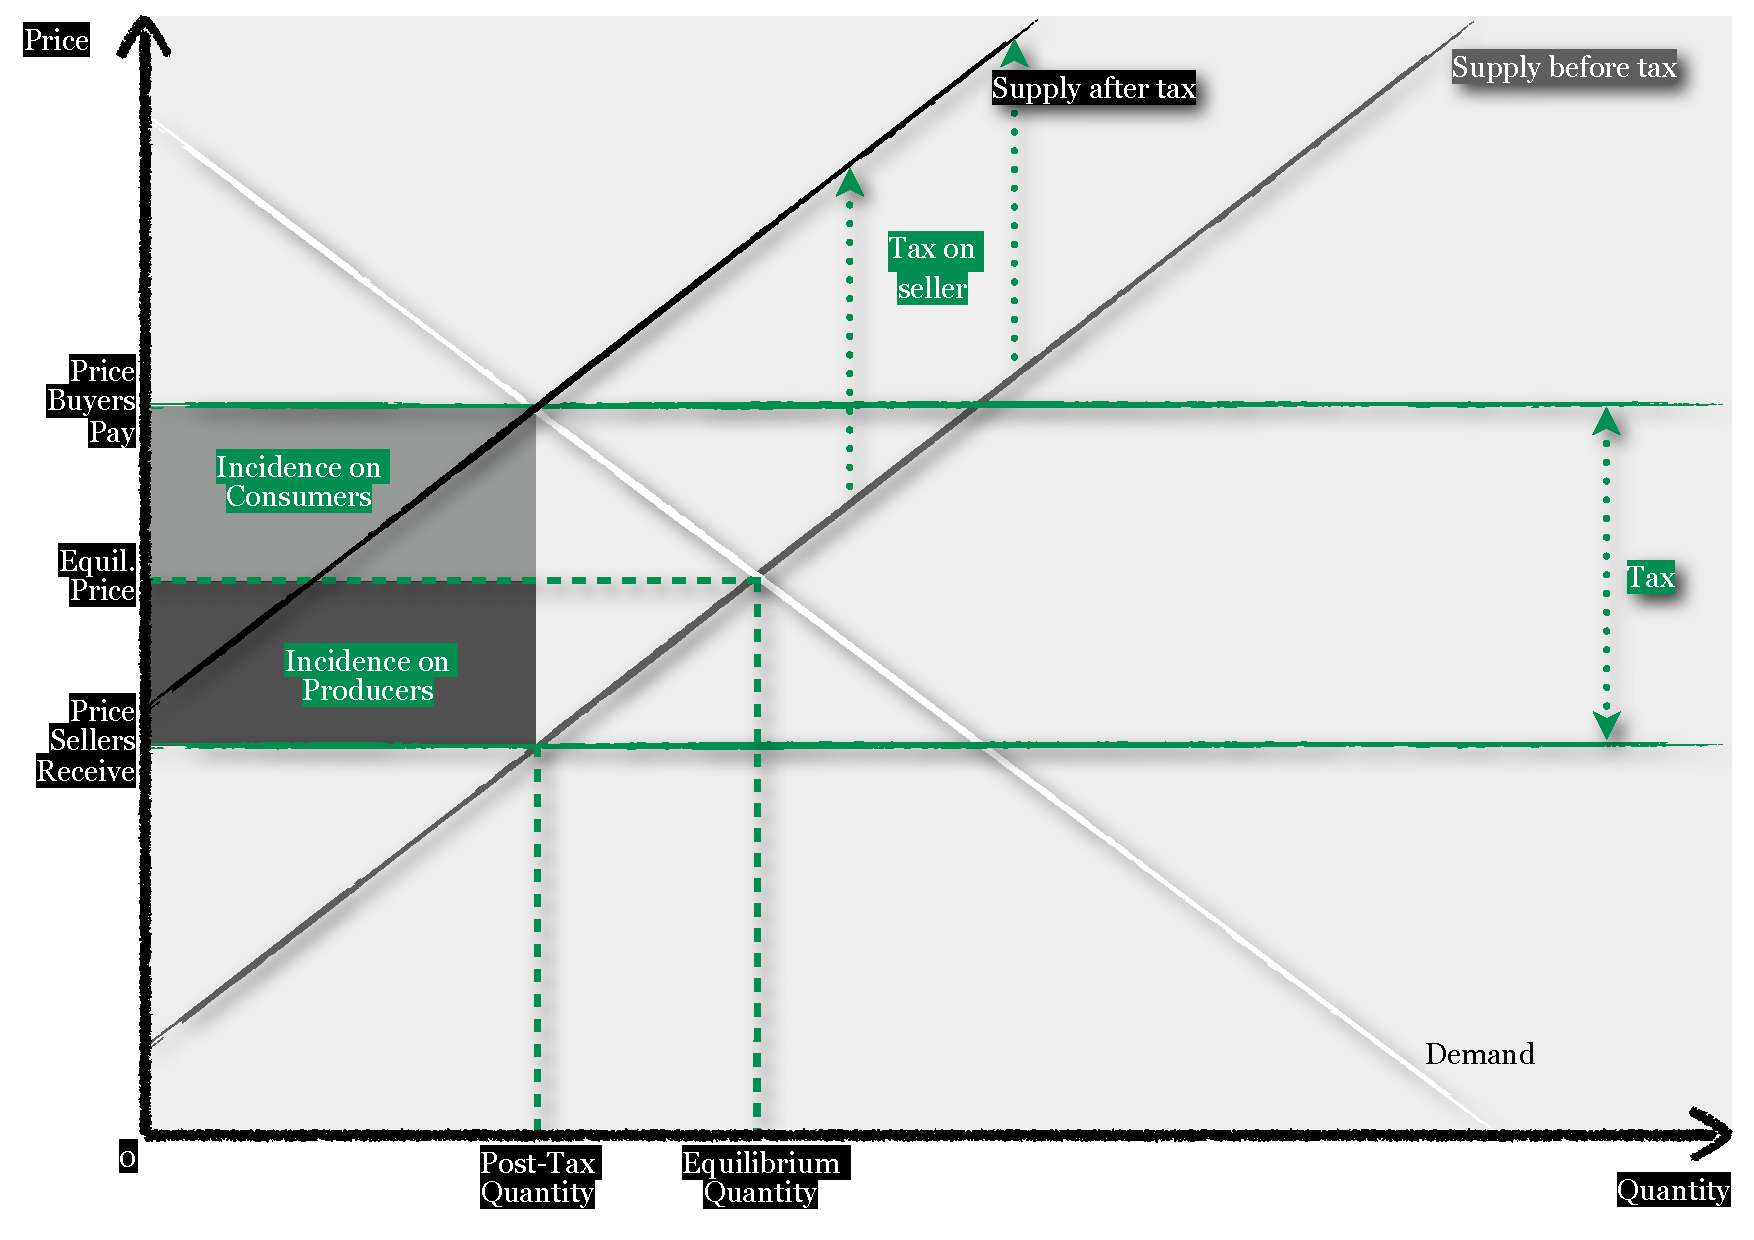
\includegraphics[width=1\textwidth]{./img/same-incidence}  
	\caption[Incidence of a Tax on Suppliers with Unit-Elastic Supply and Demand]{The Incidence of a Tax on Suppliers with Same Elasticities for Producers and Consumers}
	\label{fig:same-incidence}
\end{figure}

Taxation is always an \hyperref[sec:marketvscommand]{intervention in a market activity} (p. \pageref{sec:marketvscommand}). The incidence of a tax is borne by all parties to these market exchanges in proportion to their relative price elasticities of demand and supply, respectively, as shown in figure \ref{fig:different-incidence} (p. \pageref{fig:different-incidence}). Whoever can cheaply exit or substitute the taxed market exchange dodges most of the tax: because these price elastic suppliers \emph{would} quickly cut their quantity supplied at lower prices, they can extract relatively high prices from buyers. Buyers, in this example, cannot cheaply exit or substitute the taxed market exchange: they \emph{would} hardly be able to cut their quantity demanded in response to higher prices. At the post-tax equilibrium, buyers foot most of the tax.

 \begin{figure}[htbp]
	\centering
	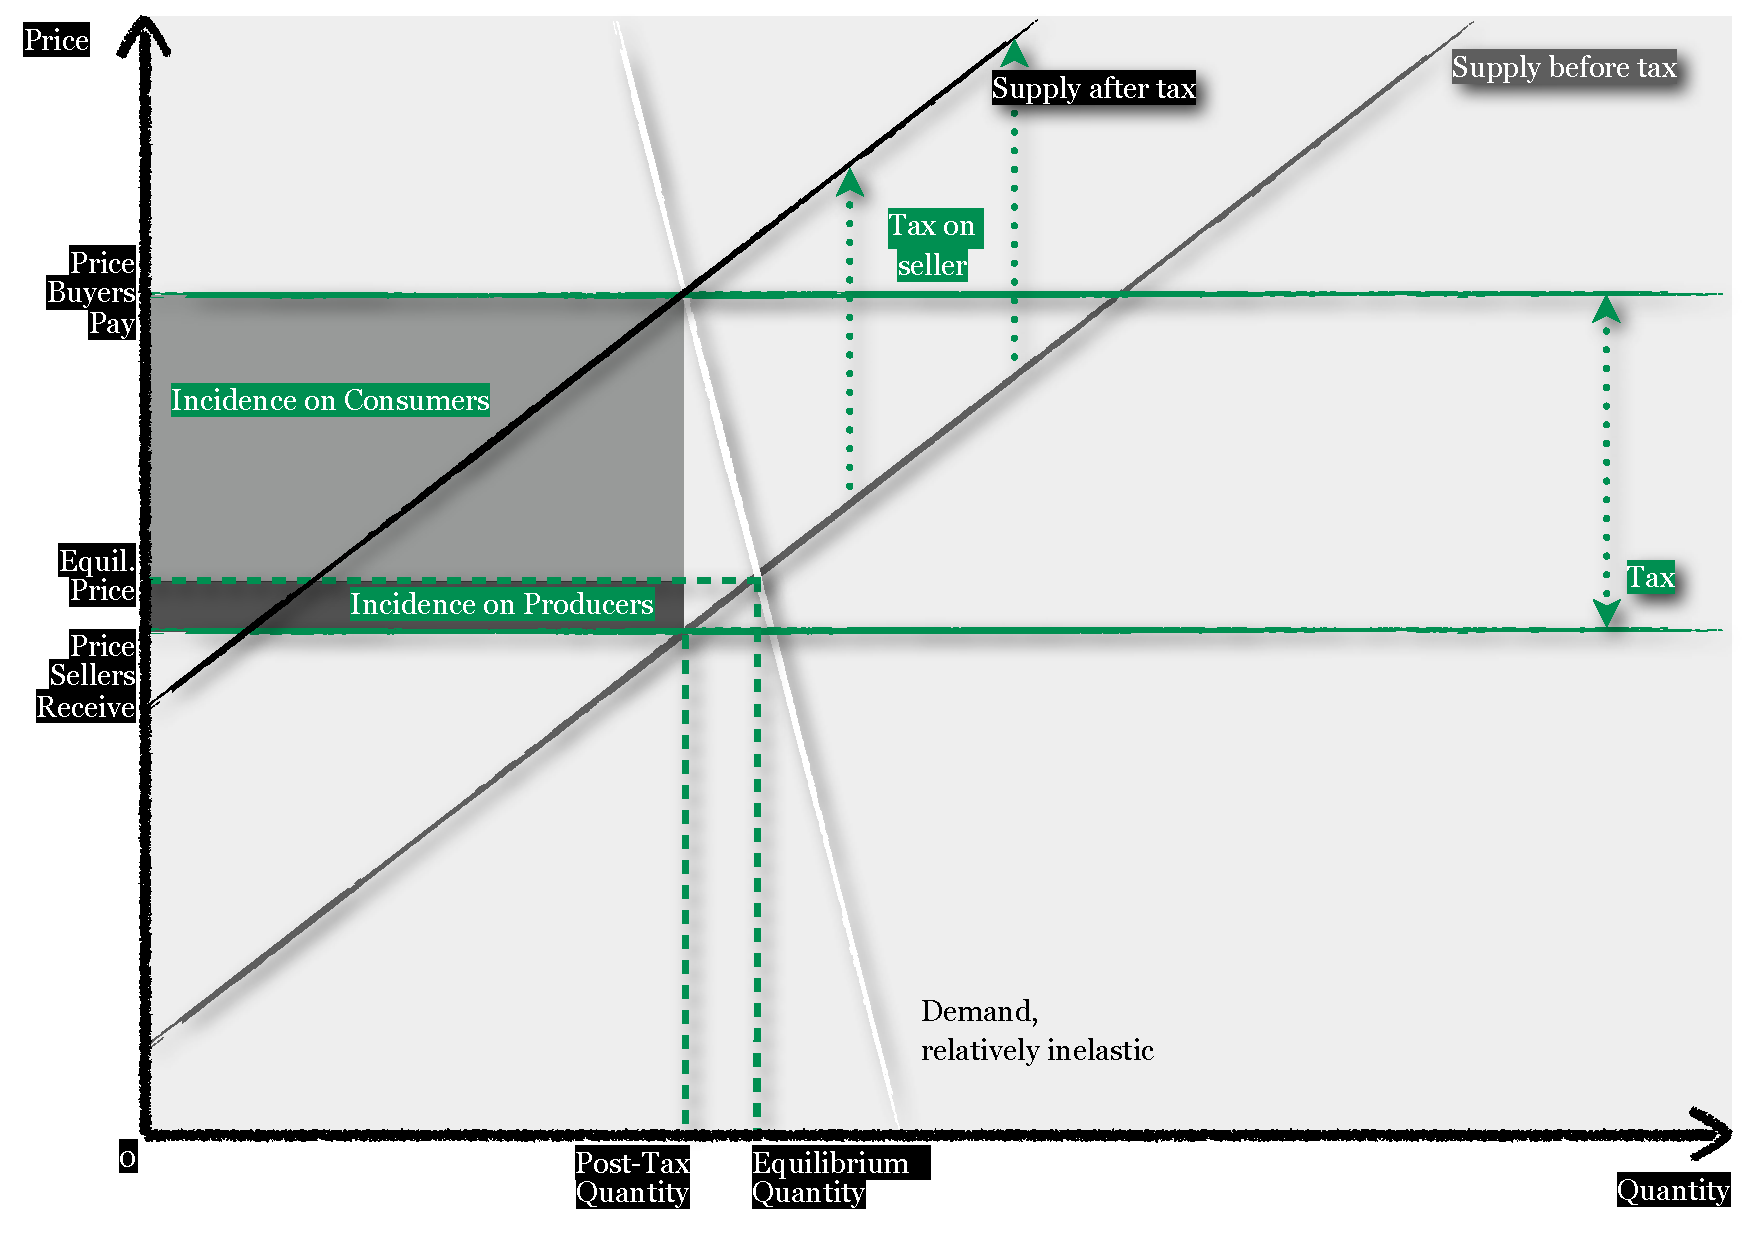
\includegraphics[width=1\textwidth]{./img/different-incidence}  
	\caption[Incidence of a Tax on Suppliers with Relatively Inelastic Demand]{The Incidence of a Tax on Suppliers with Relatively Less Elastic Demand}
	\label{fig:different-incidence}
\end{figure}

In the real world, relative price elasticities of demand and supply in many markets are unknown and would be difficult to ascertain\footnote{
	It is usually assumed that incidence applies only to \emph{indirect} taxes such as \gls{VAT} and \gls{CIT}. I find this limited application of incidence implausible. The concept remains applicable for \emph{direct} taxes, including \gls{PIT} and \gls{WT}, too. 
	
	A \gls{PIT} on labor incomes, for instance, may partially fall on employers when labor markets are very tight: tax-depressed worker supply may cause employers to pay more. Even a \gls{WT} may fall on people other than the owners when demand for their collateral is sufficiently inelastic: interest rates may rise when private capital becomes less abundant.}. 
Elasticity of demand and supply depends on many factors, including the availability of substitutes (e.g., margarine for butter) as well as the mobility and specificity of factors (e.g. immobile, specific typewriter factory vs mobile, unspecific car rental).

Therefore, to fairly and effectively redistribute between natural persons, government must tax market interactions where the relative price elasticities of demand and supply can be easily known. This is often the case for very broad categories of market exchanges, such as labor (\gls{Payroll}) or consumption (\gls{VAT})\footnote{A proportional \gls{Payroll} is actually equivalent to a \gls{VAT} in its incidence. A \gls{Payroll} taxes (only) labor income before it is spent (prepaid), a \gls{VAT} taxes (only) labor income after it is spent (postpaid).}: people cannot substitute working \emph{somewhere} or employing \emph{someone}, they cannot avoid to buying or selling \emph{something}\footnote{
	Saving is a third alternative if you subscribe to a \emph{\gls{Y2C}}: when you consider returns on capital a genuine \emph{change} in welfare, you can substitute present spending for \emph{more} future spending. 
	
	If, instead, you believe in a \emph{\gls{OSN}}, returns on capital are just compensation to risk, uncertainty and delayed pleasure: welfare is \emph{postponed}, but not changed. Consequently, under a \gls{OSN}, you can only substitute current consumption for same future consumption, and have no alternative but to spend your money at some point. 
	
	For a summary of the savings norm debate see \cite{Held2010a} or, in the brilliant original, \citeauthor{McCaffery2005} (\citeyear{McCaffery2005}: 819).}. 
The price elasticities for demand and supply in these broadly defined markets are small and similar.

In the closed economy, government can effectively tax broad categories of market exchanges, such as consumption\footnote{
	I use consumption and, broadly equivalently, labor as examples here because unlike income taxation (\gls{PIT}), they do not require me to decide on a savings norm (\gls{Y2C} or \gls{OSN}). Both norms are unattractive in the extremes and only a \gls{PCT} can resolve the tension (\citealt{Held2010a}).
	
	Still, it is important to point out that, no matter the savings norm, savers in a closed economy have limited or no alternative to investing at home. Therefore, the incidence of a \gls{PIT} will also be relatively well-defined in a closed economy.}. 
By definition, economic activity does not extent beyond the borders of the closed economy, and there can therefore be no substitution to, for example, spending at home.

\subparagraph[Tax Efficiency]{Minimal Market Distortions, Welfare Losses.} \phantomsection \label{sec:minimalDWL}
When government taxes a market exchange, buyers and sellers may react in ways that reduce overall welfare. 

When the post-tax price of the transaction is higher than the buyers utility or the sellers cost, they exit the market. Their otherwise pareto-improving exchange does not occur, as shown in figure \ref{fig:DWL} (p. \pageref{fig:DWL}). Government also gains no revenue from these non-occurring transactions. Everybody loses. The sum total of these losses is known as the \gls{DWL} of taxation (areas C, E in figure \href{fig:DWL}). An efficient tax minimizes \gls{DWL} for maximum revenue (areas B, D).

\begin{figure}[htbp]
	\centering
	\includegraphics[width=1\textwidth]{./img/DWL}  
	\caption[Deadweight-Loss of a Tax with Unit-Elastic Supply and Demand]{The \gls{DWL} of a Tax with Unit-Elastic Supply and Demand}
	\label{fig:DWL}
\end{figure}

This ratio of tax revenue to \gls{DWL} --- much like the \hyperref[sec:well-determinedincidence]{effective incidence of a tax} (p. \pageref{sec:well-determinedincidence}) --- depends on the price elasticities of supply and demand. The more inelastic supply and demand, the smaller the \gls{DWL} for any given tax rate, as shown in figure \ref{fig:smaller-DWL} (p. \pageref{fig:smaller-DWL}). If buyers and sellers cannot easily cease their welfare-improving exchanges, they will continue to trade when taxed. A tax on such a market will not distort or depress market activities.

\begin{figure}[htbp]
	\centering
	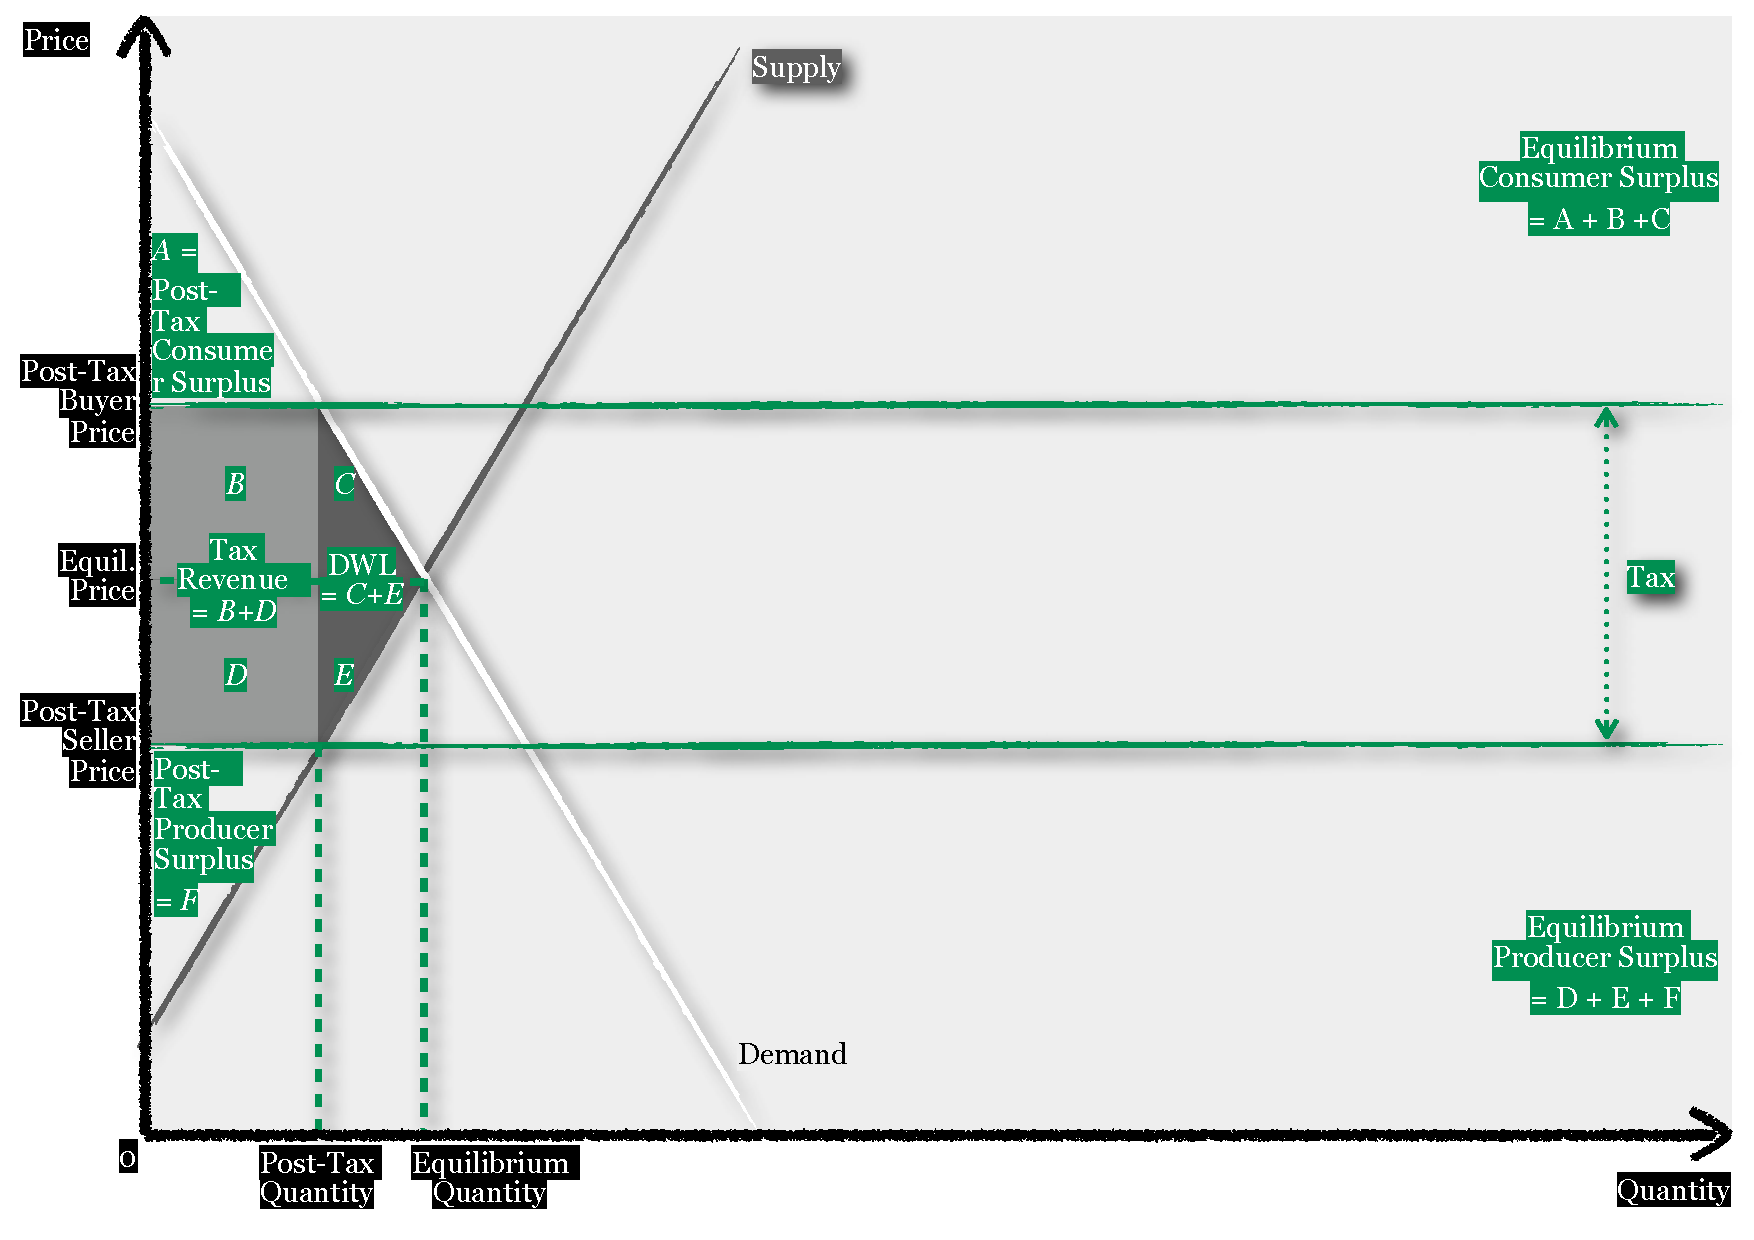
\includegraphics[width=1\textwidth]{./img/smaller-DWL}  
	\caption[Deadweight-Loss of a Tax with Inelastic Suppy and Demand]{The Deadweight-Loss of a Tax with Inelastic Supply and Demand}
	\label{fig:smaller-DWL}
\end{figure}

The price elasticities of demand and supply are, again, a hard, empirical question. As discussed above, supply and demand in broad categories of market exchanges, such as all domestic consumption (\gls{VAT}) or all domestic labor (\gls{Payroll}) are relatively inelastic, and the \gls{DWL} of such taxes is likely to be small in a closed economy.

Still, \glspl{DWL} of taxation may abound, even in closed economies. In mixed economies, the market for low-wage labor is particularly vulnerable to large \gls{DWL}s. Welfare state governments  \hyperref[sec:distribution]{may find it necessary to give handouts} to people who earn too little to maintain a socially acceptable standard of living (p. \pageref{sec:distribution}). 

In this scenario, taxation of low-wage labor has two related, negative effects\footnote{
	As explained in the above, both a \gls{Payroll} and a \gls{VAT} burden low-wage labor.}. 
\begin{enumerate}
	\item Taxation raises the effective cost of living for low-wage earners: for each euro they earn on the market, they can afford a lower, real standard of living. 
	\item If people can apply for handouts, their supply of labor may become perfectly price elastic, when market incomes are close to welfare incomes. If they could earn less on the market, than by collecting welfare, low-wage workers may be forced to exit the labor market: a large \gls{DWL} ensues\footnote{
		In this extreme case, the \gls{DWL} of a welfare handout is equivalent to the \gls{DWL} of a price floor on labor at the same level.}. 
	Any tax on low-wage labor will only increase the \gls{DWL}: for every euro of wages taxed, more people will be pushed outside the (official) labor market\footnote{
		People leaving the labor market in this scenario has nothing to do with laziness. The legislated minimum standard of living is after all considered minimally acceptable. People who opt for welfare instead of poorly paid work may not have a choice.}. 
\end{enumerate}

In the closed economy, government can minimize the tax burden on low-wage labor by relying more on progressive taxes, including a \gls{PIT}, instead of proportional taxes (\gls{VAT}, \gls{Payroll}).


\subsubsection[Monetary Policy]{The Means of Monetary Policy} \label{sec:monetary}
Government provides the economy with legal tender to serve as \begin{inparaenum}[1)] 
	\item a medium of exchange, 
	\item a unit of account and 
	\item a store of value. 
\end{inparaenum} 
Only government can do this, because supplying money is a \hyperref[sec:naturalmonopoly]{natural monopoly} (p. \pageref{sec:naturalmonopoly}). To avoid the \hyperref[sec:pricestability]{costs} (p. \pageref{sec:pricestability}) and  \hyperref[sec:distributive-effects-of-inflation]{arbitrary redistribution} (p. \pageref{sec:distributive-effects-of-inflation}) of de- or inflation, 
governments should be devoted to price stability. 

They set that quantity of money where it equilibrates with variable money \emph{demand} at stable prices. The demand for money, in turn, is determined by the output of the economy\footnote{
	This very brief account follows the \emph{quantity} theory of money. Competing theories are discussed in the below.}.

\paragraph[Tools]{Tools.} Government extends or contracts the supply of money to meet a quantity, interest rate (US) or inflation rate (Bundesbank) target. Fiat money\footnote{
	If for no other reason, fiat money would be preferable to intrinsically valuable moneys \emph{because} governments can adjust its supply to output in the long run and at little cost. By contrast, specie moneys are costly to extract and their supply changes arbitarily on new discovery. 
	
	The futility of a gold-based economy is aptly summarized by investor Warren Buffett: ``[Gold] gets dug out of the ground in Africa, or someplace. Then we melt it down, dig another hole, bury it again and pay people to stand around guarding it. (...) Anyone watching from Mars would be scratching their head.''} 
is supplied in two ways:
\begin{enumerate}
	\item Government creates \emph{base money} by \begin{inparaenum}[a)] 
		\item buying government bonds (\gls{OMO}) or 
		\item other financial assets (\gls{QE}) from private holders who receive legal tender out of thin air\footnote{
			Actually, the balance sheet of the central bank records the acquired bond as an asset, and the currency as a liability.} 
		in return
			\footnote{Central banks are customarily barred from buying government bonds directly from government to increase transparency. By buying government bonds from a middlewoman, central banks can still ``print money''.}.
		Central banks can also 
		\item lend money to financial institutions at a set rate (discount window rate).
	\end{inparaenum}
	\item Government stimulates the multiplication of \emph{broad money} in the fractional reserve banking system by lowering the reserve requirements for private banks.
\end{enumerate}

 \begin{figure}[htbp]
	\centering
	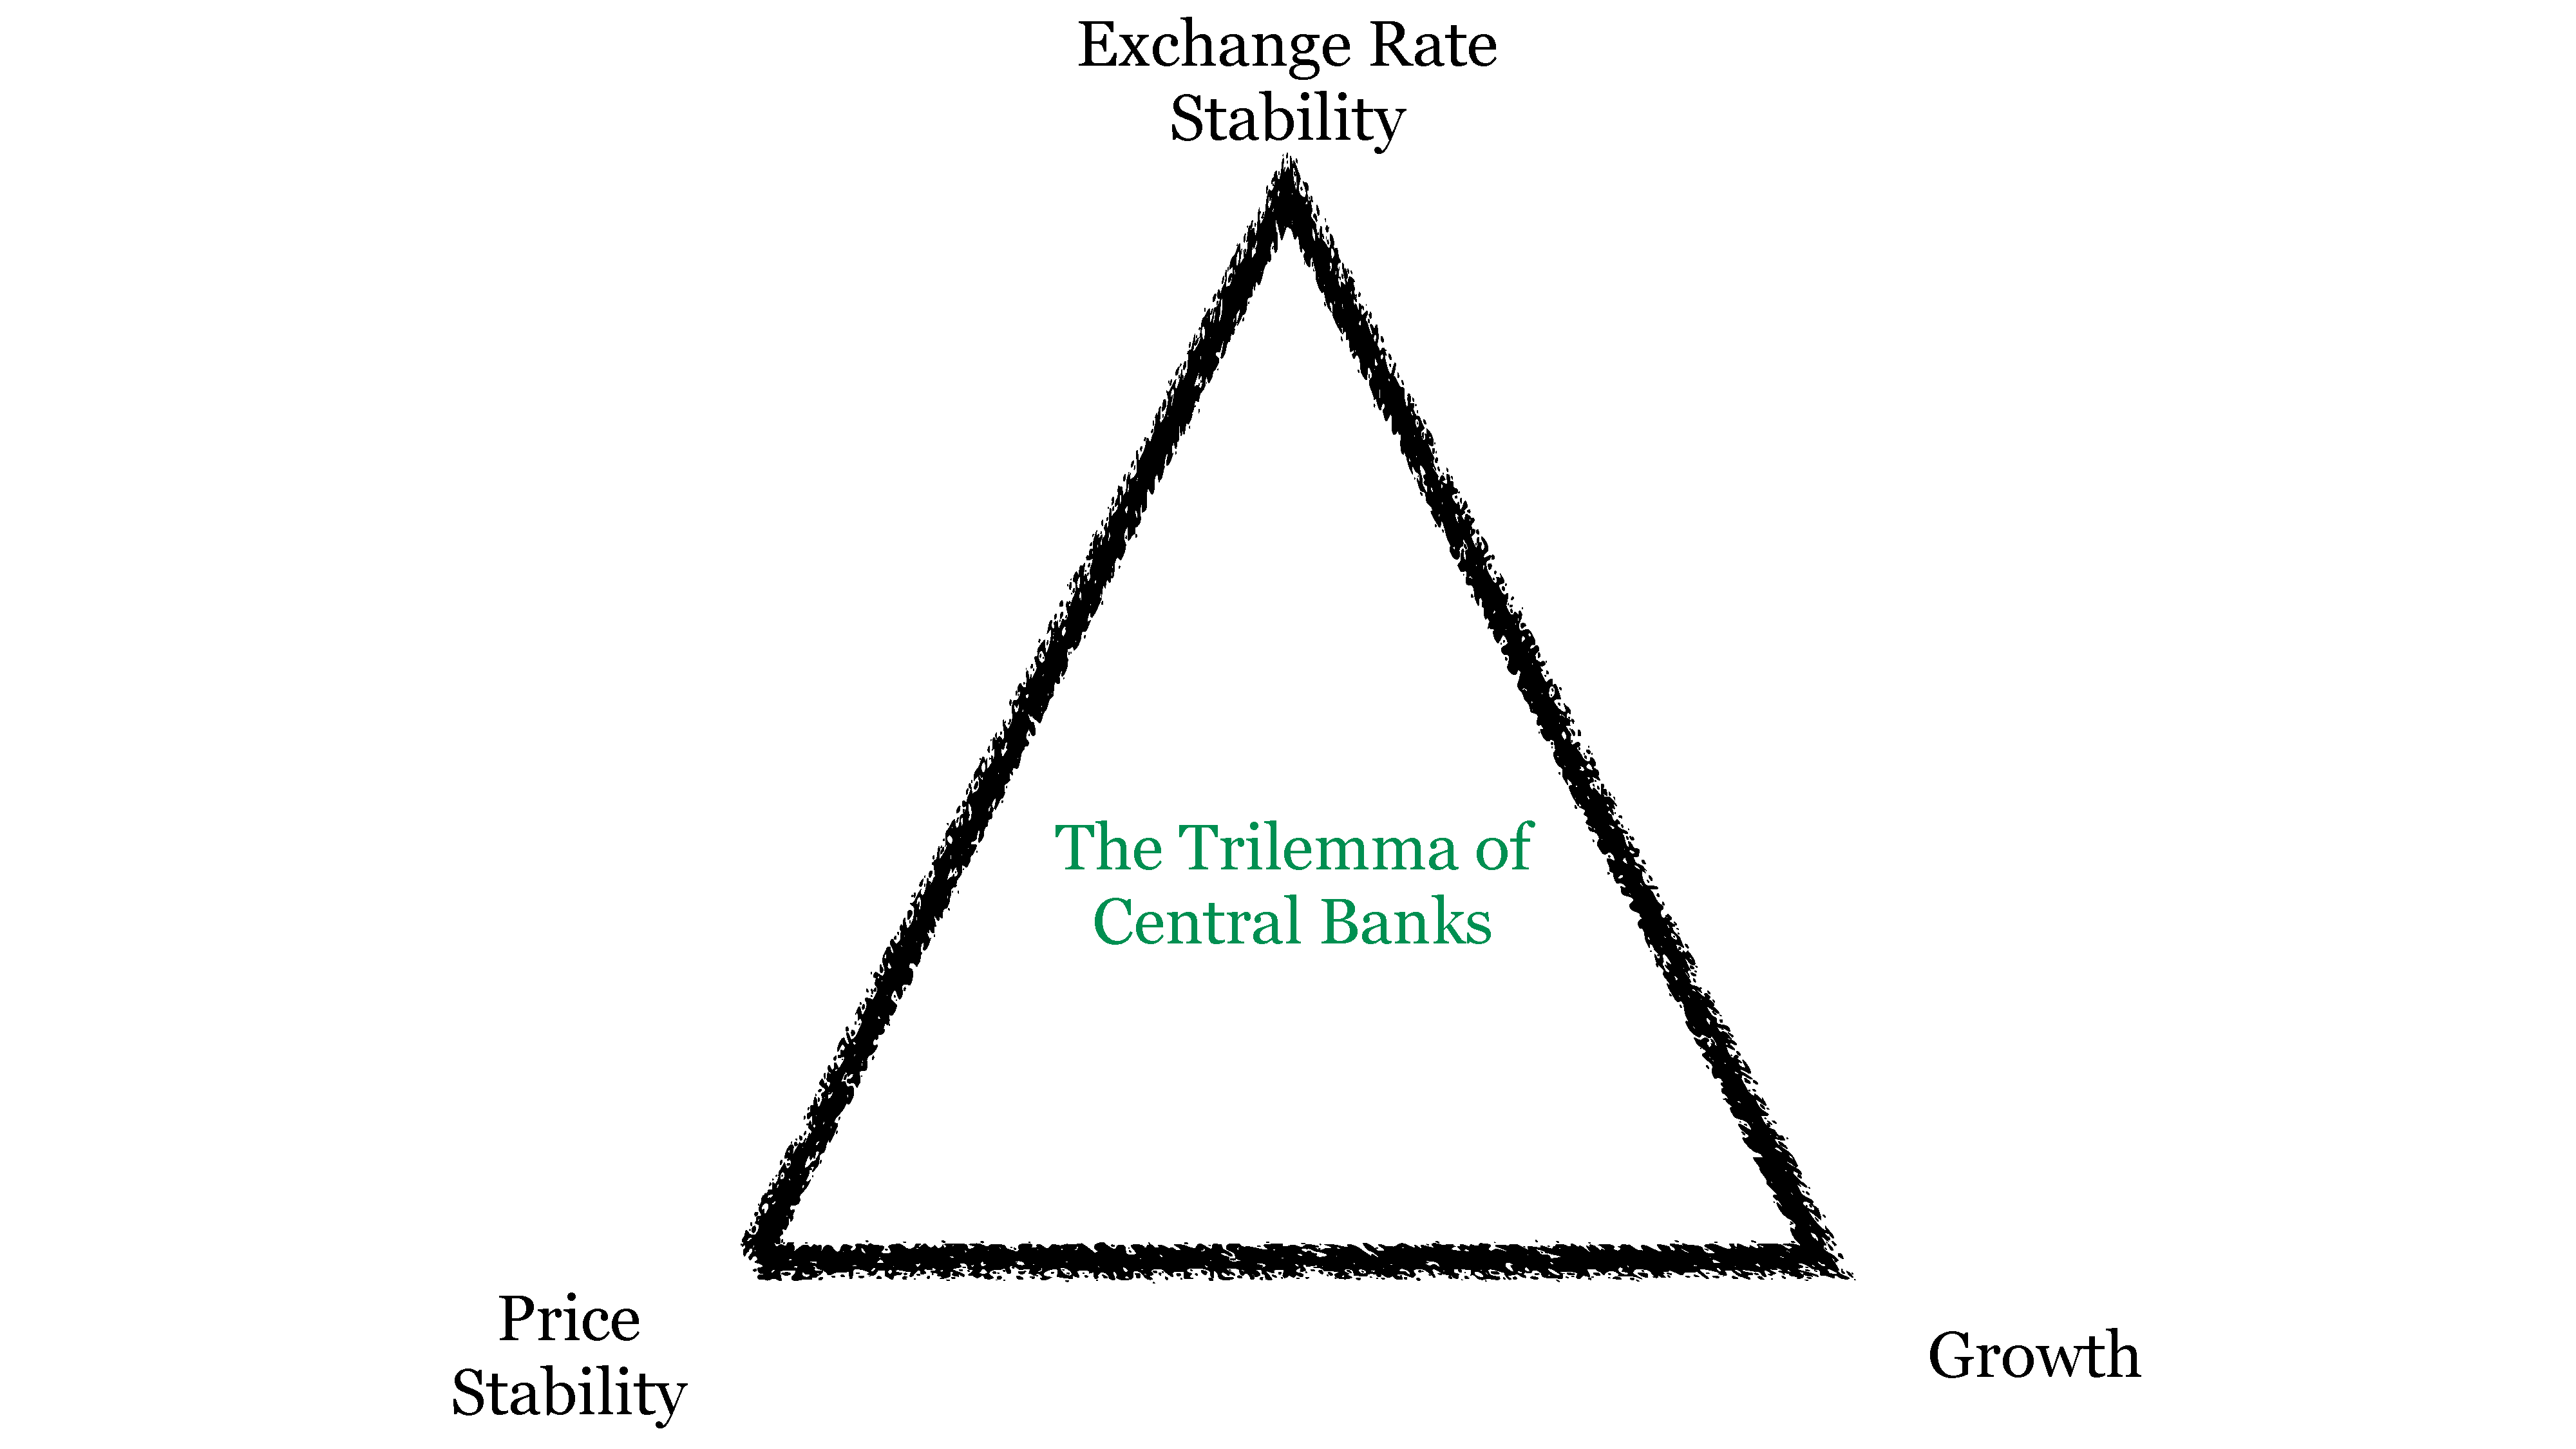
\includegraphics[width=1\linewidth]{./img/triangle-cb}  
	\caption{The Policy Trilemma of Central Banks}
	\label{fig:triangle-cb}
\end{figure}

\paragraph[Role]{Role.} %This section is horseshit.
The impact of monetary policy on the real economy is, of course, incompletely understood and highly controversial. I do not need to recapitulate these controversies here (for a recent review, see \citealt{Wapshott2011}). I note two hopefully uncontroversial points:

\begin{enumerate}
	\item \emph{Monetary Neutrality.} \label{it:monetaryneutrality} Following the classical dichotomy, \emph{nominal} economic variables, such as the price level, do not matter in the long run. The prosperity of an economy is determined by its level of technology, human capital and physical capital --- not by the amount of intrinsically worthless currency in circulation. 
	
	On this ultimate end of monetary policy, Monetarists and Keynesians can probably agree: good money stays out of way of the real economy to let actual output track the long-term growth path of the economy.

	\item \emph{An Empirical Question.} Different monetary theories follow from different assumptions about human behavior:

	\begin{description}
		\item[Keynesians] believe that market participants are swayed by changes in nominal variables. As a result, the prices for goods and services and factor prices (especially wages) do not equilibrate promptly or perfectly. Self-reinforcing (debt-deflation) crises of excess supply and depressed demand may result \citep{Fisher1933}. The state can smooth out resulting aggregate fluctuations in output by altering the money supply. 
		\item[Monetarists] believe that market participants are fairly rational and will consider expectations of future inflation (and taxes) in their current decisions. As a result, prices for goods and services and factor prices, especially wages, equilibrate quickly and keep the economy on its long-term growth trajectory. State intervention in the business cycle\footnote{
			This according to \gls{RBCT}.} 
		or the money supply are unneccessary and ineffective\footnote{
			This according to the policy ineffectiveness proposition}.
	\end{description}

	Determining our irrational \emph{animal spirits} \citep{Keynes1936} is an empirical question best left to cognitive psychology, behavioral economics and related fields (recently \citealt{Akerlof2010})\footnote{
		Indeed, monetary policy seems greatly concerned with mass psychology, or \emph{open-mouth-operations} in addition to \gls{OMO}s. For example, according to rational expectations theory, it is important for a central bank to \emph{appear} credibly tough on inflation to keep inflation down.}. 
	
	``Keynes v. Hayek'' \citep{Wapshott2011} need not be a normative struggle, but a pragmatic balance based on empirical evidence. Whichever policy stabilizes economic output along the long-term growth trajectory is best. 
	
	If ever there was a policy that should be judged on consequentialist terms, it is monetary policy.
\end{enumerate}

Because monetary dynamics \emph{do not} and \emph{should not} matter to our `household with a cast of billions' I can refer the issue to empirical clarification and need not entertain it further here. Suffice it to remind us that government should set that quantity of money where it equilibrates with variable money demand at stable prices. The rest is empirical details.

\subsection[Tradeoffs]{Tradeoffs} \label{sec:tradeoffs} Given its conflicting \hyperref[sec:ends]{ends} (p. \pageref{sec:ends}) the mixed economy can arrange its \hyperref[sec:means]{means} (p. \pageref{sec:means}) to make at least two basic trade-offs. 
\begin{enumerate}
	\item \emph{Command vs. Exchange.} It can organize more or less production and distribution by command instead of exchange. 
	\item \emph{Consumption vs. Saving.} It can defer more or less of current consumption to the future. 
\end{enumerate}	
	
We can look at these tradeoffs by \hyperref[sec:byexpenditure]{expenditure} (p. \pageref{sec:byexpenditure}) and by \hyperref[sec:deltanetworth]{changes in net worth} (p. \pageref{sec:deltanetworth}) of the entire economy. 

\paragraph[By Expenditure]{By Expenditure.} \phantomsection \label{sec:byexpenditure}
A mixed economy can devote its resources (expenses) to public or private, investment and consumption goods. The four expenditure components and revenue flows are plotted on a two-dimensional coordinate space of the mixed economy in figure \ref{fig:coordinate-space} (p. \pageref{fig:coordinate-space}). I provide (very roughly) equivalent macroeconomic variables as \hyperref[tab:GDPCompExp]{components of GDP by expenditure} in table \ref{tab:GDPCompExp} (p. \pageref{tab:GDPCompExp})\footnote{
	\gls{GDP} and its macroeconomic components, while commonly reported, falls short of a comprehensive account of the economy. 
	
	Rather than a measure of prosperity, it indicates market value level of economic \emph{activity}. Roughly, \gls{GDP} is to prosperity, as a corporation's cash flow statement is to its income statement. \gls{GDP} growth and positive cash flows are a necessary, but not a sufficient condition to prosperity. 
	
	\gls{GDP} does not measure changes in net worth as an income statement would: for example, an earthquake (or nuclear power disaster, or both) can raise \gls{GDP} because of reconstruction \emph{activities}, even if it actually wiped out \emph{assets}. \gls{GDP} also excludes environmental degredation or use of natural resources.
	
	Lastly, \gls{GDP} falls short, because it records only activity with a market value; economic activity in the household or family are not included, as are social costs or utility of market activities (externalities).}.
	
\begin{landscape}
 \begin{figure}[htbp]
	\centering
	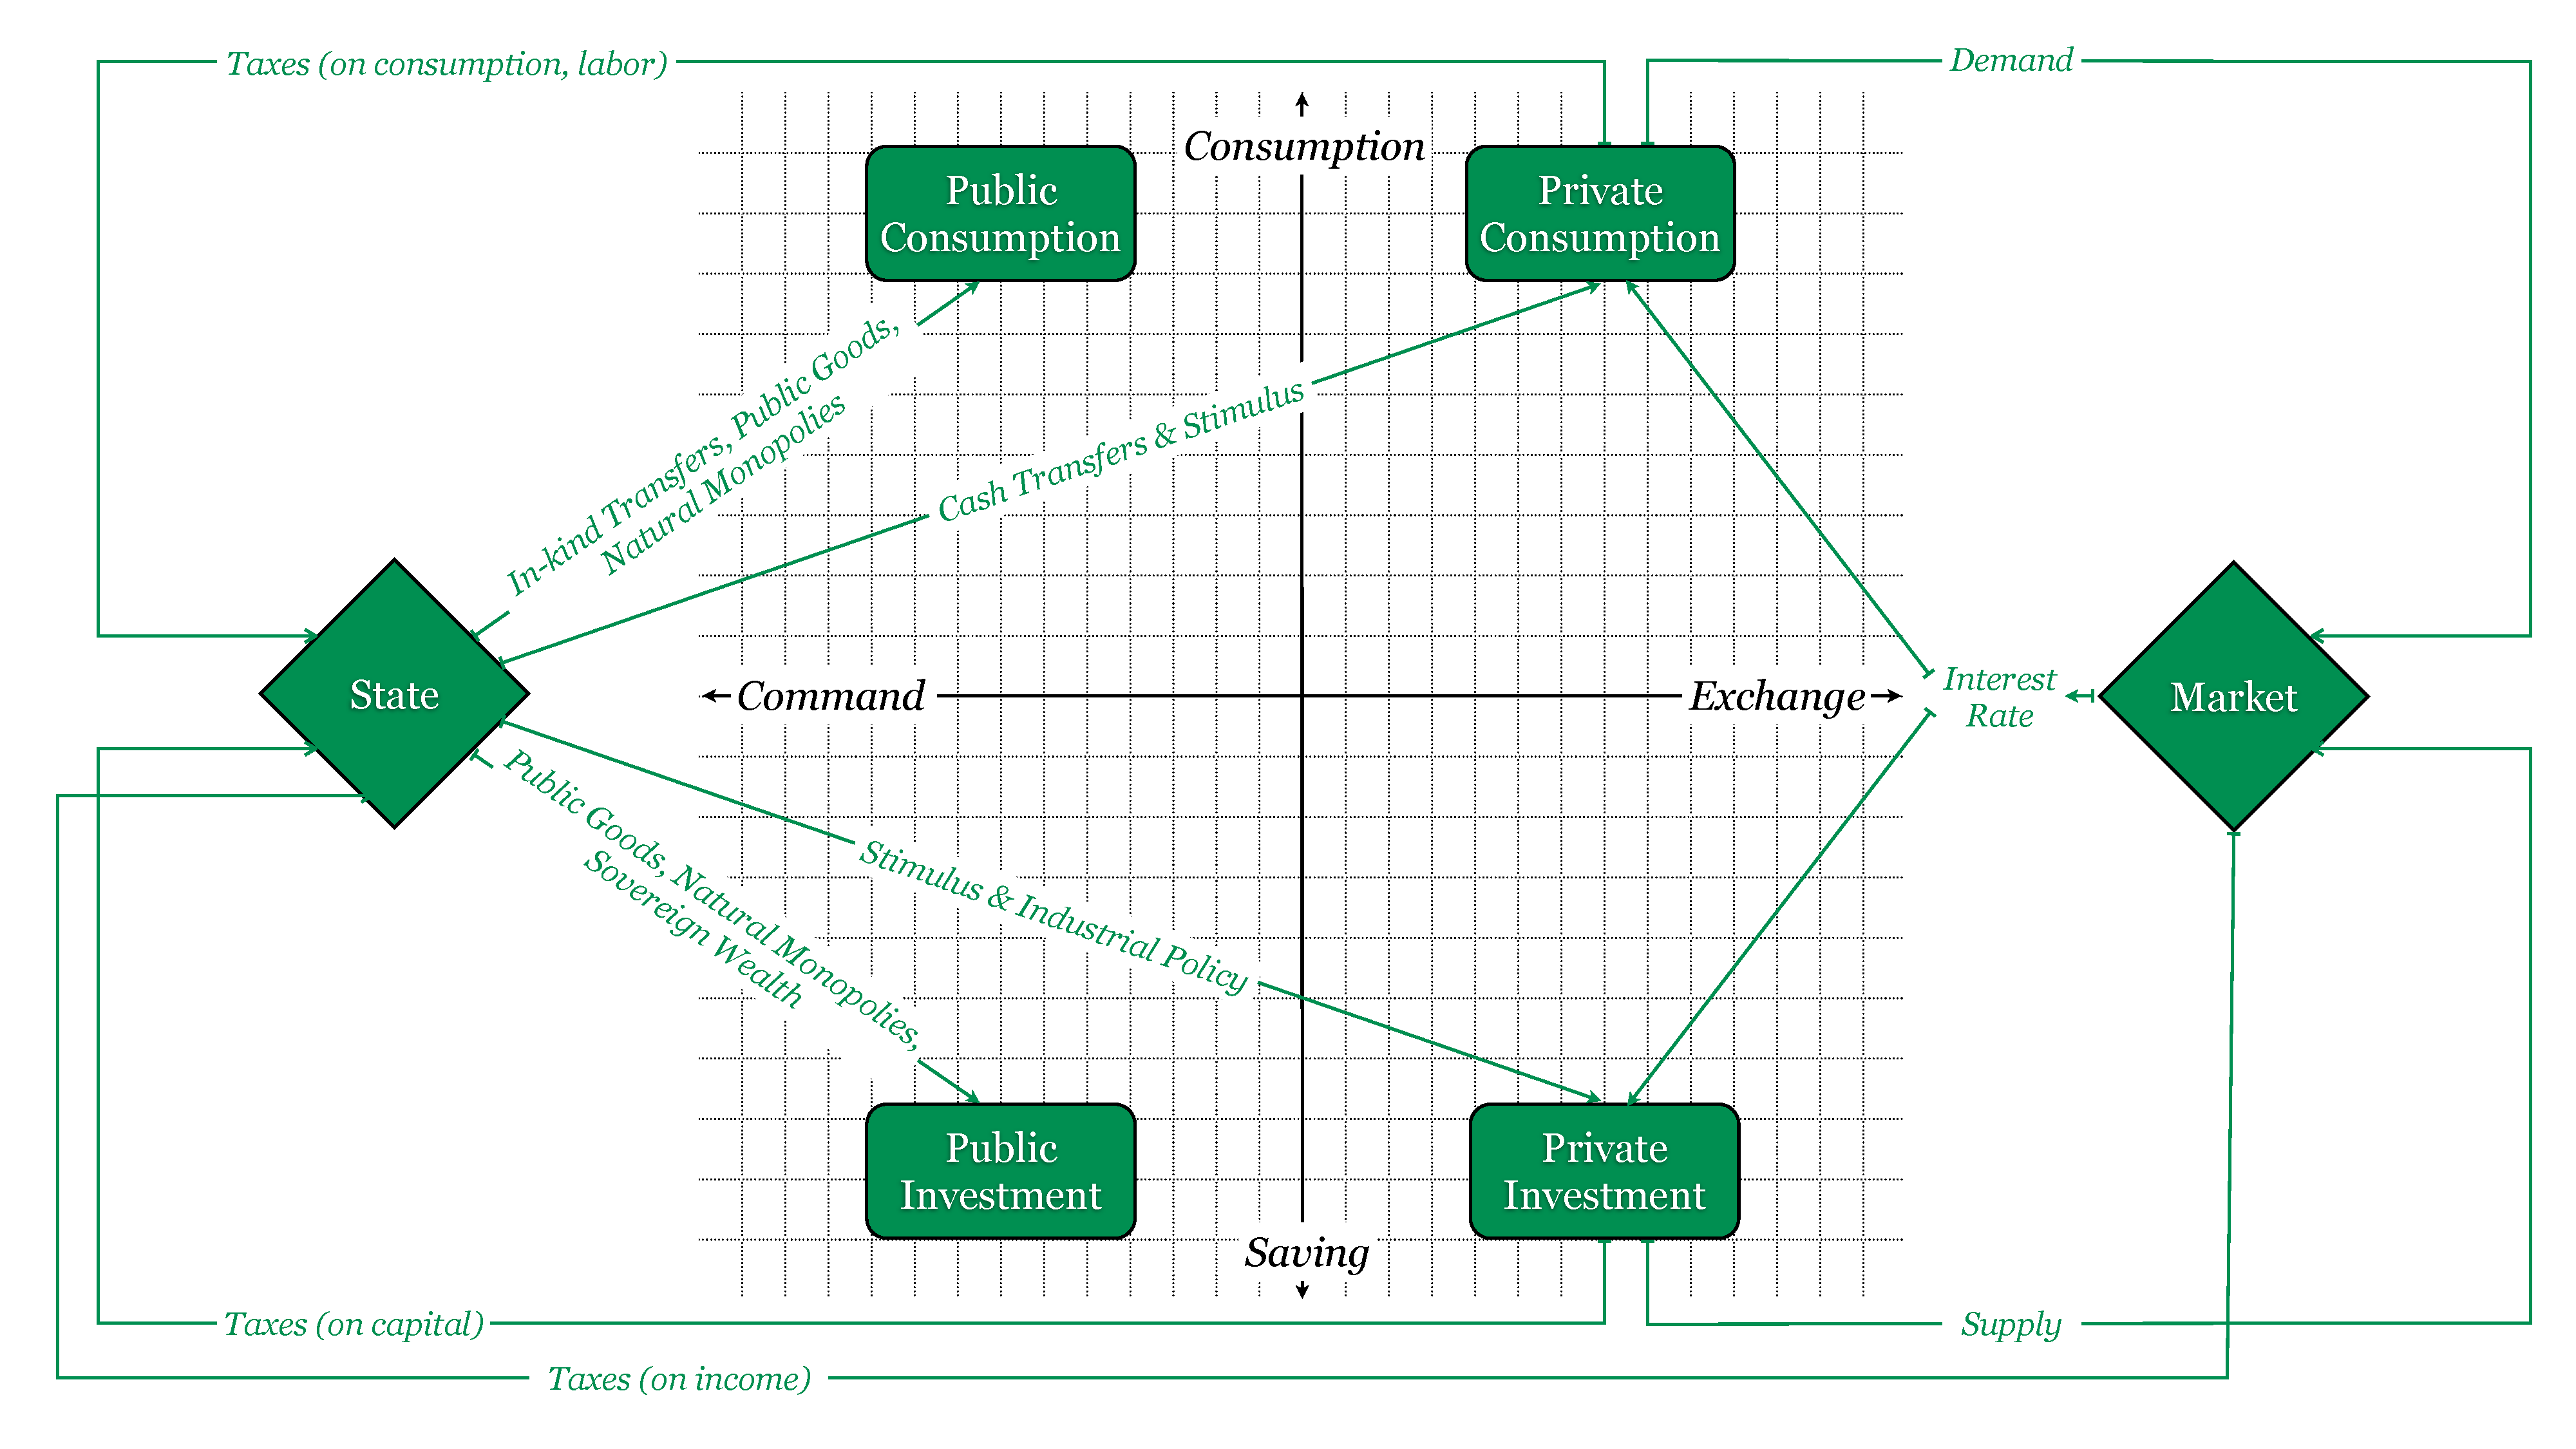
\includegraphics[width=1\linewidth]{./img/coordinate-space}  
	\caption{Coordinate Space of the Mixed Economy}
	\label{fig:coordinate-space}
\end{figure} %add squalor etc. to the coordinate space 
\end{landscape}

\begin{figure}[htbp]
	\centering
	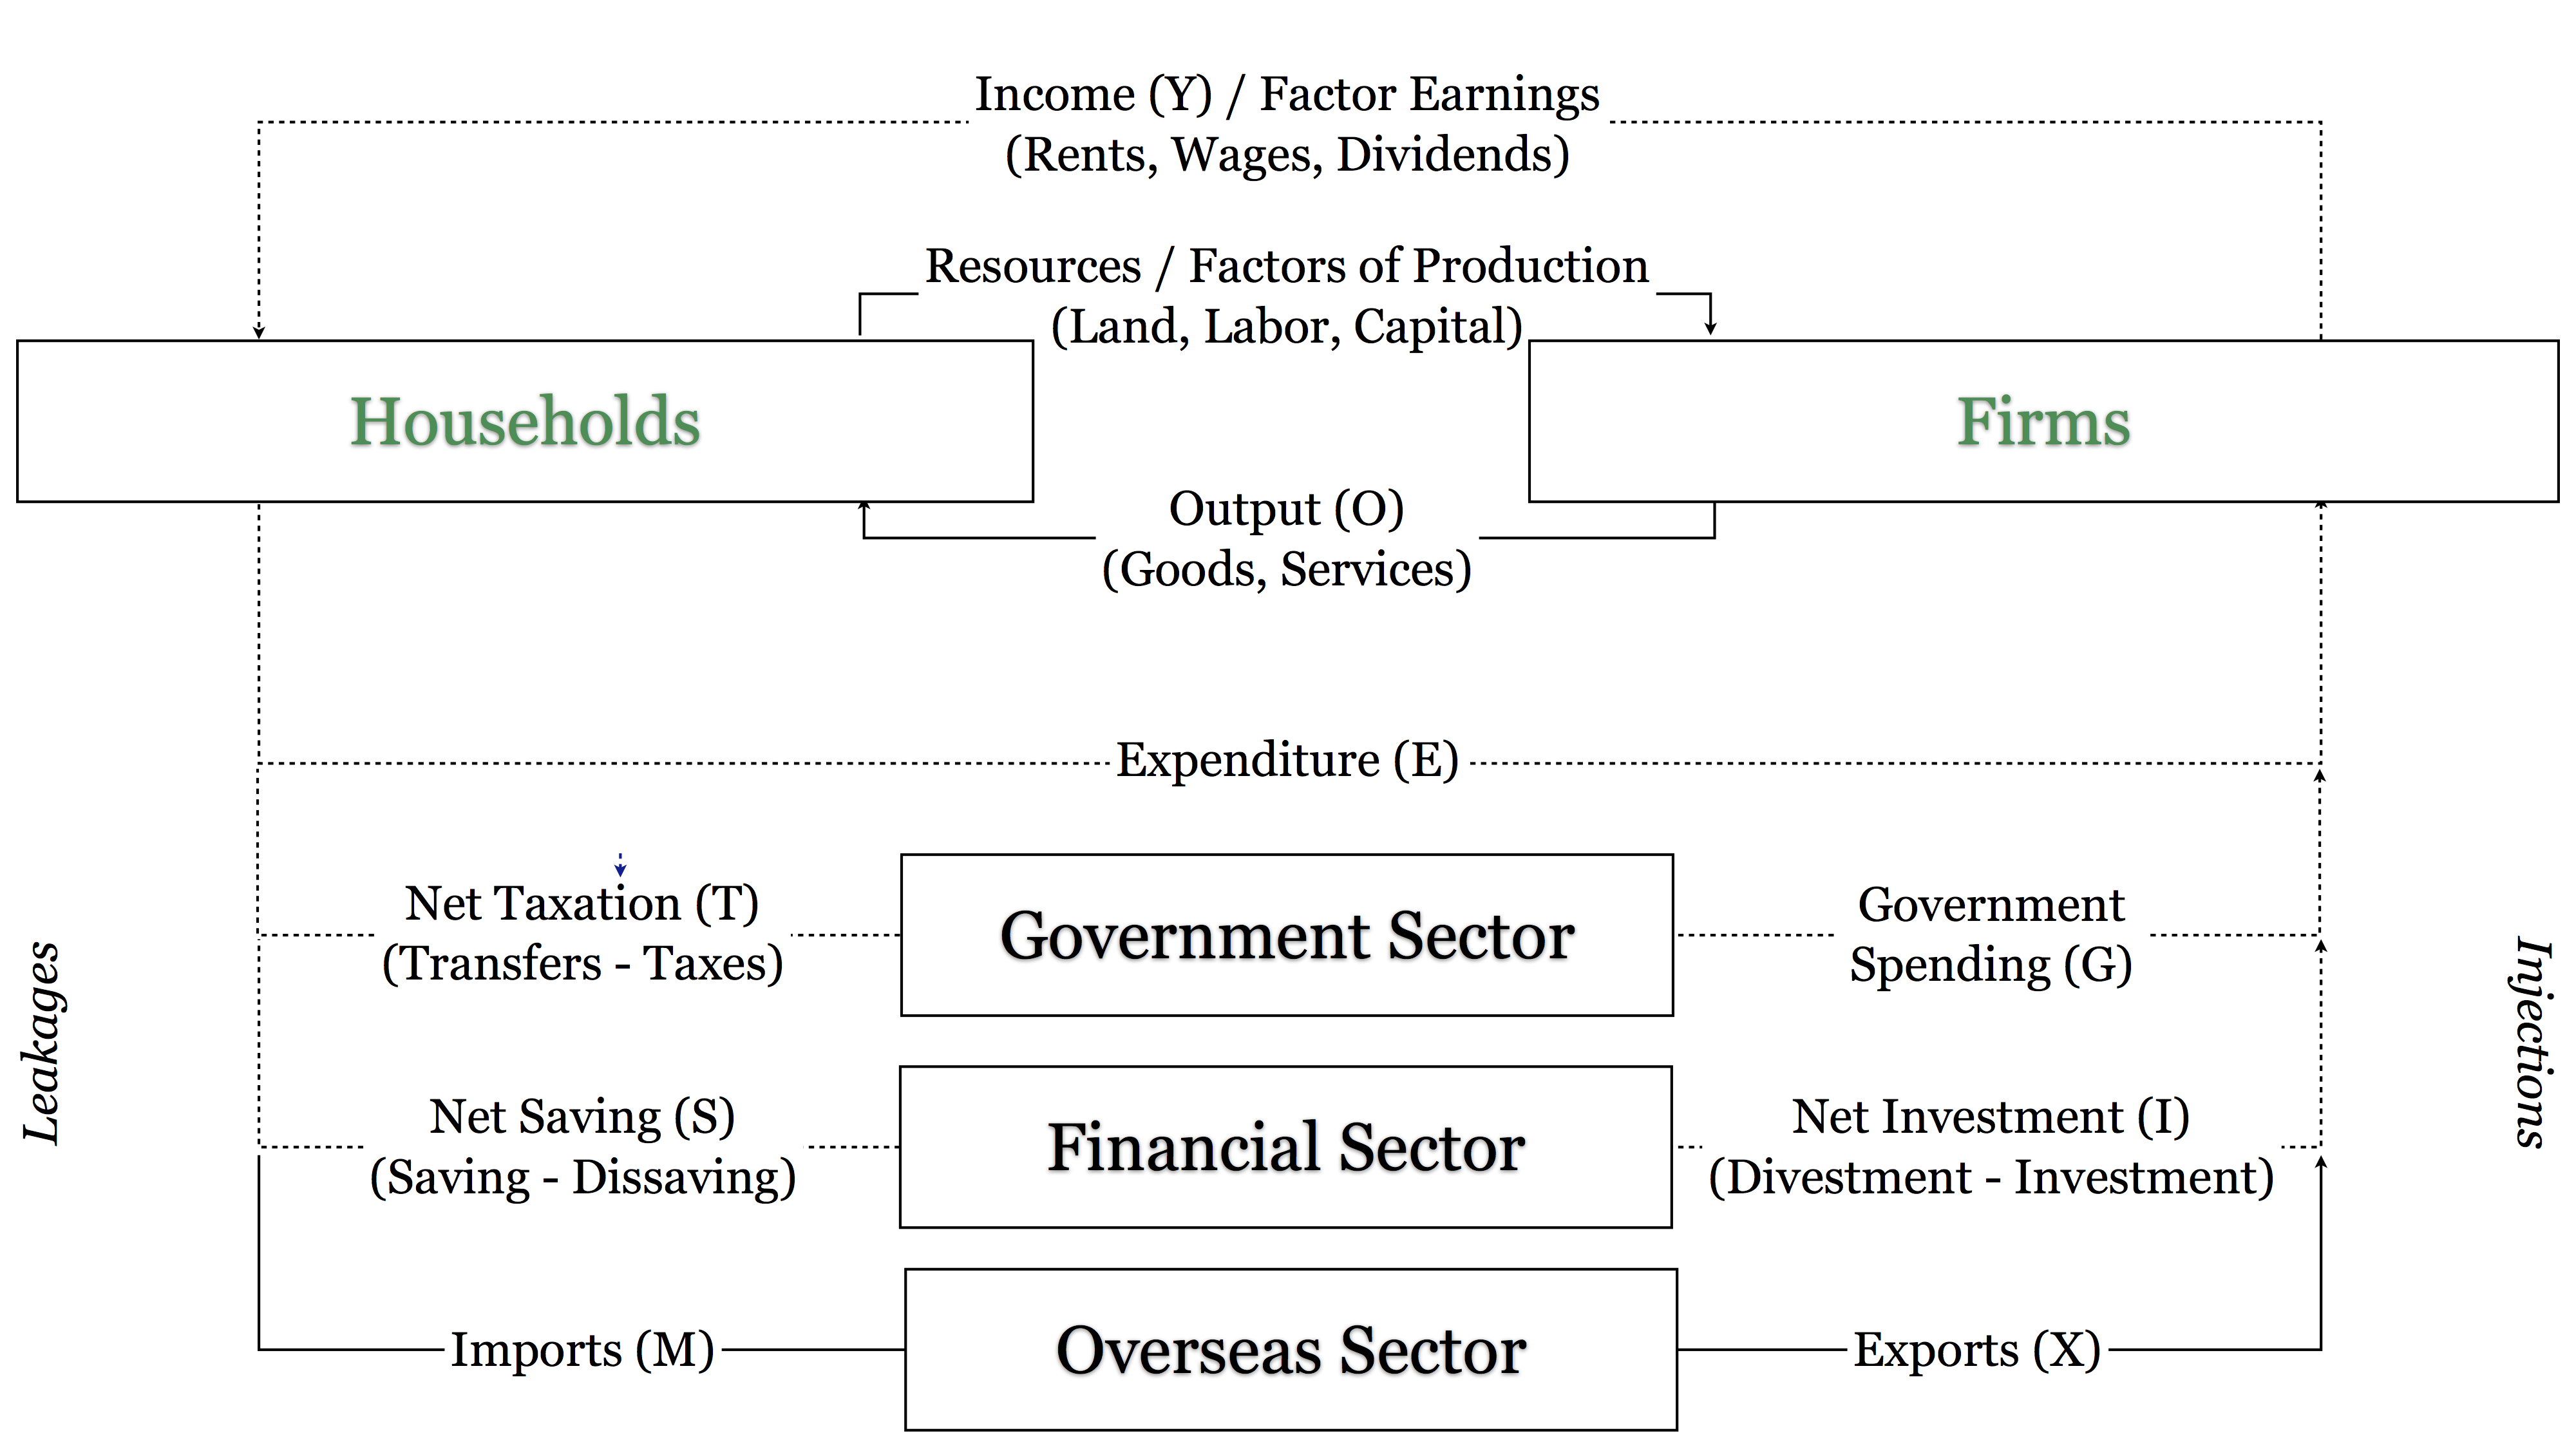
\includegraphics[width=1\textwidth]{./img/circular-flow}  
	\caption[Circular Flow in the Economy]{Circular Flow of Income in the Economy}
	\begin{flushleft}
		\scriptsize{via \href{http://en.wikipedia.org/wiki/circular-flowofincome}{Wikipedia}}.
	\end{flushleft}
	\label{fig:circular-flow}
\end{figure}

%add somewhere a section on why saving doesn't lead to low demand. BASTARD KEYNESIANISM. Gotcha.
\subparagraph[Save More or Less]{Save/Consume More or Less.} Government increases the private savings rate by taxing consumption (instead of income), encouraging investment (factory) through industrial policy or other fiscal stimulus and increases public saving by putting net tax revenue into durable public goods (basic research), natural monopolies (a bridge) or \glsplural{SWF}. 

Steering in the opposite direction, government increases private consumption by cash transfers, fiscal stimulus and public consumption by handing out in-kind benefits (school milk), or providing short-term public goods (fireworks) and natural monopolies. The saving-consumption tradeoff roughly expressed in the gross savings rate in table \ref{tab:GDPCompExp} (p. \pageref{tab:GDPCompExp}) \footnote{
	GDP-related metrics fall short, again: \gls{GFCF} and consequently the gross savings rate does not include capital depreciation. It also does not include real dissavings on goods without a market value, such as the population growth rate or environmental quality. 
	
	Consequently, gross savings rates may be overstated in existing accounts.}.

	% why aren't public budgets documented like the budgets of private firms, including a full balance sheet? how is this ENRON accounting even possible?

\subparagraph[Exchange-Command Mix]{More or Less Government/Market} Government sets the exchange-command mix of the economy by taxing more or less of economic output, and commissioning public investment and consumption from the revenue. The exchange-command mix is (roughly) expressed in the public expenditure quota in table \ref{tab:GDPCompExp} (p. \pageref{tab:GDPCompExp}).

\subparagraph[Optima]{How to Strike the Best Balance.} Welfare economics and the \hyperref[sec:ends]{ends} of a mixed economy (p. \pageref{sec:ends}) suggests that there are one (or more) \emph{optima} in the balance between saving and consumption, between market and command. These ends also bind each of the government interventions, such as providing a public good, to \emph{specific} justifications\footnote{
	Justifying a choice of the mixed economy does not mean that it can be reduced to a positive question. Ends and means such as redistribution may, and maybe should, remain contested.}, 
such as a market failure in providing the public good. Normatively, government \emph{should} not take an arbitrary position on \hyperref[fig:coordinate-space]{the coordinate space of the mixed economy} (figure \ref{fig:coordinate-space}). 

However, I should point out that \emph{positively}, government in a closed economy \emph{could} employ its \hyperref[sec:means]{means} to choose any of the possible tradeoffs between consumption and saving, market and command economy. 
	%does this table actually correspond to all the state jobs, or just some?

\subparagraph[Tax is Key]{Tax is Key.} Of these \hyperref[sec:means]{means} of the mixed economy, tax is the dominant tool. To redirect resources between the four quadrants, government relies primarily on \hyperref[sec:fiscal]{taxation} (p. \pageref{sec:fiscal}) rather than on \hyperref[sec:regulatory]{regulation} (p. \pageref{sec:regulatory}) which has limited applications and \hyperref[sec:monetary]{money} (p. \pageref{sec:monetary}) which is neutral in the long run.

\begin{landscape}%check this table again, very thorougly.
\begin{table}
	\caption{GDP Components by Expenditure in the Closed Economy}
	\label{tab:GDPCompExp}
	\small
	\begin{center}
	\renewcommand{\arraystretch}{1.5}
	\begin{tabular}{llccrr}
		\toprule
		& & \multicolumn{2}{c}{\emph{Ownership}} & &\\
		\cmidrule(r){3-4}
		& &\emph{Private} & \emph{Public}& &\\
		\midrule
		\multirow{2}{*}{\emph{}} & \emph{\gls{I}} & Factory,  \gls{RnD} & Bridge, basic research & \emph{$\sum=$\gls{GFCF}} & \multirow{2}{*}{\emph{$\frac{\gls{GFCF}}{\gls{GDP}}=$Gross Savings Rate}}\\
		& \emph{\gls{C}} & TV set, vacation & School milk, fireworks & \emph{$\sum=$\gls{FCE}}  \\
		\midrule
		& &\emph{$\sum=$($\gls{I}+\gls{C}$)} & \emph{$\sum=$\gls{G}\footnote{\Gls{GDP} also does not, as implied in figure \ref{fig:coordinate-space} distinguish between public consumption and public investment, but lumps both together in \gls{G}.}}\\
		\cmidrule(r){3-4}
		& & \multicolumn{2}{c}{$\frac{\gls{G}}{\gls{GDP}}=$ Public expenditure quota} \\
		\bottomrule
	\end{tabular}
	\end{center}
\end{table}
\end{landscape}

\paragraph{By Changes in Net Worth} \phantomsection \label{sec:deltanetworth} The same tradeoffs of the mixed economy can also be understood as different changes in net worth. 

As economies, firms and households save and consume, their net worth changes. This truism is expressed in the Haig-Simons income identity:

\begin{equation} \label{eq:haig-simons}
			\text{Income}=\text{Consumption}+\Delta\text{Wealth}
\end{equation}

Or, trivially transformed:
\begin{equation} \label{eq:haig-simonstradeoff}
			\text{Savings}-\text{Dissavings}=\text{Income}-\text{Consumption}
\end{equation}

Figure \ref{fig:haig-simons-individual-collective} applies equation \ref{eq:haig-simonstradeoff} to the savings tradeoff of households, firms and government, including some examples. 

\begin{figure}[htbp]
	\centering
	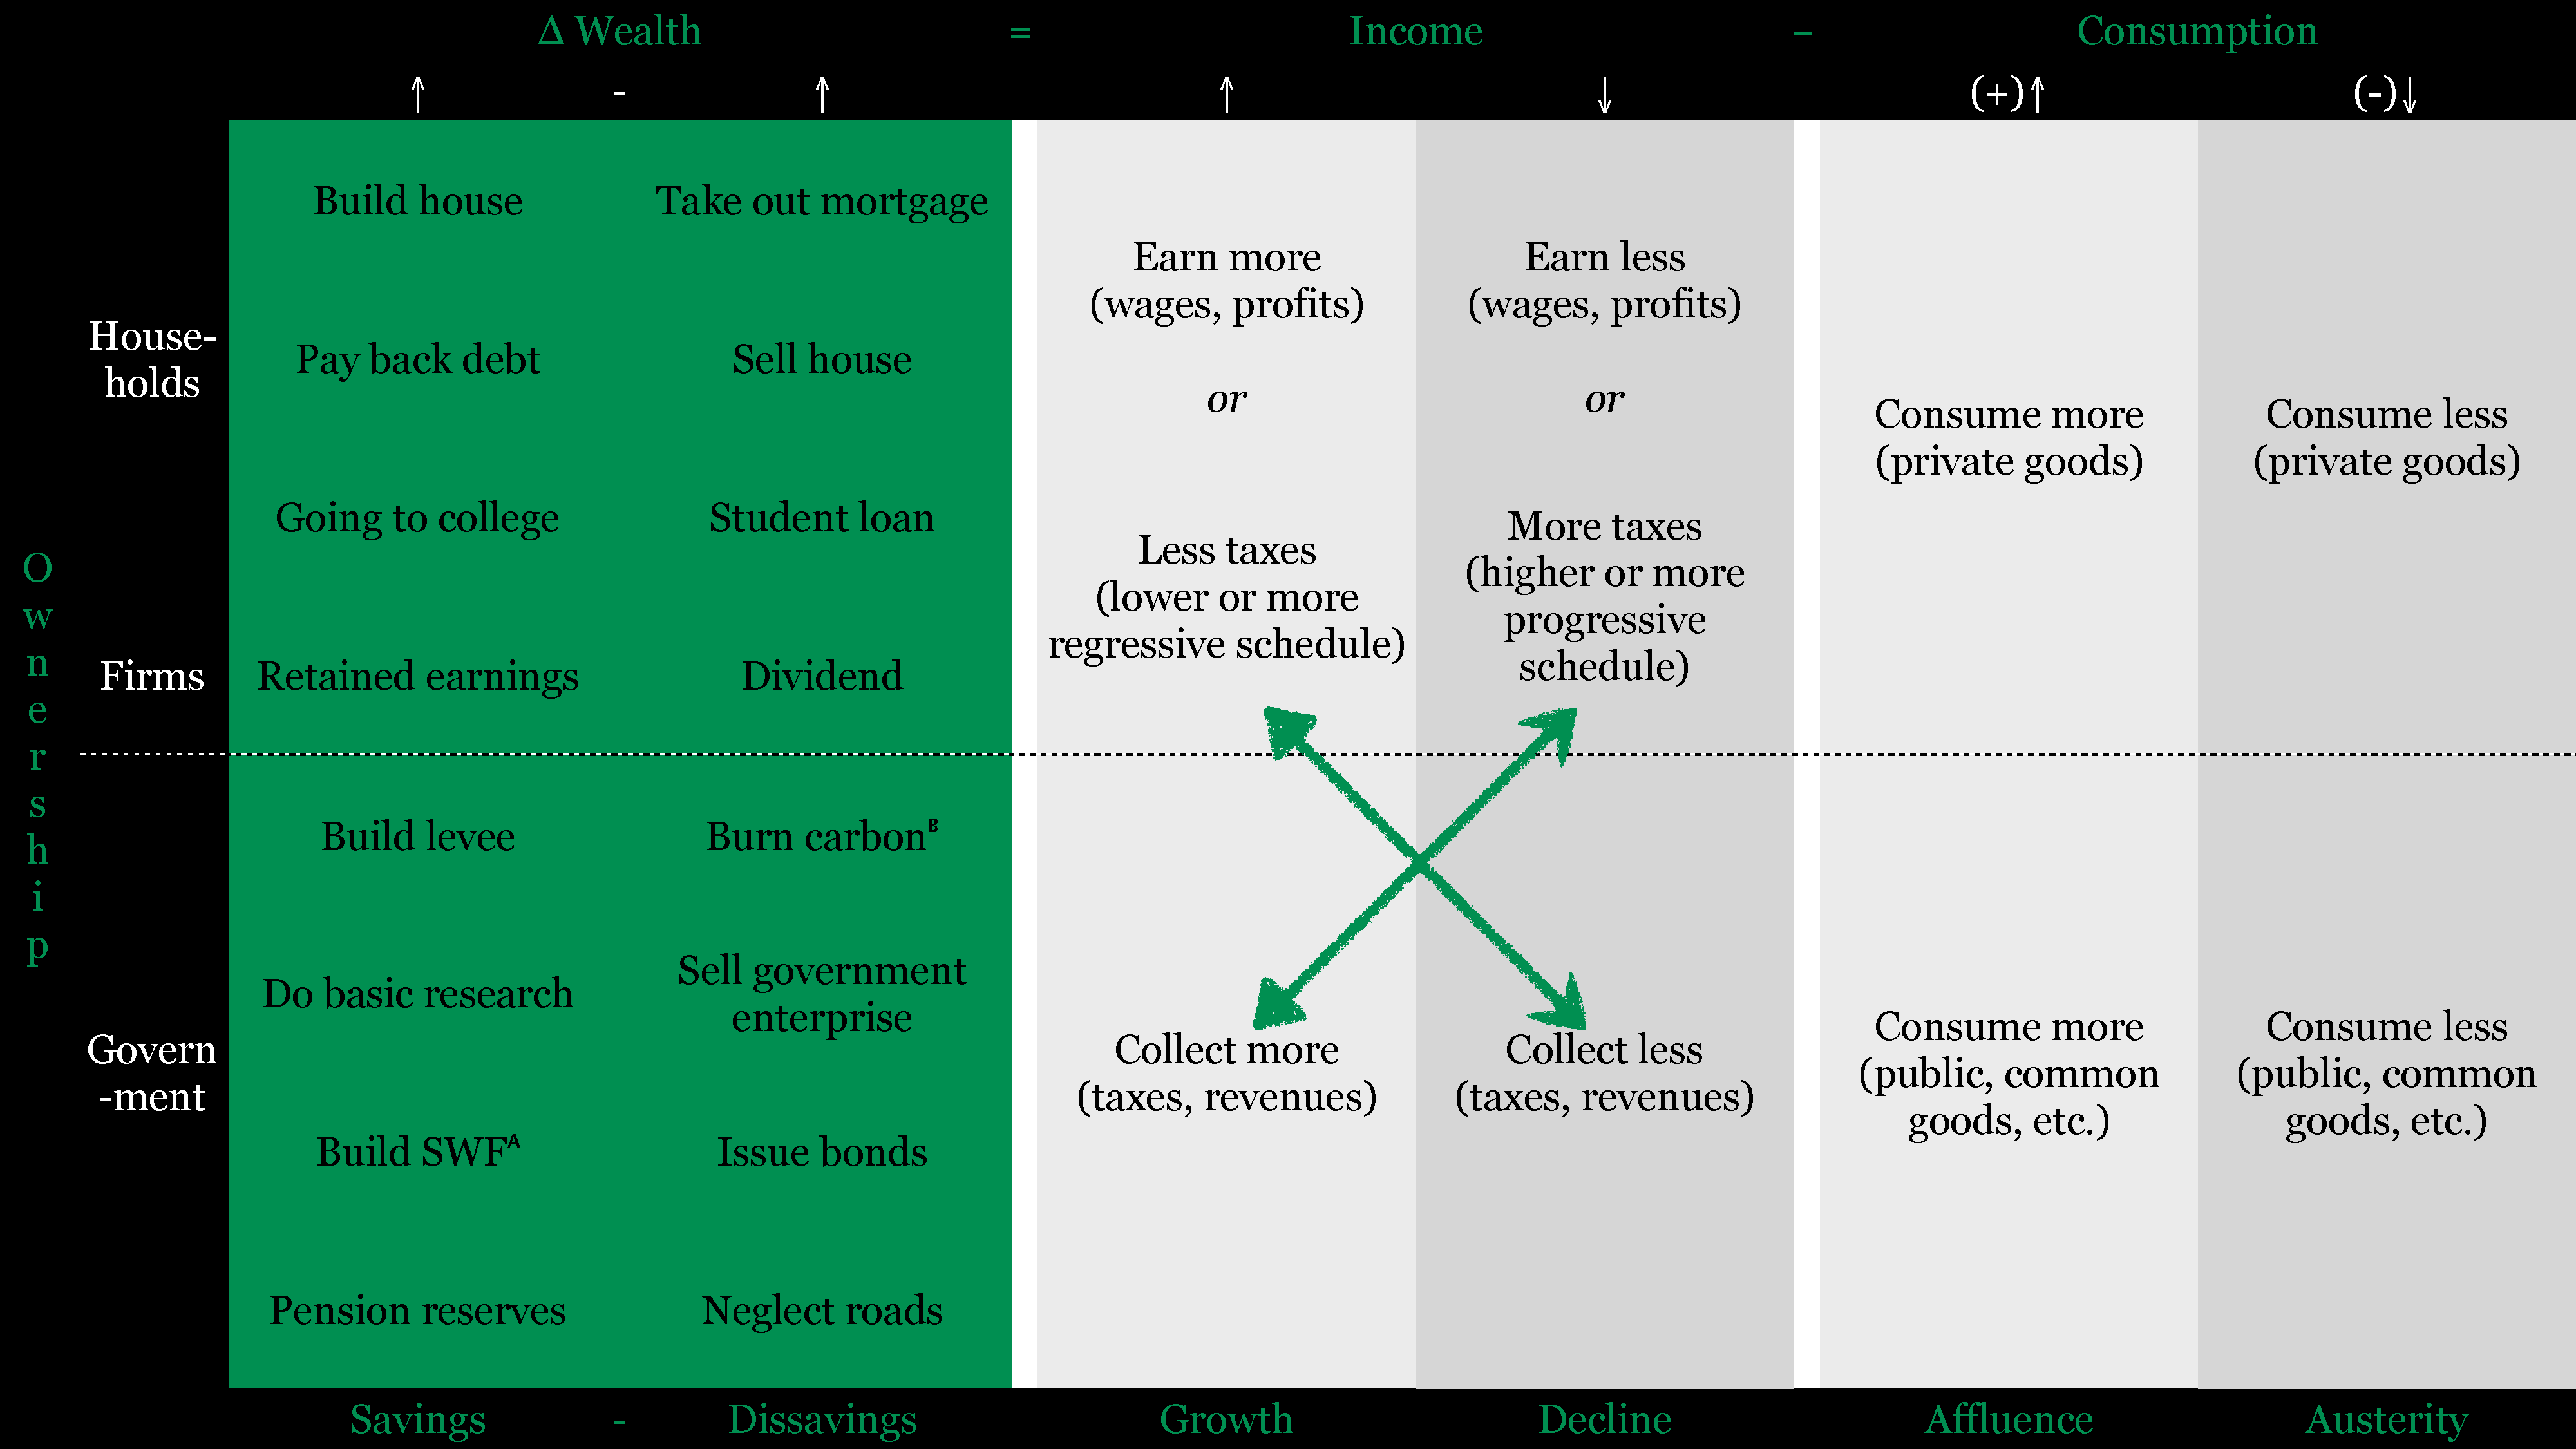
\includegraphics[width=1\linewidth]{./img/haig-simons-individual-collective}  
	\caption{Individual and Collective Haig-Simons Identity of Income}
	\label{fig:haig-simons-individual-collective} %again, no green on black please.
\end{figure}

The logic of the Haig-Simons identity, and figure \ref{fig:haig-simons-individual-collective} is easy: you can only have your cake \emph{or} eat it. Any change in consumption must be matched by a change in income or net worth --- and vice versa. 

For instance, a household can afford to build a house either by taking out a mortgage, earning more, or consuming less. 

The identity can be balanced \emph{across} households, firms and government, too. These transfers occur through different financial products and fiscal institutions. For instance, a household can also afford to build a house if it pays fewer taxes and government accepts less revenue. Government looses the amount in income that households earn\footnote{
	Strictly speaking, this would be the case only for a perfect tax with a zero \gls{DWL}.}. 

A comprehensive Haig-Simons identity also includes depreciation (e.g. neglected roads) and depleted natural resources (e.g. fossil carbohydrates) as real dissavings. For instance, an economy can consume more than it earns for some time by burning oil\footnote{
	Arguably, the past two centuries of growth in the West are to some extent due to the exploitation of fossil fuels.}. %add source to footnote.
Conversely, a comprehensive Haig-Simons identity also includes real savings such as a newly developed technology or public infrastructure, even when these are not (yet) market priced\footnote{
	Preparing a Haig-Simons account on illiquid, public or intangible assets will be difficult. As far as possible, accounting should rely on market prices, but will also have to rely on  some planned \gls{CBA}.}. 
For instance, an economy can consume less today at equal income and channel the surplus into basic research, \gls{RnD} or send more people to (costly) college.

The Haig-Simons identity of income is a truism similar to the law of conservation of matter. Surprisingly, it is often ignored or misconstrued, even in \hyperref[sec:Literature]{social-scientific literature} (p. \pageref{sec:Literature}). %refer instead here to bastard keynesianism.

I offer two notes to further clarify:
\begin{enumerate}
	\item \emph{Saving $=$ Investment.} In the long run, when industry has adapted and monetary effects have neutralized, all savings are invested. Saving does \emph{not} depress aggregate demand and choke the economy.
	
	True Keynesian shortfalls in aggregate demand result from people hording \emph{cash} or equivalents, and not because of an increase in investment. In deflationary spirals, anticipating lower prices, people cut \emph{both} consumption \emph{and} investment: the contracted money supply freezes up \emph{all} economic activity. 
	
	This popular conflation of monetary dynamics with savings rates may be one of the most formidable obstacles to enlightened, democratic choice of economic policies and tax in particular\footnote{
		In my ongoing dissertation at \gls{BIGSSS} on the pluralist and deliberative politics of taxation, I call this misunderstanding \emph{Bastard Keynesianism}, gone badly awry. I hypothesize that because people do not properly understand the Haig-Simons identity (and the economic cycle), they will erroneously assume that any tax on consumption will hurt the economy. In truth, as I argue here, an economy can take on any tradeoff between present and future consumption, if only it is phased in slowly enough.
		
		This confusion, I argue, diverts people away from optimal and fair taxation and effectively curtails the democratic sovereign in pluralism.}.
	
	Instead, saving \emph{changes}, but need not depress, aggregate demand; more capital goods and fewer consumer goods are in demand. If given enough time, the economy can transform from ``S-classes to school buildings'' without write-downs on unamortized capital investment. Well-regulated, competitive financial intermediaries will always channel saving into investment. 
	
	An investment is a valuable transformation or improved understanding of our physical world. It requires labor. Be it a \gls{SWF} or a savings account, a blast furnace or a green tech patent --- in the final analysis, saving always means to build more things that last longer and/or that we will consume later, instead of things that last a short while and that we consume now. 
	
	Of course, any \emph{one} investment will \emph{ultimately} be consumed or depreciate away. And we \emph{can} save too much, when capital goods depreciate faster and have such decreased marginal returns that they outstrip our current utility from the same resources (This follows from \cite{Solow1956} theory of growth, p. \pageref{sec:time}).
	
	But while that means we should not save endless amounts at any point in time, it does not mean that at some point in time, we should save no more. There is no economic reason why we could not roll over (limited) savings to our children in perpetuity.

%There is some linke between aggregate demand and inequality, but I forgot which one.

	\item \phantomsection \label{it:creditsdebitswash} \emph{Dissaving $\neq$ Debt $=$ Deposits $\neq$ Saving.} Dissavings are not the same as debt. Dissaving is a decrease in net worth of households, firms and economies: we diminish some durable thing in its value. Conversely, saving is an increase in net worth: we add value to some durable thing. 

%Deposits is the wrong term, it's savings and when they don't equal investments (that is a Keynesian crisis of low demand.

	In contrast, going into debt does not affect net worth of households, firms or government: we temporarily gain access to an \emph{already existing} valuable thing (construction man-hours), potentially transform it into something else (a house) and return the valuable thing later (with interest). Conversely, putting in a deposit (or other credit) also does not affect net worth: we temporarily grant access to an \emph{already existing} valuable thing to others, for an interest.

	\begin{table}[htbp]
		\caption{Debt and Credit in the Closed Economy}
		\label{tab:DebtCredit}
		\small
		\begin{center}
		\renewcommand{\arraystretch}{1.5}
		\begin{tabular}{ccc}
			\toprule
			\emph{Households} & \emph{Government}&\\
			\midrule
			$Income - Spending<0$ & $Revenue - Spending<0$&\emph{$\sum$}\\
			private debt & public debt &$=$\\
			(e.g. credit card, mortgage) & (e.g. government bonds) &\emph{All Debt} \\[20pt] 
			$Income-Spending>0$ & $Revenue - Spending>0$ &\emph{$\sum=$}\\
			private credit & public credit &$=$\\
			(e.g. deposits, bonds) & (e.g. reserves, sovereign wealth) & \emph{All Credit}\\
			\midrule
			& & $\sum=0$ \\
			\bottomrule
		\end{tabular} %double check this table, especially terminology, also consider deposits.
		\end{center}
	\end{table}

	Trivially, public and private debt will always equal public and private credits in the closed economy as summarized in table \ref{tab:DebtCredit}. By definition, every debtor needs a creditor. 
	
	Debt and credit define the short-term control of and long-term claims to valuable things and may have distributive consequences, but they do not affect net worth. Net saving, by definition, does\footnote{
		This distinction seems straightforward. Yet, similar to bastard Keynesianism, much of public debate of finance and economicsis is marred by great confusion about these basic terms. \citealt{McCaffery2005} explains how an inconsistent treatment of debt and capital gains opens up income taxation to ``tax evasion 101''.}.%make this into another big misunderstanding for my diss?
\end{enumerate}

\subsection[Smoke and Mirrors]{Smoke and Mirrors} \label{sec:smokenmirrors}

\begin{quote}
	\emph{``If it's too good to be true, it's too good to be true.''\\}
	--- The author's landlady, trained nurse, single mother of three and foreclosed homeowner in Irvine, California 2007.
\end{quote}

A mixed economy can seemingly overcome its physical limitations and the \hyperref[sec:tradeoffs]{tradeoffs} (p. \pageref{sec:tradeoffs}) between different ends using a set of smoke and mirrors. 

I briefly explain how three such practices allow us to live beyond our means in the short term:

\begin{enumerate}
	\item \phantomsection \label{it:creditbubbles} \emph{Credit Bubbles.} Within the closed economy, \hyperref[it:creditsdebitswash]{debts and credits are always ``a wash''} (p. \pageref{it:creditsdebitswash}). Still, excessive debt and credit can serve to hide or defer economic trouble ahead. 

	In efficient financial markets, credit is extended to households, firms and governments at an interest rate that fully reflects the risk of default. To assess credit risk, creditors make (and update) predictions about the future solvency (and liquidity) of debtors. 

	In the real world, these guesses are sometimes overly optimistic given the available information and credit is extended at too low an interest rate to too many people and organizations\footnote{
		Credit and concomitant asset bubbles can arise for several reasons and according to competing theories, including beauty-contest-type \citep{Keynes1936}, herding \citep{Banerjee-1992-aa} and excessive monetary expansion \citep{Stiglitz2010}. An authoritative history of financial crises is \cite{KindlebergerAliber-2005-aa}.}. 
	As long as these risks are not reappraised or do not materialize, an economy can seemingly live beyond its material means. Eventually, of course, credit bubbles will burst and debtors will partly (have to) renege on their promises to repay interest and principal. Now, the economy as a whole has to pay for the fat years.

	Credit bubbles are thus always an intertemporal redistribution of wealth from the future to the presence\footnote{
		Conversely, credit crunches, in part, redistribute wealth from presence to the future. By keeping the economy below its potential aggregate supply, credit crunches also waste capacity}. 
	When they burst, credit bubbles also jumble ownership rights as defaults spread \citep{Stiglitz2010}\footnote{
		Conventionally, as \citeauthor{Stiglitz2010} points out, a default wipes out shareholders (equity finance) and makes creditors (debt finance) into the new shareholders. In the 2007ff financial crises, as elsewhen, economic and political power often intervened to distribute the pain of default differently \citep{Stiglitz2010}.}. 
	Depending on this resulting, quintessential political-economic struggle between debtors and creditors, the brunt of the bursting bubble is allocated between different households, firms and government \citep{Coggan2011}\footnote{
		\citealt{Coggan2011} recently told the history of all hitherto existing society as the struggle between debtors and creditors, to paraphrase \cite{MarxEngels-1848-aa}. According to both \citeauthor{Coggan2011} and \cite{Stiglitz2010}, household debtors and governments assumed much of the burden during the 2007ff financial crises, causing, in part, the pursuant sovereign debt crises.}. 
	Similar to inflation and asset bubbles, bursting credit bubbles also redistribute somewhat arbitrarily based on financial product and timing: people who own equity or leave overheated credit markets early enough, win. The suckers and laggards loose.

	\item \phantomsection \label{it:assetbubbles} \emph{Asset Bubbles.} Concomitant to credit bubbles, bubbles can arise in certain classes of overvalued assets, often including real estate (2007ff), stock (2000f) but also art, oldtimers or essentially useless gold. Assets are overvalued, when their capital gains are more than what returns can reasonably be expected, given all available information. %might add piece: housing wealth isn't real wealth

	As long as prices do not revert to intrinsic value, people and the economy as a whole can live off the virtual capital gains and beyond its material means. %explain further: they're living of someone else's surplus production, that they have promised to return. 

	Asset bubbles, too, redistribute wealth from the future to the presence. In addition, as pyramid schemes, they redistribute between early investors and later, ``greater fools'' (see \citealt{Stiglitz2010} for a good discussion of the 2007ff crises).

	\item \phantomsection \label{it:inflationarypressure} \emph{Inflationary Pressure.} Excessive monetary expansion, aside from fueling credit and asset bubbles can also cause demand-pull inflation. The onset of inflation and its costs, however, need not be instantaneous. As upcoming wage-price spirals and increasing inflationary expectations silently add to built-in inflation \citep{Gordon1988}, an economy may enjoy temporarily  heightened output\footnote{
		Traditionally described as an (inward) move along the \cite{Phillips1958} curve.}. 
	As the price level eventually creeps up\footnote{
		An upward shift of the \cite{Phillips1958} curve.}, 
	the economy pays the costs of inflation through depressed growth.

	Grandfathered inflation also redistributes from the future to the presence, and arbitrarily redistributes between cash-denominated and other ownership claims, between debtors and creditors\footnote{
		In addition, the costs of later disinflation may be large. Prescriptions for disinflation and expected costs differ.}.%add literature quotes. 
\end{enumerate}

\paragraph[Too Good To Be True]{Too Good to be True.}
In summary, an economy cannot produce and consume above its long-run growth path of outward shifting aggregate supply. 

Trivially, the wealth of an economy is determined by its natural resources, technology, human and physical capital --- all \emph{tangible things}. When these capacities are fully utilized (as they are \emph{not} in a cyclical downturn or debt-deflation crisis), no financial or monetary charlatanism can take us beyond them in the short term. Any short-term gain that a bubble or excessive monetary expansion will bring only defers the day of this reckoning.

\subsection{Real Dissavings} \label{sec:realdissavings}

\begin{quote}
	\emph{``When the last tree is cut, the last river poisoned, and the last fish dead, we will discover that we can't eat money.''\\}
	--- Greenpeace
\end{quote}

Our economies substantially dissave in ways that are not reflected in conventional macroeconomic data. These \emph{real} dissavings, or ``off-budget fiscal activities'' (\citealt{Bonker2006}: 49) include population aging\footnote{
	The second demographic transition (\citealt{Davis1945}, restated by \citealt{Caldwell-1976-aa}) delivered low, often below-replacement level \gls{TFR}.}, 
depleted natural resources (land, oil, water), exhausted common goods (global warming\footnote{
	The greatest, widest-ranging market failure in the history of mankind, according to \cite{Stern-2006-aa}.}) 
or failed public goods (immunization?), to name just a few. 

These processes all unambiguously degrade something of economic value, and should be recorded as consumption in our aggregate Haig-Simons accounts (as I have suggested in figure \ref{fig:haig-simons-individual-collective}, p. \pageref{fig:haig-simons-individual-collective}). %wuppental institute has some accounting data on this. %is this the right fig label?

\subsection[Why it Matters]{Why it Matters: The Welfare State as Mixed Economy} \label{sec:whymixedeconomymatters}

\begin{quote}
	\emph{``Yes we can: to justice and equality.\\ Yes we can: to opportunity and prosperity.''\\}
	--- Barack H. Obama, Obama For America 2008
\end{quote} %better quote, anyone?

At this point, a reader may ask: why would all, or even any of this, matter to the welfare state?

Materially possible and normatively desirable welfare states are, and must be thought of as, well-designed mixed economies, for at least three reasons:

\begin{enumerate}
	\item \emph{Engaging Complexity.} In a welfare state, \hyperref[sec:interface]{exchange and command modes of production and distribution, inevitably, complexly interact and easily produce unintended consequences} (p. \pageref{sec:interface}). For example, a \hyperref[sec:princecontrols]{minimum wage may cause structural unemployment} (p. \pageref{sec:pricecontrols}) and the \hyperref[sec:well-determinedincidence]{\emph{nominal} incidence of a tax will be entirely inconsequential} (p. \pageref{sec:well-determinedincidence}). 
	
	To eradicate today, as Lord Beveridge promised 150 years ago, the five `Giant Evils' of want, disease, ignorance, squalor and idleness, you have to anticipate this interplay of market and government and choose accordingly. The mixed economy provides us with a toolset to analyze the complexity of welfare states, including the dynamics presented here. For example, the mixed economy suggests we should always check the \gls{DWL} (p. \pageref{sec:minimalDWL}) and \hyperref[sec:well-determinedincidence]{incidence} (p. \pageref{sec:well-determinedincidence}) of any redistribution, a welfare state may undertake.
	
	To answer the first-order question of welfare state design, as I have here tried to do, we need the abstractions of the mixed economy to know what is \emph{materially possible} in a scarce world, filled with (at least some) homines oeconomici. For example, price controls may not be possible (without grave losses), but a well-designed, personal, almost arbitrarily progressive taxation \emph{is} indeed possible in a closed economy.	
	
	\item \emph{Denaturalizing Market Allocations.} When we consider welfare state programs in isolation from the markets which they supplant, we easily end up naturalizing whatever markets have allocated. In fact, any given market exchange which a welfare state may seek to correct, is already and always \emph{contingent} on the institutions, dynamics and distributions under which it occured. 
	
	For example, rather than ``fighting poverty'' --- as if that were an objective reality --- welfare states must consider overall allocative dynamics (such as \hyperref[sec:winner-take-all]{winner-take-all}, p. \pageref{sec:winner-take-all}) and distributions (such as \hyperref[sec:monopsonyemployers]{monopsony employers}, p. \pageref{sec:monopsonyemployers}), and counteract them, as is seen fair. Markets do not make some people below an arbitrarily defined threshold ``poor'', and leave others ok or even untouched. Instead, markets allocate incomes across the \emph{entire} spectrum contingent on a host of institutions, dynamics and initial distributions. If government pursues a particular minimum standard of living for everyone, it might not only transfer income to those who fall below it, but may need to counteract those dynamics under which people slipped below the minimum standard in the first place. 
	
	Market allocations, in short, are --- and should be --- no less subject to enlightened, collective human choice than remedial welfare state programs: ``Increasing dependency is no law of nature but the result of socio-economic changes, which in turn react to human intervention'' (\citealt{Esping-Andersen2002}: x).
	
	\item \emph{Caring about Outcomes.} \citeauthor{Haggard2009} (\citeyear[236]{Haggard2009}) remind us about
		\begin{quote}
			``(\ldots) the importance of pushing the research on the [Eastern European] welfare state down the causal chain towards its social consequences. (\ldots) [A]ny meaningful strategy of comparison of the welfare state must ultimately engage its consequences for a variety of outcomes, from poverty and inequality, to physical quality of life measures, to economic outcomes such as the efficiency of labour markets, competitiveness and even economic growth. In the first instance, we are interested in the welfare state because we are interested in human welfare.''
		\end{quote}
	
	The abstractions of the mixed economy I have summarized here synthesize a lot of what we need to know about the material, and therefore social consequences of a capitalist welfare state. 

	When we care about social consequences, the mixed economy suggests a great deal more to consider than just nominal welfare programs. For example, welfare states should not only provide social insurance, but also redress failing \hyperref[sec:publicgood]{public goods} (p. \pageref{sec:publicgood}) and \hyperref[sec:long-terminconsistency]{make us save enough for our children} (p. \pageref{sec:long-terminconsistency}). 
	
	When we care about social consequences, the mixed economy also implies that not all welfare programs are created equal. For example, welfare states interventions should \hyperref[sec:minimalDWL]{distort market prices as little as possible} (p. \pageref{sec:minimalDWL}) and use \hyperref[sec:pricestability]{monetary expansion only sparingly, for short-term stimulus} (p. \pageref{sec:pricestability}).
	
	When we care about social consequences, the mixed economy suggests that  governments and markets are better at different things, and it ties welfare state interventions to specific justifications. For example, welfare states should nationalize or regulate utility markets if and to the extent that they are \hyperref[sec:naturalmonopoly]{natural monopolies} (p. \pageref{sec:naturalmonopoly}), but there is no reason to (as Germany presently does) redistribute within \hyperref[sec:stateinsurance]{social health insurance} (p. \pageref{sec:stateinsurance}), who was supposed to only save the risk pool from \hyperref[sec:adverseselection]{adverse selection} (p. \pageref{sec:adverseselection}). Caring about social consequences also means to leave markets alone, if they will likely serve material human need best.
	
	When we care about social consequences, the mixed economy reveals that efficiency and equity are not always opposed, but often go hand in hand. 
	\begin{enumerate}
		\item \emph{Inefficient is Inequitable.} \citeauthor{Titmuss1974} urged welfare states not to exclusively concentrate on poverty relief because such ``residual services (\ldots) often become poor services for poor people'' (\citeyear{Titmuss1974}: 134). This intuition is supported by the abstractions of the mixed economy: as the rich are forced or allowed to take the inefficient --- but for them, affordable --- exit route from government provision, a retrenched welfare state will offer only inferior provision, or none at all, to those too poor to exit. 
		
		This problem is particularly acute in health or disability insurance: as the rich and healthy exit the risk pool, coverage becomes ever more expensive, driving even more people out until it \hyperref[sec:adverseselection]{fails} (p. \pageref{sec:adverseselection}). 
		
		Similar distributive effects occur in a wider class of market failures, too. For example, a failed \hyperref[sec:commongood]{commons} (p. \pageref{sec:commongood}) of global climate or local public safety will not only be wastefully inefficient, but it will also hit hardest the poorest regions and people, who can least afford substitutes, such as building a levee or hiring private protection. 
		
		\item \emph{Inequitable is Inefficient.} On the other hand, the abstractions of the mixed economy also imply that sometimes, slicing the pie unequally, will also make it smaller: ``(\ldots) there is a very good argument that equality of opportunities and life chances is becoming sine qua non for efficiency as well'' (\citealt{Esping-Andersen2002}: ix).
		
		For example, people may not be able to align the \hyperref[sec:principal-agentproblem]{interests of principals and agents} when collateral is not widely available (p. \pageref{sec:principal-agentproblem}), and overly taxing low and middle (labor) incomes may contribute to \hyperref[sec:minimalDWL]{structural unemployment} (p. \pageref{sec:minimalDWL}).
	\end{enumerate}
	
	To answer the first-order question of welfare state design, as I have here tried to do, we need the abstractions of the mixed economy to know what is \emph{normatively desirable} in a scarce world, filled with (at least some) homines oeconomici.	
\end{enumerate}

\paragraph[Higher Equilibria]{Higher Equilibria.} The first-order conflict about the best, possible welfare state is about the tradeoffs, contradictions and uncertainties of the mixed economy explained in the above. My aim here was not to resolve that conflict: we may not know for sure, let alone agree on what \emph{the best} welfare state looks like (even though I offered some well-informed hunches). A mixed economy can --- in principle and for my purposes here --- make \emph{arbitrary} tradeoffs between equity and efficiency, presence and future, or any of the other dimensions of human material need. 

But given \emph{any} preference set for these (sometimes!) competing goals, there are still more and less efficient institutional configurations for the mixed economy. More efficient, in this broadest sense, means that these configurations achieve more on \emph{all} goals. These preferable mixed economies will still trade off preferred goals for less preferred goals, but the tradeoff will be less harsh. For example, a \gls{NIT} may achieve the same, if not more equity than a minimum wage, but at much lower cost in growth, or unemployment. Of course, you still have to break eggs for the proverbial omelette, just fewer of them.

The competing goals of human material need, in other words, are not always in a pure and immutable zero-sum relation, where, for example, one increment more in equity means one less in efficiency, one more in present consumption one less in future consumption. Depending on the institutional design, these conversion rates will differ: sometimes, for example, one increment in equity will cost only a half-increment in efficiency. Alternative mixed economies, more often than not, are a positive or --- equivalently --- negative sum proposition. 

Just entering the preferences between purposely competing goals does \emph{not} yield a single configured mixed economy, but many different blends of command and exchange production and distribution. Again, we may not know or agree what the globally optimal configuration is, given our preferences, but checking \hyperref[sec:means]{means} and \hyperref[sec:ends]{ends} of a mixed economy, we \emph{can} know better from worse configurations, or local optima.

A better welfare state is that mixed economy which elegantly combines \hyperref[sec:command]{command} and \hyperref[sec:exchange]{exchange} components to \hyperref[sec:production]{produce efficiently}, \hyperref[sec:risk]{pool risks}, \hyperref[sec:distribution]{distribute equitably}, \hyperref[sec:time]{consistent over time} and \hyperref[sec:space]{convergent over space}. That is, a welfare state that offers one of the higher possible tradeoffs of growth, individual security, equality, saving and convergence. It does so without effectively borrowing from the future through \hyperref[sec:smokenmirrors]{smoke and mirrors}, or hidden, but \hyperref[sec:realdissavings]{real dissavings}. 

%Do I need the next section in the thesis? It might not fit.

This view of the welfare state differs markedly from other perspectives:
\begin{description}
	\item[Full Employment or Growth.] A popular variant on the purposive tradeoff between equity and efficiency, is that between the policy goals of full employment or growth, sometimes supported by ``demand-'' or ``supply-side'' economics. %make a footnote about this.
	%might need a bigger section about this, maybe with bastard keynesianism.
	\citeauthor{Offe2003} \citeyearpar[453]{Offe2003} finds a similar controversy about how to best keep up the full employment ``roof'' over the metaphorical Keynesian welfare state house, protecting the lower floors: market liberals (or supply-siders) want to deregulate so that \emph{growth leads to more employment} and social democrats (and, sometimes, demand-siders) want to sustain welfare state protection so that \emph{more employment stimulates growth}. 
	
	These contenders both once had a (somewhat overstated) point, but as market failures grew and monetary policy improved, they are now both increasingly wrong. 
	
	Market liberals are wrong because not all deregulation, or any amount of it, will stimulate growth, and conversely, not all redistribution or other intervention will depress growth. The abstractions of the mixed economy suggest that sometimes, command production is more \hyperref[sec:marketfailures]{efficient} (p. \pageref{sec:marketfailures}).
	
	Social democrats, or more accurately, demand-siders are wrong because, of course, in the long run, \emph{only} supply determines prosperity, and the depressed aggregate demand they \emph{always} seem to suspect is clearly defined as a monetary phenomenon and unlikely to persist for very long. If it occurs, monetary expansion and fiscal stimulus should smooth it out, but that does not make for a roof. Social democrats are also wrong to believe that all redistribution and regulation is cost-free: there \emph{are} \glspl{DWL}. 
	
	The indicators of \emph{activity} that both market liberals and social democrats usually obsess about --- \gls{GDP} and full employment respectively --- are both emphatically not related to greater \hyperref[sec:tradeoffs]{Haig-Simons incomes} (p. \pageref{sec:tradeoffs}). And so, they both sometimes fall for \hyperref[sec:smokenmirrors]{smoke and mirrors} (p. \pageref{sec:smokenmirrors}) and ignore \hyperref[sec:realdissavings]{real dissavings} (p. \pageref{sec:realdissavings}). %reference earlier footnote.
	
	So how can we rescue full employment? By \emph{not} fighting this last war, for at least two reasons.
	
	\begin{enumerate}
		\item Pushing macroeconomic policy to full employment risks overheating the economy and building up inflationary pressure.
		\item More fundamentally, full employment no longer is (if it ever was) a necessary, let alone sufficient factor for anything we might consider socially desirable outcomes for a welfare state. Full employment in itself cannot, as the house metaphor suggests, provide any shelter for depleted \hyperref[sec:commongood]{commons}, lemon-market \hyperref[sec:adverseselection]{risk pools}, let alone address intertemporal failures or bubbles, to name just a few. More dearly to social democrats, full employment will also be increasingly unable to --- as the proponents of power resources had hoped --- level the playing field between capital and labor, simply because some of the major inequities no longer are between capital and labor, but also \emph{within} labor incomes as \hyperref[sec:winner-take-all]{winners-take-all} (p. \pageref{sec:winner-take-all}). Even if the ``reserve army of the unemployed'' is fully activated, the resulting upward pressures on low (or all) wages will be no match for the governing dynamics of inequality enveloping the postindustrial economy (such as Baumol's cost disease). 	
	\end{enumerate}
	
	Full employment, and (properly defined) growth are still desirable --- because they are an efficient \emph{outcome} --- but neither serves as a powerful \emph{instrument} to reduce poverty or economic insecurity: ``Promoting labour market participation is no substitute for income redistribution and the fight against poverty: more work does not necessarily mean less poverty'' (\citealt{Esping-Andersen2002}: ix). \citeauthor{Offe2003}'s metaphorical house of the Keynesian welfare state, in other words, does not need a few new shingles, but an altogether new roof. 
	
	That new roof is the ability of the mixed economy to redistribute, efficiently and progressively as the democratic sovereign wishes. With that ability, welfare states can subsidize any (however small) minimal labor market income to any desired minimum standard of living (for example, through a \gls{NIT}), and can provide any level of social protection desired without counterproductively burdening low incomes (for example, by paying social insurance out of general tax revenue). Progressive redistribution could, if desired, dampen or counteract any existing income dynamic, including \hyperref[sec:winner-take-all]{winner-take-all} markets. \citeauthor{Offe2003} may be right that the welfare state did not ``have much to do with `equality of outcomes''', but that does not make it tenable or desirable today (\citeyear{Offe2003}: 450). If you are serious about even just ``security and protection of workers, not equality'' (\emph{ibid.}) you have to care about inequality and redistribution, at least a little. Without it, you will not have the resources to guarantee even such minimal, unequal outcomes for workers. I further develop this argument  in my \hyperref[sec:Pangloss]{Panglossian} critique of the literature (p. \pageref{sec:Pangloss}).
	%this might need to be consolidated with the re-entrnechement part.
	%Voltaire:      The rich require an abundant supply of poor.

	\item[Decommodification] still serves well to distinguish different welfare states \citep{Esping-Andersen-1990-aa}, but it, too, is no strategy for a possible and desirable mixed economy.  Of course, welfare states may still ``decommodify'' (or \emph{subsidize}) health care, education and replace (or \emph{insure}) the incomes of the sick, disabled, old and unemployed, but such programs may be better described in the language of the mixed economy: as \emph{specific} market interventions and redistribution. 
	
	The difference is not merely semantic, but at least three substantial misunderstandings easily follow from this choice of terminology:
	\begin{enumerate}
		\item Decommodification suggests --- misleadingly --- that welfare states \emph{could} take some aspects of life, and some people \emph{off} the market. But, because command and exchange modes of production and distribution always interact, that cannot be done. 
		
		For example, decommodification of disability income is easily misconstrued to mean that disability would no longer be affected by the market, and that markets would no longer be affected by disability. That is not so. When welfare states support the disabled, they not only exempt them --- as intended --- from earning a market income, but they may also make it cheaper, and therefore more likely for labor markets to \emph{produce}, say, burn-out, depression or back pain. 
		
		Thinking in the abstractions of the mixed economy helps us to avoid such pitfalls. In this case, we know that \emph{insurance} of risks is prone to moral hazard, and that (Pigouvian) co-payments can save the commons of a prudent risk-pool. We can, if desired, slap a Pigouvian tax on risky or strenuous employment and activities, to make sure it is more costly, and is avoided.
		
		\item Decommodification easily morphs from description to prescription, as for example, when income replacement becomes a measure for welfare state re- or entrenchment. %add source
		Caring about outcomes, there is nothing inherently desirable or essential about decommodification, for four reasons:
			\begin{enumerate}
				\item To decommodify someone out of the market also means to exit someone out of the central institution, that aside from providing the substituted material sustenance, mediates much human cooperation, generates self-worth to many and allows people to shape the world around them, however marginally. Instead, we should ``enable all citizens to participate in the mainstream of social and economic life'' (\citealt{Esping-Andersen2002}: ix).

				\item Complete decommodification is a last resort response to hardship. Mixed economies have several alternative, and less intrusive, approaches to, for example long-term unemployment. Instead of generous, universal and unconditional --- and therefore decommodifying --- benefits, a mixed economy may subsidize low market wages with a continuous and regressive \gls{NIT}. 
				
				The availability of a \emph{specific} tool, may not much matter to the desirability of a welfare regimes: social outcomes do.

				\item Decommodification, conceptually, if not always in reality, is ignorant of potential welfare losses, as some person is provided, or some activity done under command instead of exchange --- without a respective, justifying market dysfunction. Thinking instead, in the abstractions of the mixed economy, always ties a market intervention to a particular market failure or broader dysfunction, and considers the potential welfare losses.
			\end{enumerate} 
			
		\item Decommodification is both radical as a prescribed tool (exit the market) \emph{and} strictly limited in its reach (only a set of included people or activities). To be sure, sometimes a complete move to (entitled) command provision and distribution may be necessary or desirable. Likewise, a democratic sovereign may choose to only care \emph{a lot} about some market outcomes --- and decommodify them ---, and not care about others \emph{at all}. But there is no reason that all welfare states should do so, let alone that we carve this specific vision of a social compact into our conceptual toolbox.
	\end{enumerate}
\end{description} 

\paragraph{It follows:} for a better welfare state to strike any such optimal balance, even given arbitrary preferences, it needs an intact set of \hyperref[sec:regulatory]{regulatory} (p. \pageref{sec:regulatory}), \hyperref[sec:fiscal] {fiscal} (p. \pageref{sec:fiscal}) and \hyperref[sec:monetary]{monetary} (p. \pageref{sec:monetary}) \hyperref[sec:means]{means} of a mixed economy. %this sentence could be better. u

Of these, tax is the elephant in the room: it is by far the most versatile, precise and powerful tool of command production and distribution in the mixed economy.

None of this is a merely abstract or academic concern. Much lies this balance of command and exchange: everything we materially value, and with that, a great deal of the life chances of us all depends on an intact mixed economy.

This is also not a revolutionary project. It does not ask for a new man, but it accepts, and timidly merely reforms \emph{homo economicus}, the civilized version of our selfish demons. It does not ask for a new institution, it carefully compromises existing ways of exchange and command. The mixed economy, by any historical standard, is not a radical proposition. 

This much, I hope, is widely agreeable.